%============================================================================
% CCM Tools Manual
%=============================================================================

\documentclass[12pt]{book}

\usepackage[latin1]{inputenc}
\usepackage{listings}


% PDF Document Info
\expandafter\ifx\csname pdfoutput\endcsname\relax
    \usepackage[draft]{hyperref}
    \usepackage{graphicx}
    \DeclareGraphicsExtensions{.eps,.fig}
\else
    \usepackage{hyperref}
    \hypersetup{
        pdfauthor={Egon Teiniker},
        pdftitle={CCM Tools Manual},
        pdfsubject={CORBA Component Model Tools},
        pdfkeywords={CCM, CORBA, components}
    }
    \pdfcompresslevel=9
    \usepackage[pdftex]{graphicx}
    \DeclareGraphicsExtensions{.pdf,.png,.gif,.jpg}
\fi


\setlength{\textwidth}{15 true cm}
\setlength{\textheight}{22 true cm}
\oddsidemargin  0.5 cm
\evensidemargin 0.5 cm
\topmargin      0 cm
\setlength{\parindent}{0cm}

\setcounter{tocdepth}{5} 


\begin{document}
%=Content====================================================================== 
	\pagenumbering{roman}
	\begin{titlepage}

\centering

\vspace*{20mm}
{\huge ccmtools.sourceforge.net }
\vspace{20 mm}

\centerline{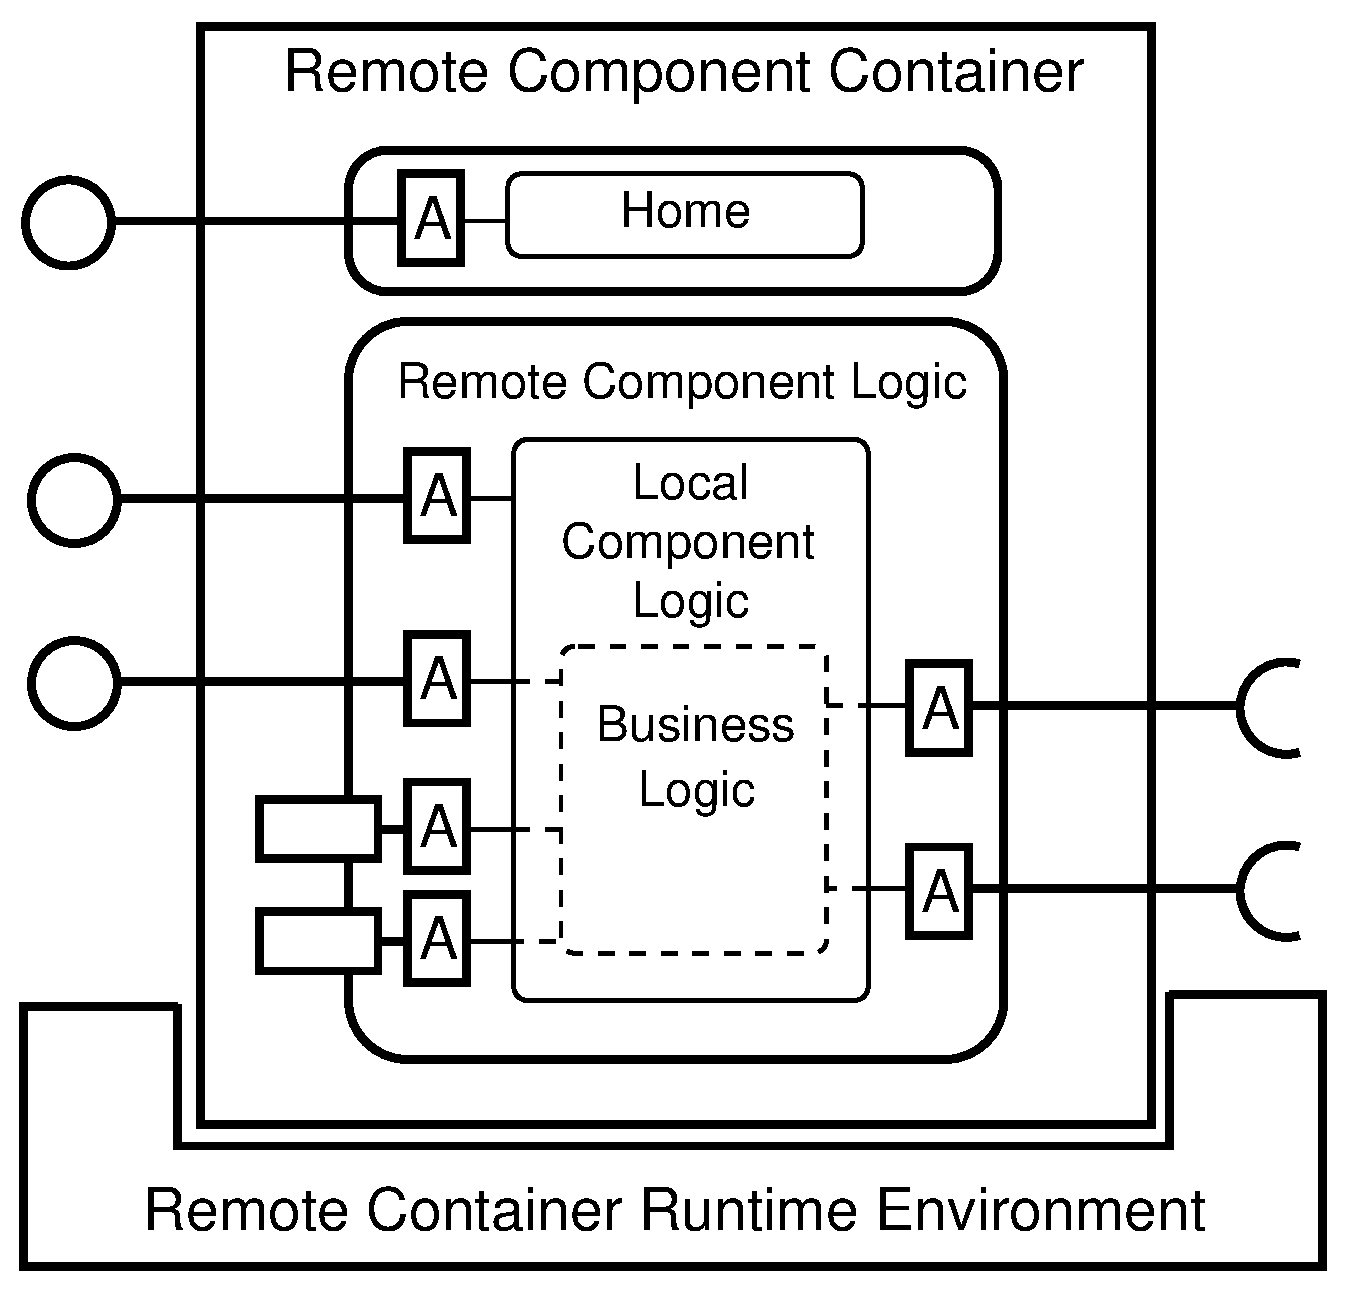
\includegraphics[width=55mm]{figures/LocalAdapterConcept.eps}}

\vspace{30mm}

{\Huge CCM Tools IDL Manual}\\ 
\vspace{5mm}
{\bf Egon Teiniker <egon.teiniker@salomon.at>}\\
\vspace{30mm}


{\Large \bf Version: 1.0.0} \\
\vspace{5mm}
$Id$
\end{titlepage}
	\tableofcontents
	\pagenumbering{arabic}

	%******************************************************************************
\chapter{Introduction}
\label{chapter:introduction}
%******************************************************************************

The CCM Tools are a set of programs and libraries used to generate, package and
deploy CORBA components. The tools implement parts of the CCM specification
\cite{CCMSpecification} with some extensions to improve the usability and
performance of the component model. The {\it CCM Tools User's Guide\/} provides
instructions for using the CCM Tools. This document, the {\it CCM Tools
Developer's Manual\/}, is aimed at developers and provides details on the inner
workings of the CCM Tools.

\begin{figure}
\centering \includegraphics[width=14cm]{ToolsOverview}
\caption{Parts of the CCM Tools package.}
\label{fig:intro-ToolsOverview}
\end{figure}

To help the component developer, the CCM Tools provide the tools shown in
Figure~\ref{fig:intro-ToolsOverview}. These tools include the following parts:

\paragraph{CCM Metamodel Library}

The CCM specification defines a metamodel for the IDL3 syntax. This metamodel is
a set of classes that are capable of representing the syntactic elements in
IDL3. We implemented a metamodel library in Java that allows creation of, and
navigation through, CCM models. Using this library we can clearly separate the
parser and the code generators, using a CCM model as the communication between
the two parts. The parser creates a model object for every part of the source
code matching an IDL grammar rule, and the generator tools read the model to
generate code. Chapter~\cite{chapter:ccm-metamodel-library} describes the CCM
Tools' construction of the CCM metamodel library.

\paragraph{IDL3 Parser}

The IDL3 Parser reads an IDL3 file, checks the syntax of the IDL source code and
creates a CCM model, using the CCM metamodel library, in memory. This CCM model
is the starting point for all code generator tools.
Chapter~\cite{chapter:idl3-parser} describes the IDL3 parser in detail.

\paragraph{Mirror Component Generators}

After building a component it is a good idea to run a set of functional tests on
it. Such testing can provide helpful component specific debugging and prevent
large, difficult to locate, system bugs later in development.

To provide a test environment for every component, the CCM Tools can create a
mirror component (a facet becomes a receptacle and vice versa) described in a
mirror IDL3 file. We use the C++ component generators with the mirror IDL3 files
to generate the code for mirror components. Then we use a C++ mirror test
generator to create a basic test executable that connects each component with
its mirror and calls the functions available for each component.

\paragraph{IDL2 Generator}

To implement CORBA components, IDL3 source code needs to be reduced to IDL2,
which can be interpreted by classic IDL compilers. The transformation from IDL3
to IDL2 also adds some operations needed for navigation between components and
their ports (equivalent operations). The CCM Tools support this transformation
using an IDL2 generator tool that creates IDL2 code based on a CCM model.

\paragraph{Component Descriptor Generator}

To describe the component for the deployment and assembling processes, the OMG
defines a {\it CORBA Component Descriptor} (CCD) file. This is an XML file
containing a short description of a component and its ports. We map the CCM
model to an XML--DOM tree that can be written as an XML file. The CCD file is
also used by the code generators to get some additional information about the
components being generated (version, vendor, etc.).

\paragraph{Local C++ Component Generator}

The CCM Tools include a generator tool that creates the local component logic
from a given CCM model. The generated code contains C++ implementations of a
component that can run in the same address space (hence called a `local
component'). This implementation includes operations for providing, using,
connecting, and disconnecting components and their facets. These generated
operations are referred to as {\bf component logic}. After generating the
component logic, the component developer needs to write the {\bf business
logic}; that is, the functional implementation of the component so that it
becomes useful in a component based software system. See
Chapter~\cite{chapter:component-generator-tools} for more information about the
component generator library.

\paragraph{Remote C++ Component Generator}

Note that the local components can only be used in a common address space and
must be implemented in the same programming language. To overcome these
limitations, the CCM Tools have a remote component generator that produces C++
code to interface the local components with CORBA. The remote component logic is
thus a superset of the local component logic.

\paragraph{UML Parser}

Optionally, the description of the component's interfaces can be contained in a
UML diagram. We need a UML parser that reads the UML--XMI file, builds a UML
model (based on the UML metamodel defined by the OMG) and transposes the model
to a standard IDL3 file. The CCM Tools can use the NSUML UML metamodel library
from NovoSoft, but the OMG has not yet defined an UML profile for the CCM. Thus
a UML tool will likely be on the back burner for some time.

\paragraph{Component Packaging Tool}

After generating and writing the component logic and the component descriptor
file, we have to package these files into a zip file called, predictably, a
component package. The component packaging tool provides these functionalities
to the component developer.

\paragraph{Component Deployment Tool}

On the target host the component package must be unzipped and the component must
be deployed in the application server. The component deployment tool provides
these functionalities to the component deployer.

\section{Assembly tools}

After creating the component logic and writing the business logic, we can use
the component from a simple client program. A big advantage of the CORBA
component model is the ability to connect components together to form larger
structures called {\bf component assemblies}.

A component assembly is a set of components (with their component descriptors)
and a {\it Component Assembly Descriptor} (CAD). Based on the CAD we can
generate an assembly object that instantiates components and connects them
together to form a component assembly.

\begin{figure}
\includegraphics[width=14cm]{AssemblyTools}
\caption{CCM component assembly tools.}
\label{fig:intro-AssemblyTools}
\end{figure}

Figure~\ref{fig:intro-AssemblyTools} provides a diagram of the assembly tools in
the CCM Tools. These tools include:

\paragraph{Assembly Descriptor Generator}

The component descriptor files are the base for the higher--level assembly
descriptor, which describes the components of the assembly and their
connections. That means that all information of the assembly descriptor comes
from the component descriptors of the related components (and some additional
data from a GUI).

\paragraph{Assembly Object Generator}

At runtime a managing object is needed that can establish an assembly instance.
The assembly object creates the component instances and connects their
receptacles and facets. All information for generating an assembly object comes
from the assembly descriptor (or its DOM model in memory). Note that this object
must eventually be able to create local or local/remote assembly instances.

\paragraph{UML Parser}

As with components, there should be a way to define component assemblies in a
UML diagram. Therefore we need a UML parser that reads the UML--XMI file and
translates the data into the DOM model used by the assembly descriptor. The OMG
has not yet defined a mapping between UML and CCM assemblies.

\paragraph{Assembly Packaging Tool}

After generating the component assembly and its descriptor file we have to
package these files into a zip file called a component assembly package. The
assembly packaging tool provides these functionalities to the assembly
developer.

\paragraph{Assembly Deployment Tool}

On the target host the component assembly package must be unzipped and the
assembly must be deployed in the application server. The assembly deployment
tool provides these functionalities to the assembly deployer.

\section{Testing}

Another important issue is {\bf testing}. We have to test our applications on
different levels during development, as listed below:

\paragraph{Class Level Testing}

Every class of the business logic that will be part of a component has to be
tested.

\paragraph{Component Level Testing}

For every component we create a counter component that looks like a mirror to
the original component. This counter component has an receptacle for every facet
of the original component and vice versa. Connecting a component with its mirror
component with a simple test client allows component developers to quickly
isolate component level errors in the business code.

\paragraph{Assembly Level Testing}

After testing each component, we have to be sure that a set of connected
components, the component assembly, also works correctly.

Of course, there must be tool support for testing on these different levels of
development to make this job more efficient.


	
	%==============================================================================
\chapter{Hello World Example}
\label{HelloWorldComponent}
%==============================================================================

As a quick tour through CCM Tools, we implement a simple Hello World 
component example. 
Each development step and developer role will be described 
in more detail in one of the next sections, here we give a general overview.

\vspace{5mm}
\noindent
{\bf Step 1:} We define a component using the 
{\it Interface Definition Language} (IDL). 
This simple component only provides a single interface containing a single
method. Don't forget to define a home for this component type.
The following IDL definitions are stored in
a file called {\tt Hello.idl}:
\begin{small}
\begin{verbatim}
module world
{ 
    interface Hello 
    { 
        string sayHello(); 
    }; 

    component Server 
    { 
        provides Hello hello;
    }; 

    home ServerHome manages Server
    {
    };
};
\end{verbatim}
\end{small}


\noindent
{\bf Step 2:} Generate a uniform IDL3 structure from the single {\tt Hello.idl}
file:
\begin{small}
\begin{verbatim}
> ccmidl -idl3 -o server/idl idl3/Hello.idl
\end{verbatim}
\end{small}

\noindent
This uniform IDL3 structure separates between interfaces (including 
parameter type and exception definitions) and components (including their
homes). Such a separation makes sense because an interface can be used by
many component definitions.
\begin{small}
\begin{verbatim}
    server/
     |-- idl
     |   |-- component
     |   |   `-- world
     |   |       |-- Server.idl
     |   |       `-- ServerHome.idl
     |   `-- interface
     |       `-- world
     |           `-- Hello.idl
\end{verbatim}
\end{small}


\noindent
{\bf Step 3:} Generate an empty component skeleton from the uniform IDL3 
structure:
\begin{small}
\begin{verbatim}
> ccmtools c++local -o server/interface \
                    -Iserver/idl/interface \
                    -Iserver/idl/component \
                    server/idl/interface/world/*.idl

> ccmtools c++local -a -o server/component/Server \ 
                    -Iserver/idl/interface \
                    -Iserver/idl/component \
                    server/idl/component/world/Server*.idl  
\end{verbatim}
\end{small}

\noindent
CCM Tools generate the following file structure which represents a local
component's implementation.
Code contained in the {\tt CCM\_*} directories establishes the component's
structure (= {\it component logic}), while code stored in the {\tt Server} 
directory represents the functional part of a component (= {\it business
logic}).

\begin{small}
\begin{verbatim}
   server
    |-- idl
    |-- component
    |   `-- Server
    |       |-- CCM_world_ccm_local
    |       |-- CCM_world_ccm_local_share
    |       |-- ServerHome_impl.cc
    |       |-- ServerHome_impl.h
    |       |-- Server_hello_impl.cc
    |       |-- Server_hello_impl.h
    |       |-- Server_impl.cc
    |       |-- Server_impl.h
    |       `-- world_ccm_local_ServerHome_entry.h
    `-- interface
        |-- CCM_world_ccm_local
        `-- CCM_world_ccm_local_adapter
\end{verbatim}
\end{small}

\noindent
{\bf Step 4:} Implement the component's business logic.
The component's business logic must be embedded in the generated
component logic. 
To implement the {\tt sayHello()} method of the {\tt Hello} interface,
we extend the generated {\tt Server\_hello\_impl.cc} file:
\begin{small}
\begin{verbatim}
std::string
Server_hello_impl::sayHello()
    throw(Components::ccm::local::CCMException)
{
    // TODO : IMPLEMENT ME HERE !
    return "Hello from Server component!";
}
\end{verbatim}
\end{small}


\noindent
{\bf Step 5:} Now we can implement a client that uses the Hello World
component. For this simple case, we implement the client as a {\tt \_check*}
file that will be automatically executed from a {\tt make check} command.

\begin{small}
\begin{verbatim}
   server/component/server
    |-- test
    |   `-- _check_world_ccm_local_Server.cc
\end{verbatim}
\end{small}

\noindent
The following client code snippets are stored in the 
{\tt \_check\_world\_ccm\_local\_Server.cc} file:
\begin{small}
\begin{verbatim}
#include <cassert>
#include <iostream>

#include <wx/utils/debug.h>
#include <wx/utils/smartptr.h>

#include <Components/ccm/local/CCM.h>
#include <ccm/local/HomeFinder.h>

#include <world/ccm/local/Server_gen.h>
#include <world/ccm/local/ServerHome_gen.h>

using namespace std;
using namespace wx::utils;
using namespace world::ccm::local;

int main(int argc, char *argv[])
{
    int error = 0;
    Components::ccm::local::HomeFinder* homeFinder = 
        ccm::local::HomeFinder::Instance();
    error = deploy_world_ccm_local_ServerHome("ServerHome");
    if(error)
    {
        cerr << "BOOTSTRAP ERROR: Can't deploy component homes!" << endl;
        return(error);
    }

    try
    {
        SmartPtr<ServerHome> home(
            dynamic_cast<ServerHome*>(
                homeFinder->find_home_by_name("ServerHome").ptr()));

        SmartPtr<Server> component;
        SmartPtr<Hello> hello;

        component = home->create();
        hello = component->provide_hello();
        component->configuration_complete();

        string s = hello->sayHello();
        cout << "sayHello(): " << s << endl;

        assert(s == "Hello from Server component!");

        component->remove();
    }
    catch(Components::ccm::local::Exception& e)
    {
        cout << "CCMTOOLS ERROR: " << e.what() << endl;
        return -1;
    }
    catch ( ... )
    {
        cout << "UNKNOWN ERROR!" << endl;
        return -1;
    }

    error = undeploy_world_ccm_local_ServerHome("ServerHome");
    if(error)
    {
        cerr << "TEARDOWN ERROR: Can't undeploy component homes!" << endl;
        return error;
    }

    ccm::local::HomeFinder::destroy();
}
\end{verbatim}
\end{small}

\noindent
Additionally, we create some marker files which tell
{\tt confix} which package name, version and subdirectories
should be used.
\begin{small}
\begin{verbatim}
> ccmconfix -confix2 -o server -pname "hello_world" -pversion "1.0.0"
\end{verbatim}
\end{small}

\noindent
To compile the component and run the unit test, simply type: 
\begin{small}
\begin{verbatim}
> confix2.py --packageroot=`pwd`/server --bootstrap --configure \
            --make --targets=check
\end{verbatim}
\end{small}

\noindent
After all, we are happy to see the following output at the end of the client's
build process:

\begin{small}
\begin{verbatim}
sayHello(): Hello from Server component!
PASS: hello_world_component_Server_test__check_world_ccm_local_Server
==================
All 1 tests passed
==================
\end{verbatim}
\end{small}

\noindent
Of course, to implement a component for a simple 'Hello from Server component!'
message is somewhat academical, but this example shows how simple a component
development cycle can be. 
The intent of this section was to define the main activities in component 
development, which are:
\begin{itemize}
\item Define a component's structure using IDL.
\item Generate an empty component skeleton (called component logic).
\item Implement a component's business logic. 
\item Implement a component's (test) client.
\end{itemize}

\noindent
In the following sections, we will explore each of these steps in more
detail. However, keep this big picture in mind. 


	% $Id$
%=============================================================================
\chapter{Interface Definition Language}
\label{chapter:InterfaceDefinitionLanguage}
%=============================================================================

%******************************************************************************
\chapter{Introduction}
\label{chapter:introduction}
%******************************************************************************

The CCM Tools are a set of programs and libraries used to generate, package and
deploy CORBA components. The tools implement parts of the CCM specification
\cite{CCMSpecification} with some extensions to improve the usability and
performance of the component model. The {\it CCM Tools User's Guide\/} provides
instructions for using the CCM Tools. This document, the {\it CCM Tools
Developer's Manual\/}, is aimed at developers and provides details on the inner
workings of the CCM Tools.

\begin{figure}
\centering \includegraphics[width=14cm]{ToolsOverview}
\caption{Parts of the CCM Tools package.}
\label{fig:intro-ToolsOverview}
\end{figure}

To help the component developer, the CCM Tools provide the tools shown in
Figure~\ref{fig:intro-ToolsOverview}. These tools include the following parts:

\paragraph{CCM Metamodel Library}

The CCM specification defines a metamodel for the IDL3 syntax. This metamodel is
a set of classes that are capable of representing the syntactic elements in
IDL3. We implemented a metamodel library in Java that allows creation of, and
navigation through, CCM models. Using this library we can clearly separate the
parser and the code generators, using a CCM model as the communication between
the two parts. The parser creates a model object for every part of the source
code matching an IDL grammar rule, and the generator tools read the model to
generate code. Chapter~\cite{chapter:ccm-metamodel-library} describes the CCM
Tools' construction of the CCM metamodel library.

\paragraph{IDL3 Parser}

The IDL3 Parser reads an IDL3 file, checks the syntax of the IDL source code and
creates a CCM model, using the CCM metamodel library, in memory. This CCM model
is the starting point for all code generator tools.
Chapter~\cite{chapter:idl3-parser} describes the IDL3 parser in detail.

\paragraph{Mirror Component Generators}

After building a component it is a good idea to run a set of functional tests on
it. Such testing can provide helpful component specific debugging and prevent
large, difficult to locate, system bugs later in development.

To provide a test environment for every component, the CCM Tools can create a
mirror component (a facet becomes a receptacle and vice versa) described in a
mirror IDL3 file. We use the C++ component generators with the mirror IDL3 files
to generate the code for mirror components. Then we use a C++ mirror test
generator to create a basic test executable that connects each component with
its mirror and calls the functions available for each component.

\paragraph{IDL2 Generator}

To implement CORBA components, IDL3 source code needs to be reduced to IDL2,
which can be interpreted by classic IDL compilers. The transformation from IDL3
to IDL2 also adds some operations needed for navigation between components and
their ports (equivalent operations). The CCM Tools support this transformation
using an IDL2 generator tool that creates IDL2 code based on a CCM model.

\paragraph{Component Descriptor Generator}

To describe the component for the deployment and assembling processes, the OMG
defines a {\it CORBA Component Descriptor} (CCD) file. This is an XML file
containing a short description of a component and its ports. We map the CCM
model to an XML--DOM tree that can be written as an XML file. The CCD file is
also used by the code generators to get some additional information about the
components being generated (version, vendor, etc.).

\paragraph{Local C++ Component Generator}

The CCM Tools include a generator tool that creates the local component logic
from a given CCM model. The generated code contains C++ implementations of a
component that can run in the same address space (hence called a `local
component'). This implementation includes operations for providing, using,
connecting, and disconnecting components and their facets. These generated
operations are referred to as {\bf component logic}. After generating the
component logic, the component developer needs to write the {\bf business
logic}; that is, the functional implementation of the component so that it
becomes useful in a component based software system. See
Chapter~\cite{chapter:component-generator-tools} for more information about the
component generator library.

\paragraph{Remote C++ Component Generator}

Note that the local components can only be used in a common address space and
must be implemented in the same programming language. To overcome these
limitations, the CCM Tools have a remote component generator that produces C++
code to interface the local components with CORBA. The remote component logic is
thus a superset of the local component logic.

\paragraph{UML Parser}

Optionally, the description of the component's interfaces can be contained in a
UML diagram. We need a UML parser that reads the UML--XMI file, builds a UML
model (based on the UML metamodel defined by the OMG) and transposes the model
to a standard IDL3 file. The CCM Tools can use the NSUML UML metamodel library
from NovoSoft, but the OMG has not yet defined an UML profile for the CCM. Thus
a UML tool will likely be on the back burner for some time.

\paragraph{Component Packaging Tool}

After generating and writing the component logic and the component descriptor
file, we have to package these files into a zip file called, predictably, a
component package. The component packaging tool provides these functionalities
to the component developer.

\paragraph{Component Deployment Tool}

On the target host the component package must be unzipped and the component must
be deployed in the application server. The component deployment tool provides
these functionalities to the component deployer.

\section{Assembly tools}

After creating the component logic and writing the business logic, we can use
the component from a simple client program. A big advantage of the CORBA
component model is the ability to connect components together to form larger
structures called {\bf component assemblies}.

A component assembly is a set of components (with their component descriptors)
and a {\it Component Assembly Descriptor} (CAD). Based on the CAD we can
generate an assembly object that instantiates components and connects them
together to form a component assembly.

\begin{figure}
\includegraphics[width=14cm]{AssemblyTools}
\caption{CCM component assembly tools.}
\label{fig:intro-AssemblyTools}
\end{figure}

Figure~\ref{fig:intro-AssemblyTools} provides a diagram of the assembly tools in
the CCM Tools. These tools include:

\paragraph{Assembly Descriptor Generator}

The component descriptor files are the base for the higher--level assembly
descriptor, which describes the components of the assembly and their
connections. That means that all information of the assembly descriptor comes
from the component descriptors of the related components (and some additional
data from a GUI).

\paragraph{Assembly Object Generator}

At runtime a managing object is needed that can establish an assembly instance.
The assembly object creates the component instances and connects their
receptacles and facets. All information for generating an assembly object comes
from the assembly descriptor (or its DOM model in memory). Note that this object
must eventually be able to create local or local/remote assembly instances.

\paragraph{UML Parser}

As with components, there should be a way to define component assemblies in a
UML diagram. Therefore we need a UML parser that reads the UML--XMI file and
translates the data into the DOM model used by the assembly descriptor. The OMG
has not yet defined a mapping between UML and CCM assemblies.

\paragraph{Assembly Packaging Tool}

After generating the component assembly and its descriptor file we have to
package these files into a zip file called a component assembly package. The
assembly packaging tool provides these functionalities to the assembly
developer.

\paragraph{Assembly Deployment Tool}

On the target host the component assembly package must be unzipped and the
assembly must be deployed in the application server. The assembly deployment
tool provides these functionalities to the assembly deployer.

\section{Testing}

Another important issue is {\bf testing}. We have to test our applications on
different levels during development, as listed below:

\paragraph{Class Level Testing}

Every class of the business logic that will be part of a component has to be
tested.

\paragraph{Component Level Testing}

For every component we create a counter component that looks like a mirror to
the original component. This counter component has an receptacle for every facet
of the original component and vice versa. Connecting a component with its mirror
component with a simple test client allows component developers to quickly
isolate component level errors in the business code.

\paragraph{Assembly Level Testing}

After testing each component, we have to be sure that a set of connected
components, the component assembly, also works correctly.

Of course, there must be tool support for testing on these different levels of
development to make this job more efficient.


%=============================================================================
\section{Source Files}
%=============================================================================
The IDL specification defines a number of rules for the naming and contents of
IDL source files.

%-----------------------------------------------------------------------------
\subsection{File Naming}
%-----------------------------------------------------------------------------
The names of source files containing IDL definitions must end in {\bf \tt .idl}
(for example, we can define a file named {\tt ccmtools.idl}).

%-----------------------------------------------------------------------------
\subsection{File Format}
%-----------------------------------------------------------------------------
IDL is a free--form language. This means that IDL allows free use of spaces
and newline characters.
Layout and indentation do not carry semantics, so you can choose any textual
style you prefer, but keep in mind that IDL is programming language independent
so don't use language specific prefixes or names.
 

%-----------------------------------------------------------------------------
\subsection{Preprocessing}
%-----------------------------------------------------------------------------
IDL source files are preprocessed. The preprocessor's behavior is identical to
the C++ preprocessor (actually, the CCM Tools use the GNU C preprocessor {\tt 
cpp}).

The most common use of the preprocessor is for {\tt \#include} directives. This
permits an IDL definition to use types defined in a different source file.
You may also want to use the preprocessor to guard against double inclusion of a
file:
\begin{verbatim}
    #ifndef _MYFILENAME_IDL_
    #define _MYFILENAME_IDL_
    
    // some IDL definitions

    #endif /* _MYFILENAME_IDL_ */
\end{verbatim}


%-----------------------------------------------------------------------------
\subsection{Definition Order}
%-----------------------------------------------------------------------------
IDL constructs (modules, interfaces, type definitions) can appear in any order
you prefer.
However, identifiers must be declared before they can be use.


%-----------------------------------------------------------------------------
\subsection{Comments}
%-----------------------------------------------------------------------------
IDL definitions permit both the C and the C++ style of writing comments:
\begin{verbatim}
    /**
     * This is a legal IDL comment.
     * Note that you can use tools like doxygen to extract
     * comments from IDL files.
     */

    // This comment extends to the end of this line.
\end{verbatim}


%-----------------------------------------------------------------------------
\subsection{Keywords}
%-----------------------------------------------------------------------------
IDL uses a number of keywords, which must be spelled in lowercase (e.g. {\tt
interface}, {\tt struct}, etc.).
There are three exceptions to this lowercase rule: {\tt Object}, {\tt TRUE} and
{\tt FALSE} are all keywords and must be capitalized.

%-----------------------------------------------------------------------------
\subsection{Identifiers}
%-----------------------------------------------------------------------------
Identifiers begin with an alphabetic character followed by any number of
alphabetics, digits, or underscores. Unlike C++ identifiers, IDL identifiers
can't have a leading underscore.

\vspace{2mm}
Identifiers are case--insensitive but must be capitalized consistently. 
This rule exists to permit mappings of IDL to languages that ignore case in
identifiers (e.g. Pascal) as well as to languages that treat differently
capitalized identifiers as distinct (e.g. C++, Java).

\vspace{2mm}
IDL permits you to create identifiers that happen to be keywords in one or more
implementation languages, but to make life easier, you should try to avoid IDL
identifiers that are likely to be implementation language keywords.


%=============================================================================
\section{Basic IDL Types}
%=============================================================================
IDL provides a number of build--in basic types. 
The CORBA specification requires that language mappings preserve the {\it size}
of basic IDL types.
To avoid restricting the possible target environments and languages, the 
specification leaves the size and range requirements for IDL basic types loose.


%-----------------------------------------------------------------------------
\subsection{Integer Types}
%-----------------------------------------------------------------------------

\begin{itemize}
  \item {\tt short} (range from $-2^{15}$ to $2^{15}-1$, size $\geq$ 16 bits)
  \item {\tt long} (range from $-2^{31}$ to $2^{31}-1$, size $\geq$ 32 bits)
  \item {\tt unsigned short} (range from $0$ to $2^{16}-1$, size  $\geq$
  16 bits)
  \item {\tt unsigned long} (range from $0$ to $2^{32}-1$, size $\geq$ 32
  bits)
\end{itemize}

%-----------------------------------------------------------------------------
\subsection{Floating--Point Types}
%-----------------------------------------------------------------------------

\begin{itemize}
  \item {\tt float} (IEEE single--precision, size $\geq$ 32 bits)
  \item {\tt double} (IEEE double--precision, size $\geq$ 64 bits)
\end{itemize}


%-----------------------------------------------------------------------------
\subsection{Characters}
%-----------------------------------------------------------------------------
\begin{itemize}
  \item {\tt char} (ISO Latin--1, $\geq$ 8 bits)
  \item {\tt wchar} ($\geq$ 16 bits)
\end{itemize}

%-----------------------------------------------------------------------------
\subsection{Strings}
%-----------------------------------------------------------------------------
\begin{itemize}
  \item {\tt string} (ISO Latin--1, variable--length)
  \item {\tt wstring} (variable--length)
\end{itemize}

%-----------------------------------------------------------------------------
\subsection{Booleans}
%-----------------------------------------------------------------------------
Boolean values can have only the values {\tt TRUE} and {\tt FALSE}. 

%-----------------------------------------------------------------------------
\subsection{Octets}
%-----------------------------------------------------------------------------
The IDL type {\tt octet} is an 8--bit type that is guaranteed not to undergo any
changes in representation as it is transmitted between processes.

%-----------------------------------------------------------------------------
\subsection{Type any}
%-----------------------------------------------------------------------------
Type {\tt any} is a universal container type. A value of type {\tt any} can hold
a value of any other IDL type (e.g. {\tt long}, {\tt string}, or even another
value of type {\tt any}).
Type {\tt any} is useful when you don't know at compile time what IDL types you
will eventually need to transmit between client and server, you can find out at
runtime what type of value is contained in the {\tt any}.
It is recommended to use a {\tt typedef} construct to introduce any types in your
interface definition files. 

\vspace{2mm}
Example:
\begin{verbatim}
    typedef any GenericType;
\end{verbatim}
  

%=============================================================================
\section{User--Defined IDL Types}
%=============================================================================
In addition to providing the build--in basic types, IDL permits you to define
complex types: enumerations, structures and sequences. You can also use {\tt 
typedef} to explicitly name a type.
\vspace{5mm}


%-----------------------------------------------------------------------------
\subsection{Named Types}
%-----------------------------------------------------------------------------

You can use {\tt typedef} to create a new name for a type or to rename an
existing type.

\vspace{2mm}
Example:
\begin{verbatim}
    module world
    {
        typedef long TimeStamp;
    }; // end of module world
\end{verbatim}

Be careful about the semantics of IDL {\tt typedef}. It depends on the language
mapping whether an IDL {\tt typedef} results in a new, separate type or only an
alias. 
To avoid potential problems, you should define each logical type exactly once
and then use that definition consistently throughout your specification.


%-----------------------------------------------------------------------------
\subsection{Enumerations}
%-----------------------------------------------------------------------------
An IDL enumerated type definition looks much like the C++ version.

\vspace{2mm}
Example:
\begin{verbatim}
    module world
    {
        enum Color 
        {
            red, 
            green, 
            blue
        };
    }; // end of module world
\end{verbatim}

This example introduces a type named {\tt Color} that becomes a new type in its
own right - there is no need to use a {\tt typedef} to name the type.


%-----------------------------------------------------------------------------
\subsection{Structures}
%-----------------------------------------------------------------------------
IDL supports structures containing one or more named members of arbitrary type,
including user--defined complex types.

\vspace{4mm}
Example:
\begin{verbatim}
    module world
    {
        struct TimeOfDay
        {
            short hh;
            short mm;
            short ss;
        };
    }; // end of module world
\end{verbatim}

This definition introduces a new type called {\tt TimeOfDay}.
Structure definition form a namespace, so the names of the structure members
need to be unique only within their enclosing structure.

%-----------------------------------------------------------------------------
\subsection{Sequences}
%-----------------------------------------------------------------------------
Sequences are variable--length vectors that can contain any element type. 

\vspace{2mm}
Example:
\begin{verbatim}
    module world
    {
        typedef sequence<Color> Colors; 
    }; // end of module world
\end{verbatim}

A sequence can hold any number of elements up to the memory limits of your
platform. 

\vspace{5mm}


%=============================================================================
\section{Modules}
%=============================================================================
IDL uses the {\tt module} construct to create namespaces.
Modules combine related definitions into a logical group and prevent pollution
of the global namespace.
Identifiers in a module need be unique only within that module.
The IDL parser searches for the definition of an identifier from the 
innermost scope outward toward the outermost scope.

\vspace{2mm}
Example:
\begin{verbatim}
    module world
    {
        /** Some IDL definitions */
    };
\end{verbatim}

In addition, modules can contain other modules, so you can create nested
hierarchies. 

\newpage
Example:
\begin{verbatim}
    module world
    {
        /** Some IDL definitions */
         
         module europe
         {
             /** Other IDL definitions */             
         };
    };
\end{verbatim}

Modules can be reopened. 
Incremental definition of modules is useful if specifications are written by a
number of developers (instead of creating a giant definition inside a single
module, you can break the module into a number of separate source files).

\vspace{2mm}
Example:
\begin{verbatim}
    module world
    {
        /** Some IDL definitions */
    };
    
    // ...
    
    module world
    {     
        /** Other IDL definitions */             
    };
\end{verbatim}

The CCM Tools don't support global scope IDL definitions, thus, every IDL artefact 
must be placed within at least one module.


% $Id$
%=============================================================================
\section{Interfaces}
%=============================================================================

%-----------------------------------------------------------------------------
\subsection{Constant Definitions and Literals}
%-----------------------------------------------------------------------------

%-----------------------------------------------------------------------------
\subsection{Operations}
%-----------------------------------------------------------------------------

%-----------------------------------------------------------------------------
\subsection{Attributes}
%-----------------------------------------------------------------------------

%-----------------------------------------------------------------------------
\subsection{User Exceptions}
%-----------------------------------------------------------------------------

%-----------------------------------------------------------------------------
\subsection{Inheritance}
%-----------------------------------------------------------------------------


\newpage


% $Id$
%=============================================================================
\section{Components}
%=============================================================================

%-----------------------------------------------------------------------------
\subsection{}
%-----------------------------------------------------------------------------


\newpage


	% $Id$
%============================================================================
\chapter{Component Model}
\label{chapter:ComponentModel}
%=============================================================================

%******************************************************************************
\chapter{Introduction}
\label{chapter:introduction}
%******************************************************************************

The CCM Tools are a set of programs and libraries used to generate, package and
deploy CORBA components. The tools implement parts of the CCM specification
\cite{CCMSpecification} with some extensions to improve the usability and
performance of the component model. The {\it CCM Tools User's Guide\/} provides
instructions for using the CCM Tools. This document, the {\it CCM Tools
Developer's Manual\/}, is aimed at developers and provides details on the inner
workings of the CCM Tools.

\begin{figure}
\centering \includegraphics[width=14cm]{ToolsOverview}
\caption{Parts of the CCM Tools package.}
\label{fig:intro-ToolsOverview}
\end{figure}

To help the component developer, the CCM Tools provide the tools shown in
Figure~\ref{fig:intro-ToolsOverview}. These tools include the following parts:

\paragraph{CCM Metamodel Library}

The CCM specification defines a metamodel for the IDL3 syntax. This metamodel is
a set of classes that are capable of representing the syntactic elements in
IDL3. We implemented a metamodel library in Java that allows creation of, and
navigation through, CCM models. Using this library we can clearly separate the
parser and the code generators, using a CCM model as the communication between
the two parts. The parser creates a model object for every part of the source
code matching an IDL grammar rule, and the generator tools read the model to
generate code. Chapter~\cite{chapter:ccm-metamodel-library} describes the CCM
Tools' construction of the CCM metamodel library.

\paragraph{IDL3 Parser}

The IDL3 Parser reads an IDL3 file, checks the syntax of the IDL source code and
creates a CCM model, using the CCM metamodel library, in memory. This CCM model
is the starting point for all code generator tools.
Chapter~\cite{chapter:idl3-parser} describes the IDL3 parser in detail.

\paragraph{Mirror Component Generators}

After building a component it is a good idea to run a set of functional tests on
it. Such testing can provide helpful component specific debugging and prevent
large, difficult to locate, system bugs later in development.

To provide a test environment for every component, the CCM Tools can create a
mirror component (a facet becomes a receptacle and vice versa) described in a
mirror IDL3 file. We use the C++ component generators with the mirror IDL3 files
to generate the code for mirror components. Then we use a C++ mirror test
generator to create a basic test executable that connects each component with
its mirror and calls the functions available for each component.

\paragraph{IDL2 Generator}

To implement CORBA components, IDL3 source code needs to be reduced to IDL2,
which can be interpreted by classic IDL compilers. The transformation from IDL3
to IDL2 also adds some operations needed for navigation between components and
their ports (equivalent operations). The CCM Tools support this transformation
using an IDL2 generator tool that creates IDL2 code based on a CCM model.

\paragraph{Component Descriptor Generator}

To describe the component for the deployment and assembling processes, the OMG
defines a {\it CORBA Component Descriptor} (CCD) file. This is an XML file
containing a short description of a component and its ports. We map the CCM
model to an XML--DOM tree that can be written as an XML file. The CCD file is
also used by the code generators to get some additional information about the
components being generated (version, vendor, etc.).

\paragraph{Local C++ Component Generator}

The CCM Tools include a generator tool that creates the local component logic
from a given CCM model. The generated code contains C++ implementations of a
component that can run in the same address space (hence called a `local
component'). This implementation includes operations for providing, using,
connecting, and disconnecting components and their facets. These generated
operations are referred to as {\bf component logic}. After generating the
component logic, the component developer needs to write the {\bf business
logic}; that is, the functional implementation of the component so that it
becomes useful in a component based software system. See
Chapter~\cite{chapter:component-generator-tools} for more information about the
component generator library.

\paragraph{Remote C++ Component Generator}

Note that the local components can only be used in a common address space and
must be implemented in the same programming language. To overcome these
limitations, the CCM Tools have a remote component generator that produces C++
code to interface the local components with CORBA. The remote component logic is
thus a superset of the local component logic.

\paragraph{UML Parser}

Optionally, the description of the component's interfaces can be contained in a
UML diagram. We need a UML parser that reads the UML--XMI file, builds a UML
model (based on the UML metamodel defined by the OMG) and transposes the model
to a standard IDL3 file. The CCM Tools can use the NSUML UML metamodel library
from NovoSoft, but the OMG has not yet defined an UML profile for the CCM. Thus
a UML tool will likely be on the back burner for some time.

\paragraph{Component Packaging Tool}

After generating and writing the component logic and the component descriptor
file, we have to package these files into a zip file called, predictably, a
component package. The component packaging tool provides these functionalities
to the component developer.

\paragraph{Component Deployment Tool}

On the target host the component package must be unzipped and the component must
be deployed in the application server. The component deployment tool provides
these functionalities to the component deployer.

\section{Assembly tools}

After creating the component logic and writing the business logic, we can use
the component from a simple client program. A big advantage of the CORBA
component model is the ability to connect components together to form larger
structures called {\bf component assemblies}.

A component assembly is a set of components (with their component descriptors)
and a {\it Component Assembly Descriptor} (CAD). Based on the CAD we can
generate an assembly object that instantiates components and connects them
together to form a component assembly.

\begin{figure}
\includegraphics[width=14cm]{AssemblyTools}
\caption{CCM component assembly tools.}
\label{fig:intro-AssemblyTools}
\end{figure}

Figure~\ref{fig:intro-AssemblyTools} provides a diagram of the assembly tools in
the CCM Tools. These tools include:

\paragraph{Assembly Descriptor Generator}

The component descriptor files are the base for the higher--level assembly
descriptor, which describes the components of the assembly and their
connections. That means that all information of the assembly descriptor comes
from the component descriptors of the related components (and some additional
data from a GUI).

\paragraph{Assembly Object Generator}

At runtime a managing object is needed that can establish an assembly instance.
The assembly object creates the component instances and connects their
receptacles and facets. All information for generating an assembly object comes
from the assembly descriptor (or its DOM model in memory). Note that this object
must eventually be able to create local or local/remote assembly instances.

\paragraph{UML Parser}

As with components, there should be a way to define component assemblies in a
UML diagram. Therefore we need a UML parser that reads the UML--XMI file and
translates the data into the DOM model used by the assembly descriptor. The OMG
has not yet defined a mapping between UML and CCM assemblies.

\paragraph{Assembly Packaging Tool}

After generating the component assembly and its descriptor file we have to
package these files into a zip file called a component assembly package. The
assembly packaging tool provides these functionalities to the assembly
developer.

\paragraph{Assembly Deployment Tool}

On the target host the component assembly package must be unzipped and the
assembly must be deployed in the application server. The assembly deployment
tool provides these functionalities to the assembly deployer.

\section{Testing}

Another important issue is {\bf testing}. We have to test our applications on
different levels during development, as listed below:

\paragraph{Class Level Testing}

Every class of the business logic that will be part of a component has to be
tested.

\paragraph{Component Level Testing}

For every component we create a counter component that looks like a mirror to
the original component. This counter component has an receptacle for every facet
of the original component and vice versa. Connecting a component with its mirror
component with a simple test client allows component developers to quickly
isolate component level errors in the business code.

\paragraph{Assembly Level Testing}

After testing each component, we have to be sure that a set of connected
components, the component assembly, also works correctly.

Of course, there must be tool support for testing on these different levels of
development to make this job more efficient.


% $Id$
%==============================================================================
\section{CCM Tools Component Model}
\label{section:CcmtoolsComponentModel}
%==============================================================================

\dots
\newpage

% $Id$
%==============================================================================
\section{Local Component Structure}
\label{LocalComponentStructure}
%==============================================================================

The implementation of server--side components is made up of different parts,
as shown in Fig.~\ref{ContainerComponentlogicBusinesslogic}, that are either
manually written, generated by tools or existing libraries.

\begin{figure}[htbp]
    \begin{center}
    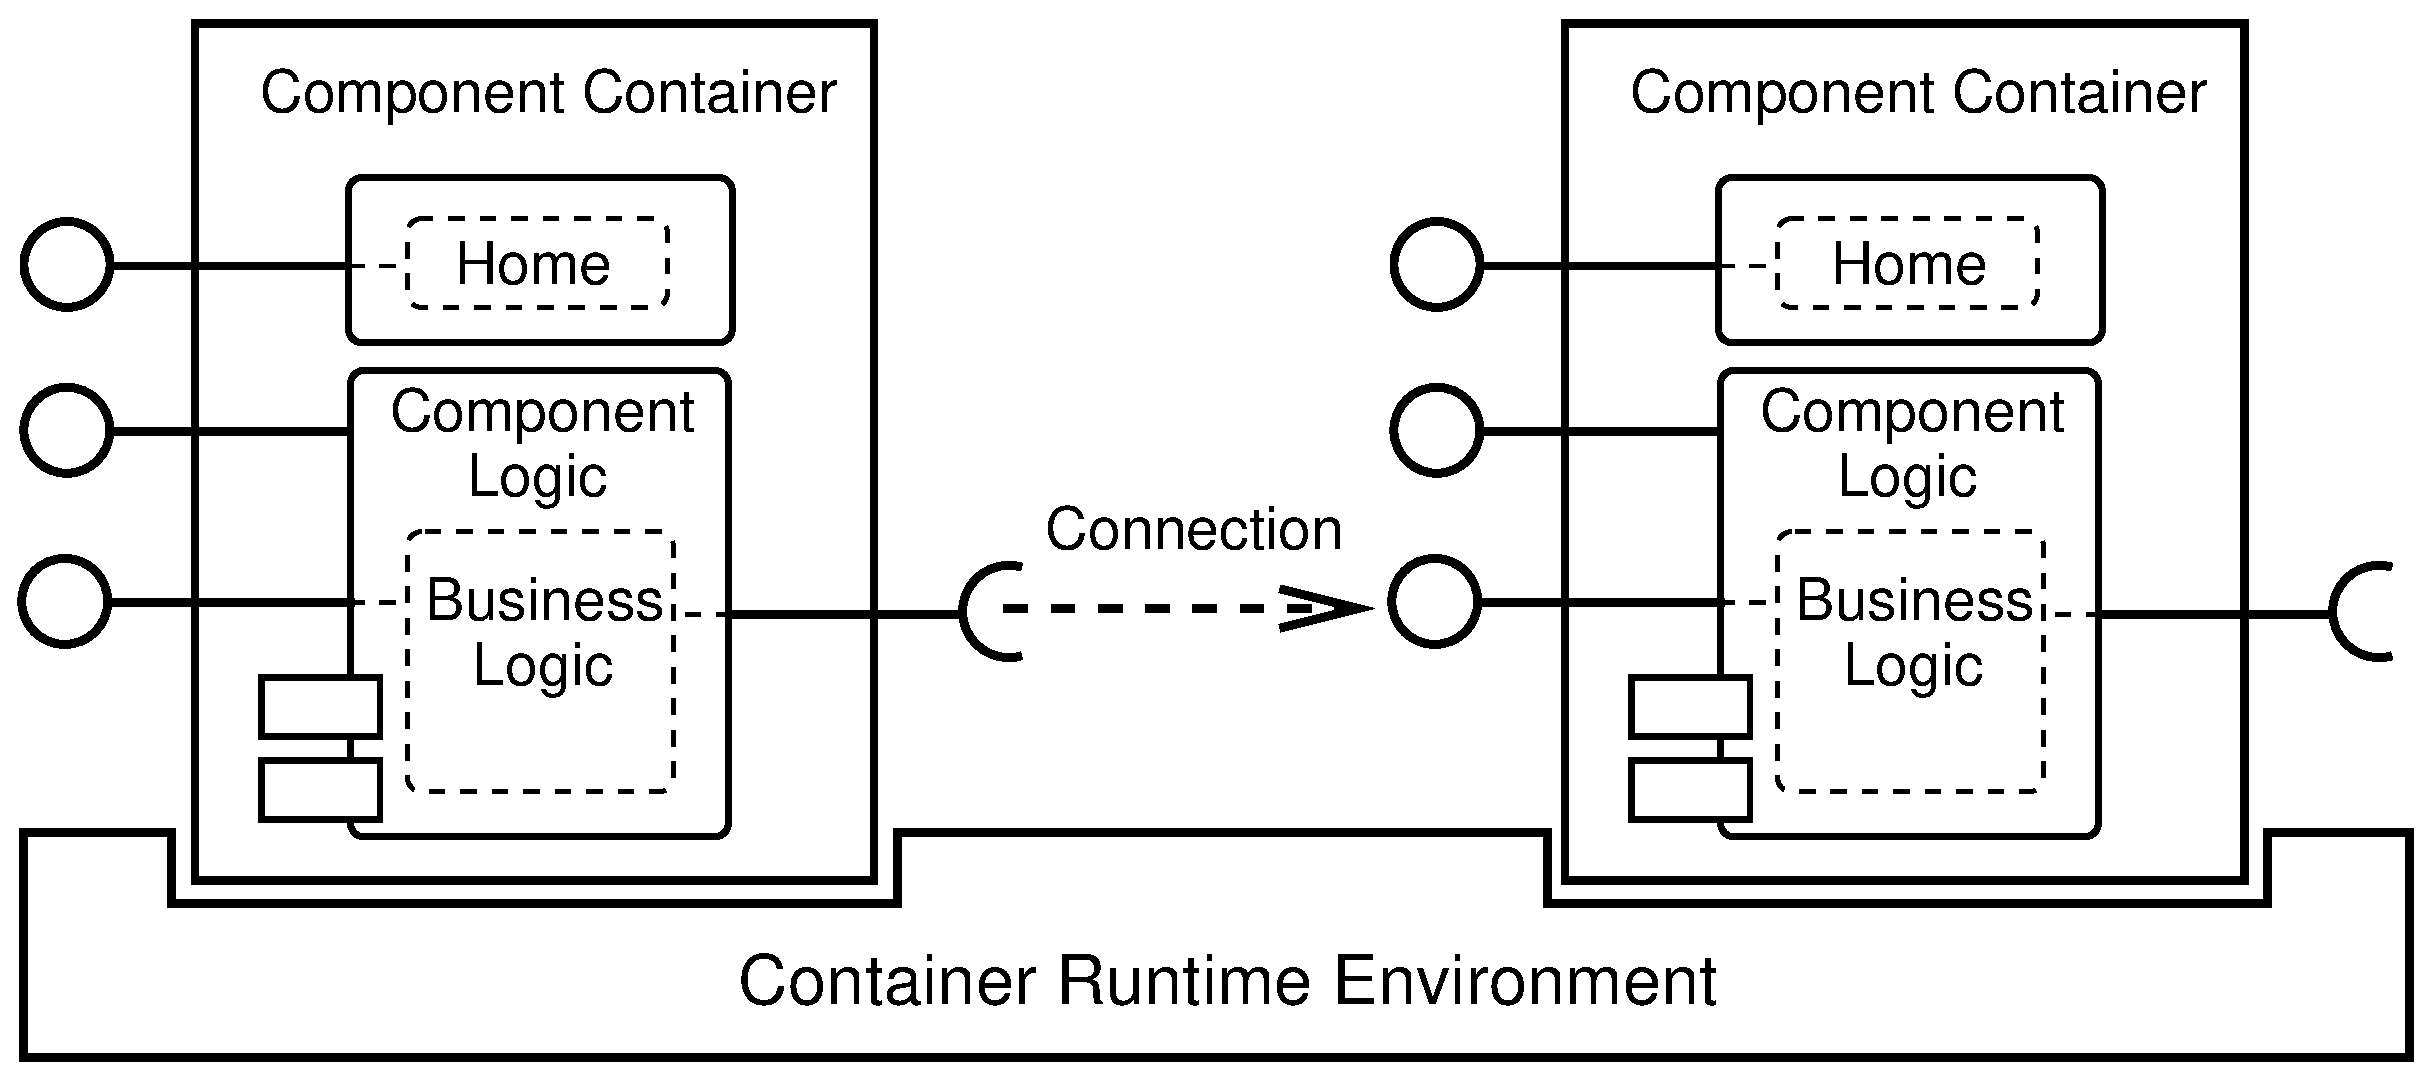
\includegraphics [width=10cm,angle=0] 
		     {ComponentModel/figures/ContainerComponentlogicBusinesslogic}
    \caption{A component implementation covers business logic, component
    logic, component container and container runtime environment.}
    \label{ContainerComponentlogicBusinesslogic}            
    \end{center}
\end{figure}

\begin{description}
\item [Business logic:]
  a component's business logic is written by the component developer to 
  implement   a domain specific functionality.
  Basically, business logic should not deal with technical aspects like contract
  verification or middleware API.
  
\item [Component logic:]
  business logic is embedded in a layer of generated code called component 
  logic. The interaction between business logic and component logic is well 
  defined in terms of interfaces (context interface, callback interface).
  Component logic handles technical aspects as well as a component's life-cycle.
  Additionally, component logic is glue code that fits a component into a 
  generic component container.
  
\item [Component container:]
  a component type is hosted by a component container that manages instances of
  that component type.
  While component logic is generated for each particular component type, the 
  component container is a generic part of the component platform.
  
\item [Container runtime environment:]
  a component platform also supports a set of libraries and services that can 
  be used by component containers.
  Any middleware used here is also part of this runtime environment.
\end{description}


\noindent
From this implementation schema, two different component views can be deduced:
\begin{description}
\item [External view:]
  a component provides its ports defined by interfaces. All 
  client calls to these ports are routed through the component container and 
  the generated component logic before business logic functionality is
  executed.
  
\item [Internal view:]
  a component's business logic can call methods on a context 
  object, which is part of generated component logic, and has to implement 
  a callback interface that allows the component container to handle the 
  component's life--cycle.
\end{description}


\noindent
Conforming with the concept of component model and 
middleware separation, we have implemented a local version of LwCCM components.
These local components host business logic and are completely independent 
from a particular middleware technology.

\begin{figure}[htbp]
    \begin{center}
    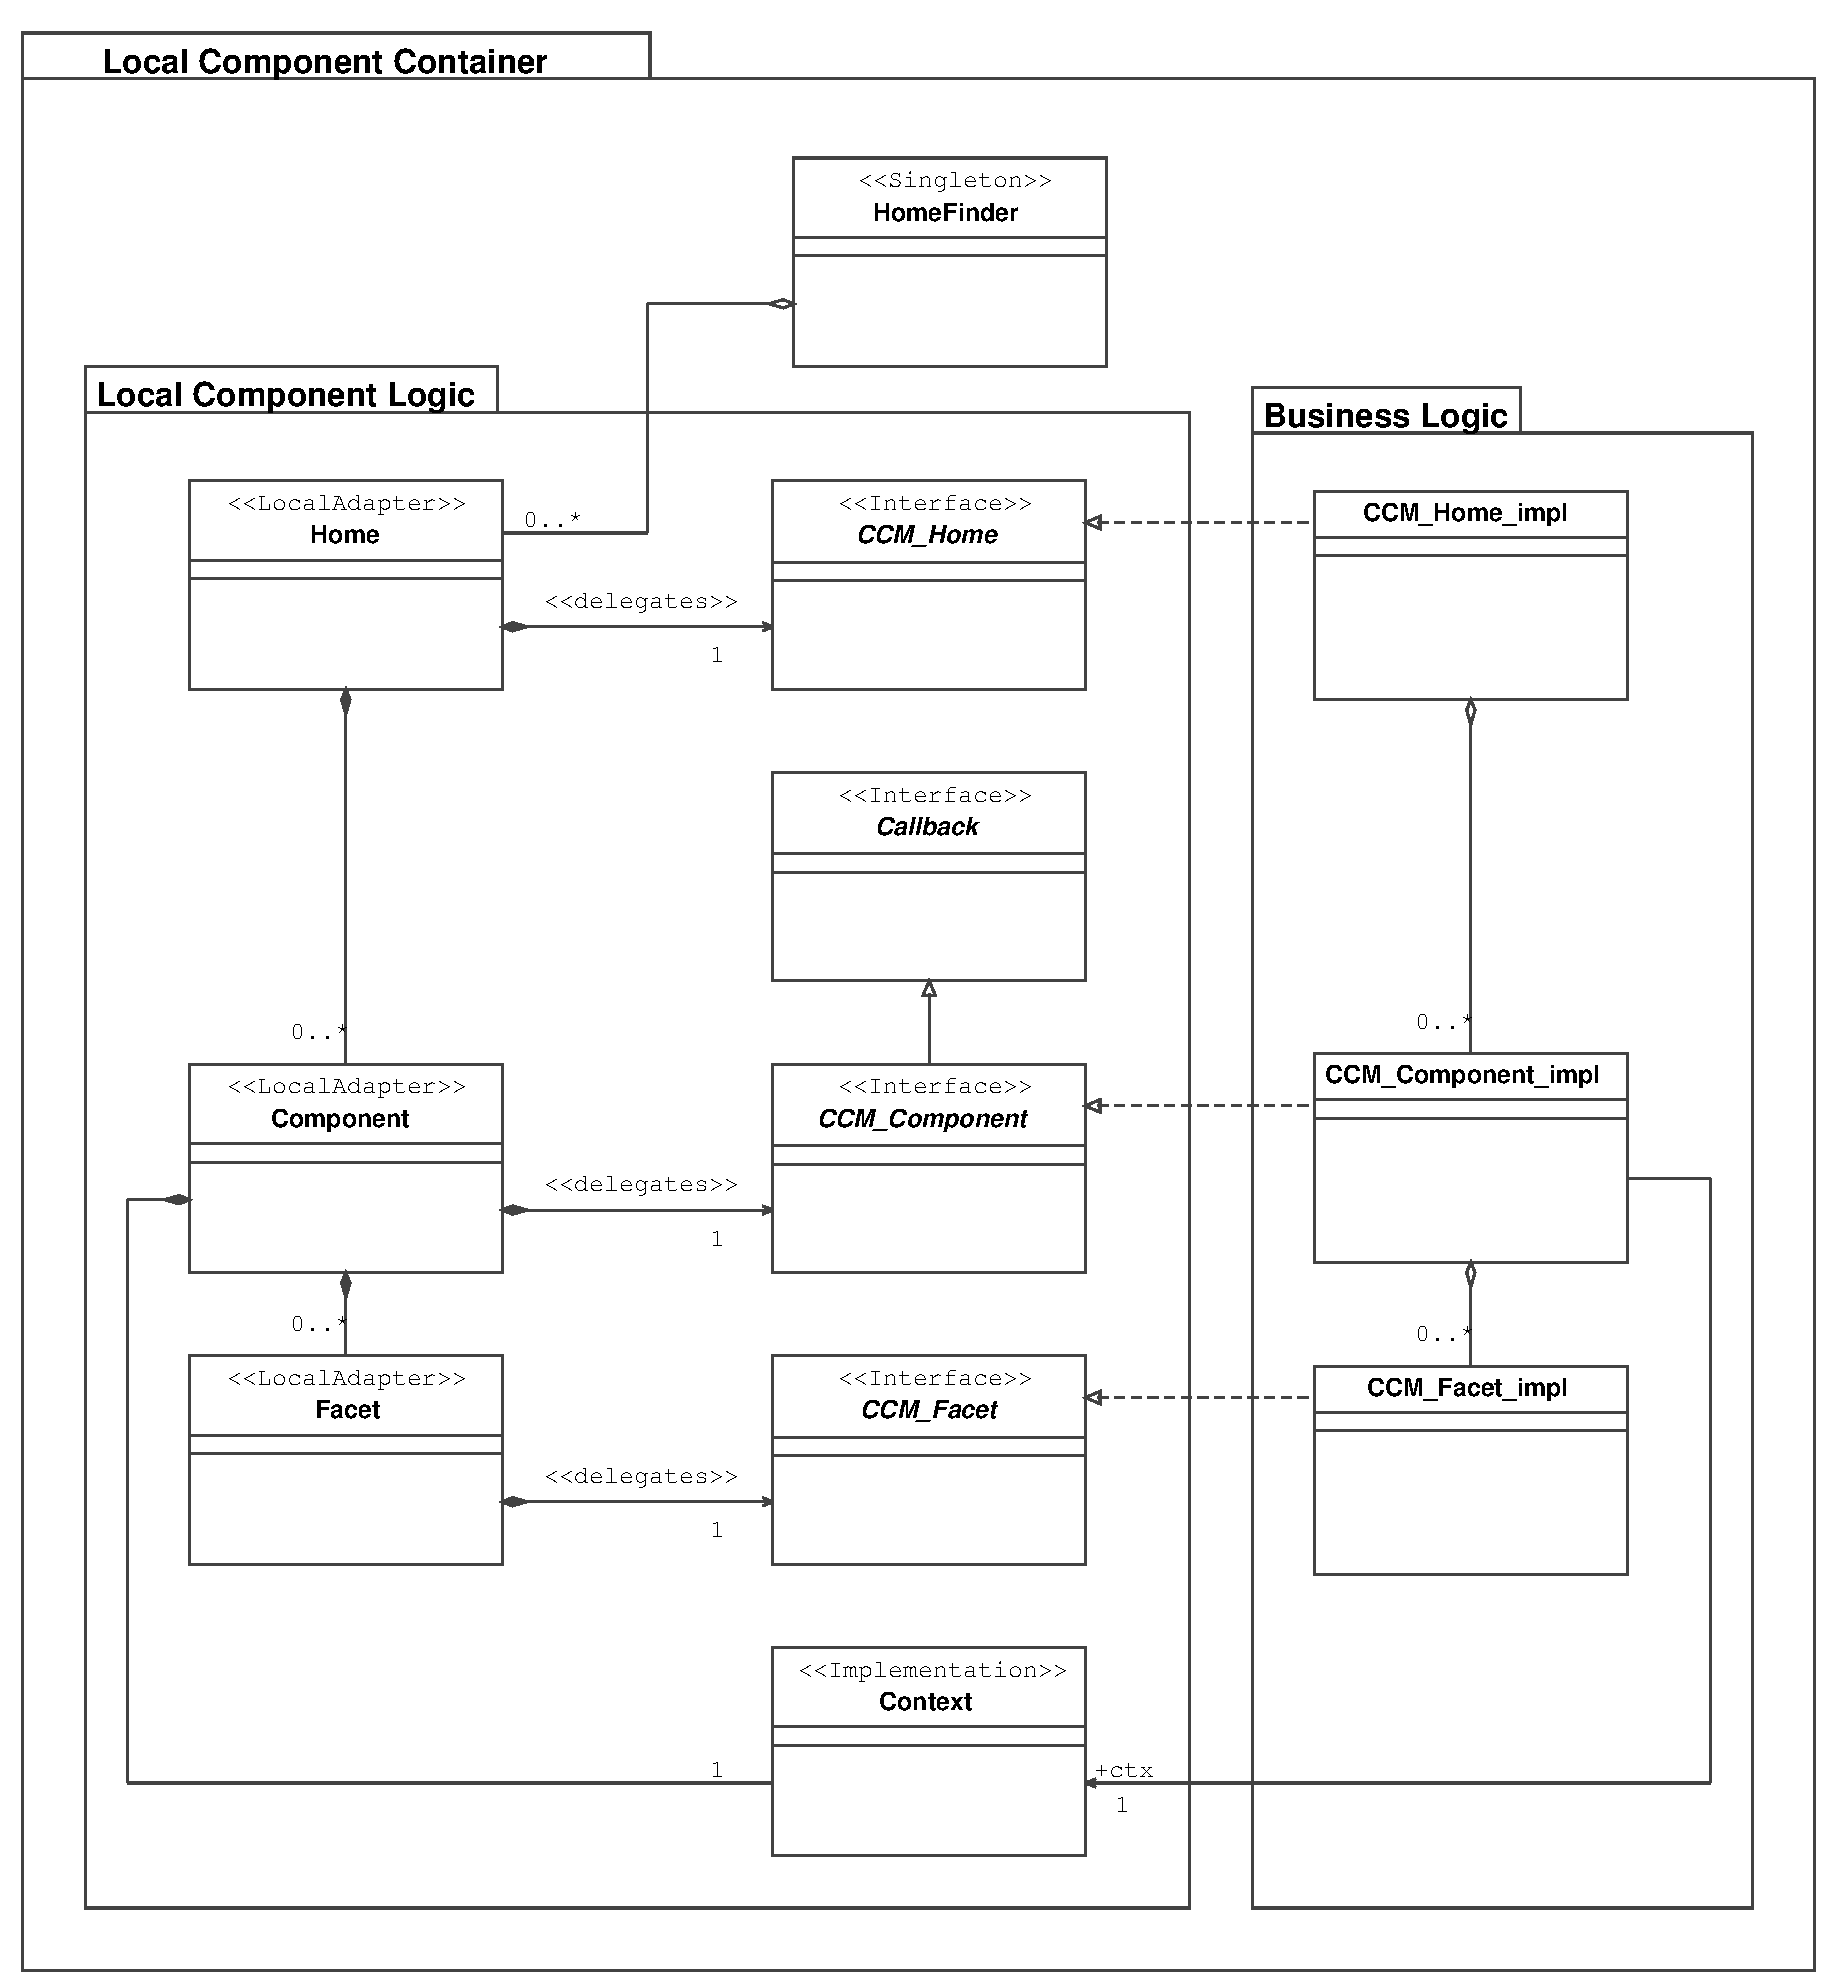
\includegraphics [width=15cm,angle=0] {ComponentModel/uml/StructureOfLocalComponents}
    \caption{This simplified structure of a local component implementation
    shows the relationship between business logic, local component logic and
    a local component container.}
    \label{StructureOfLocalComponents}            
    \end{center}
\end{figure}

\noindent
Implementations without middleware are much leaner and allow
finer grained components which are simpler to reuse.
Especially in languages that do not provide a native component model
(like C++), a local version of LwCCM can be useful.  

\newpage
\noindent
Based on this simplified class diagram, we can analyze the following
interactions between business logic and component logic:

\begin{description}
\item [Calling component methods:]
usually, a component client calls methods on a component's interface.
These interfaces can be either a component home, a component equivalent 
interface or a facet.
Invocations on all these interfaces follow the same structural pattern,
as shown in Fig.~\ref{LocalComponentImplementationStructure}.
A component's client calls methods on generated adapter classes 
that implements a component's interfaces. 
These adapters delegate calls 
to generated interfaces which are implemented by business logic classes.
\begin{figure}[htbp]
    \begin{center}
    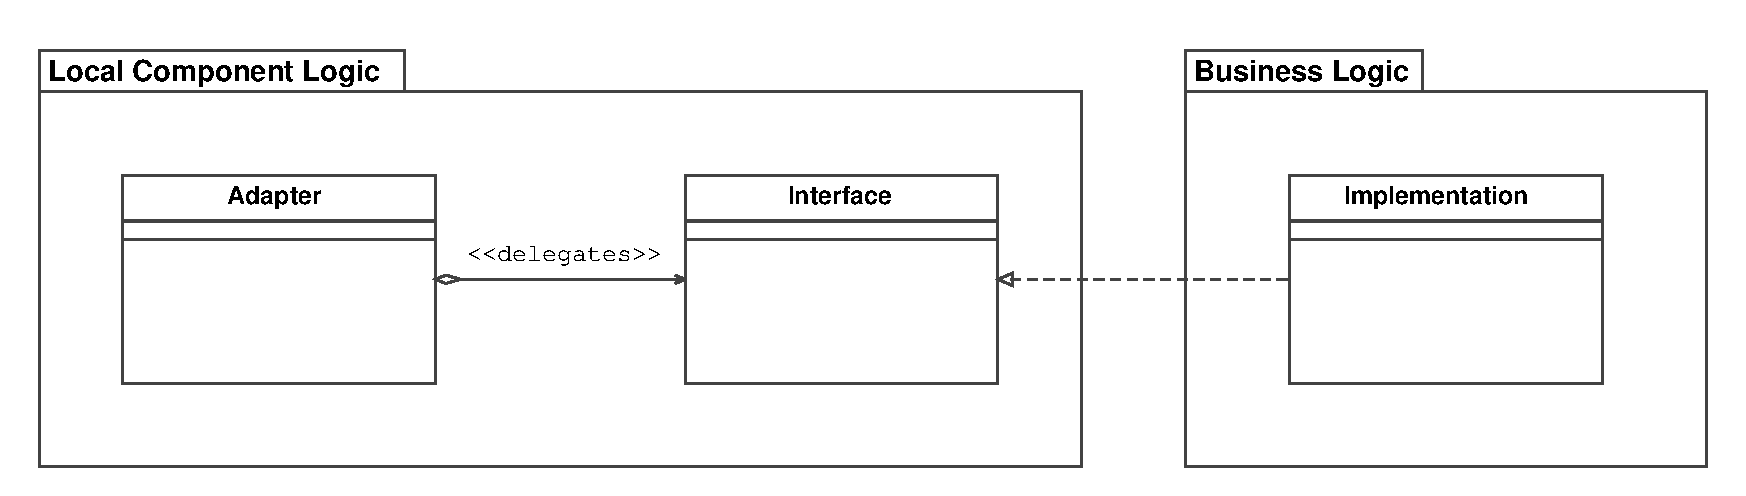
\includegraphics [width=13cm,angle=0] 
		     {ComponentModel/uml/LocalComponentImplementationStructure}
    \caption{Structure of a local component.}
    \label{LocalComponentImplementationStructure}            
    \end{center}
\end{figure}

This pattern implies two benefits:
\begin{itemize}
\item The adapter layer brings in an indirection that can be used to execute
some pre- and post-invocation functionality.  

\item Business logic can implement a well defined interface which is generated 
from the component model.
\end{itemize}

\item [Invoking callback methods:]
as shown in Fig.~\ref{StructureOfLocalComponents}, a generated component 
interface inherits the {\tt Callback} interface that defines methods which 
will be used by the component logic to control the business logic life-cycle.

\item [Using context methods:]
while calls from component clients as well as calls from component logic to 
the callback interface 
are directed from outside to the business logic, there is also
a need for interaction between business logic and generated glue code.

In the other direction, from business logic to component logic, a {\tt Context}
object is used to provide access to container functionality.
Additionally, business logic gets receptacle references from this context 
object, that are used to call methods defined by these receptacle interfaces.
Remember, receptacles are connected to facets which implement these common
interfaces.
\end{description}

\noindent
An important part of a local component container is the {\tt HomeFinder} class. 
This class is implemented as a singleton
\cite{Gamma95} and manages component home instances.
When a local LwCCM component is deployed, an instance of the component's home
is created and registered by the {\tt HomeFinder} using a unique name. 
After that, the {\tt HomeFinder} can be used to retrieve home references by 
their name.

% $Id$ 
%==============================================================================
\section{Nested Component Composition}
\label{NestedComponentComposition}
%==============================================================================


\begin{figure}[htb]
    \begin{center}
    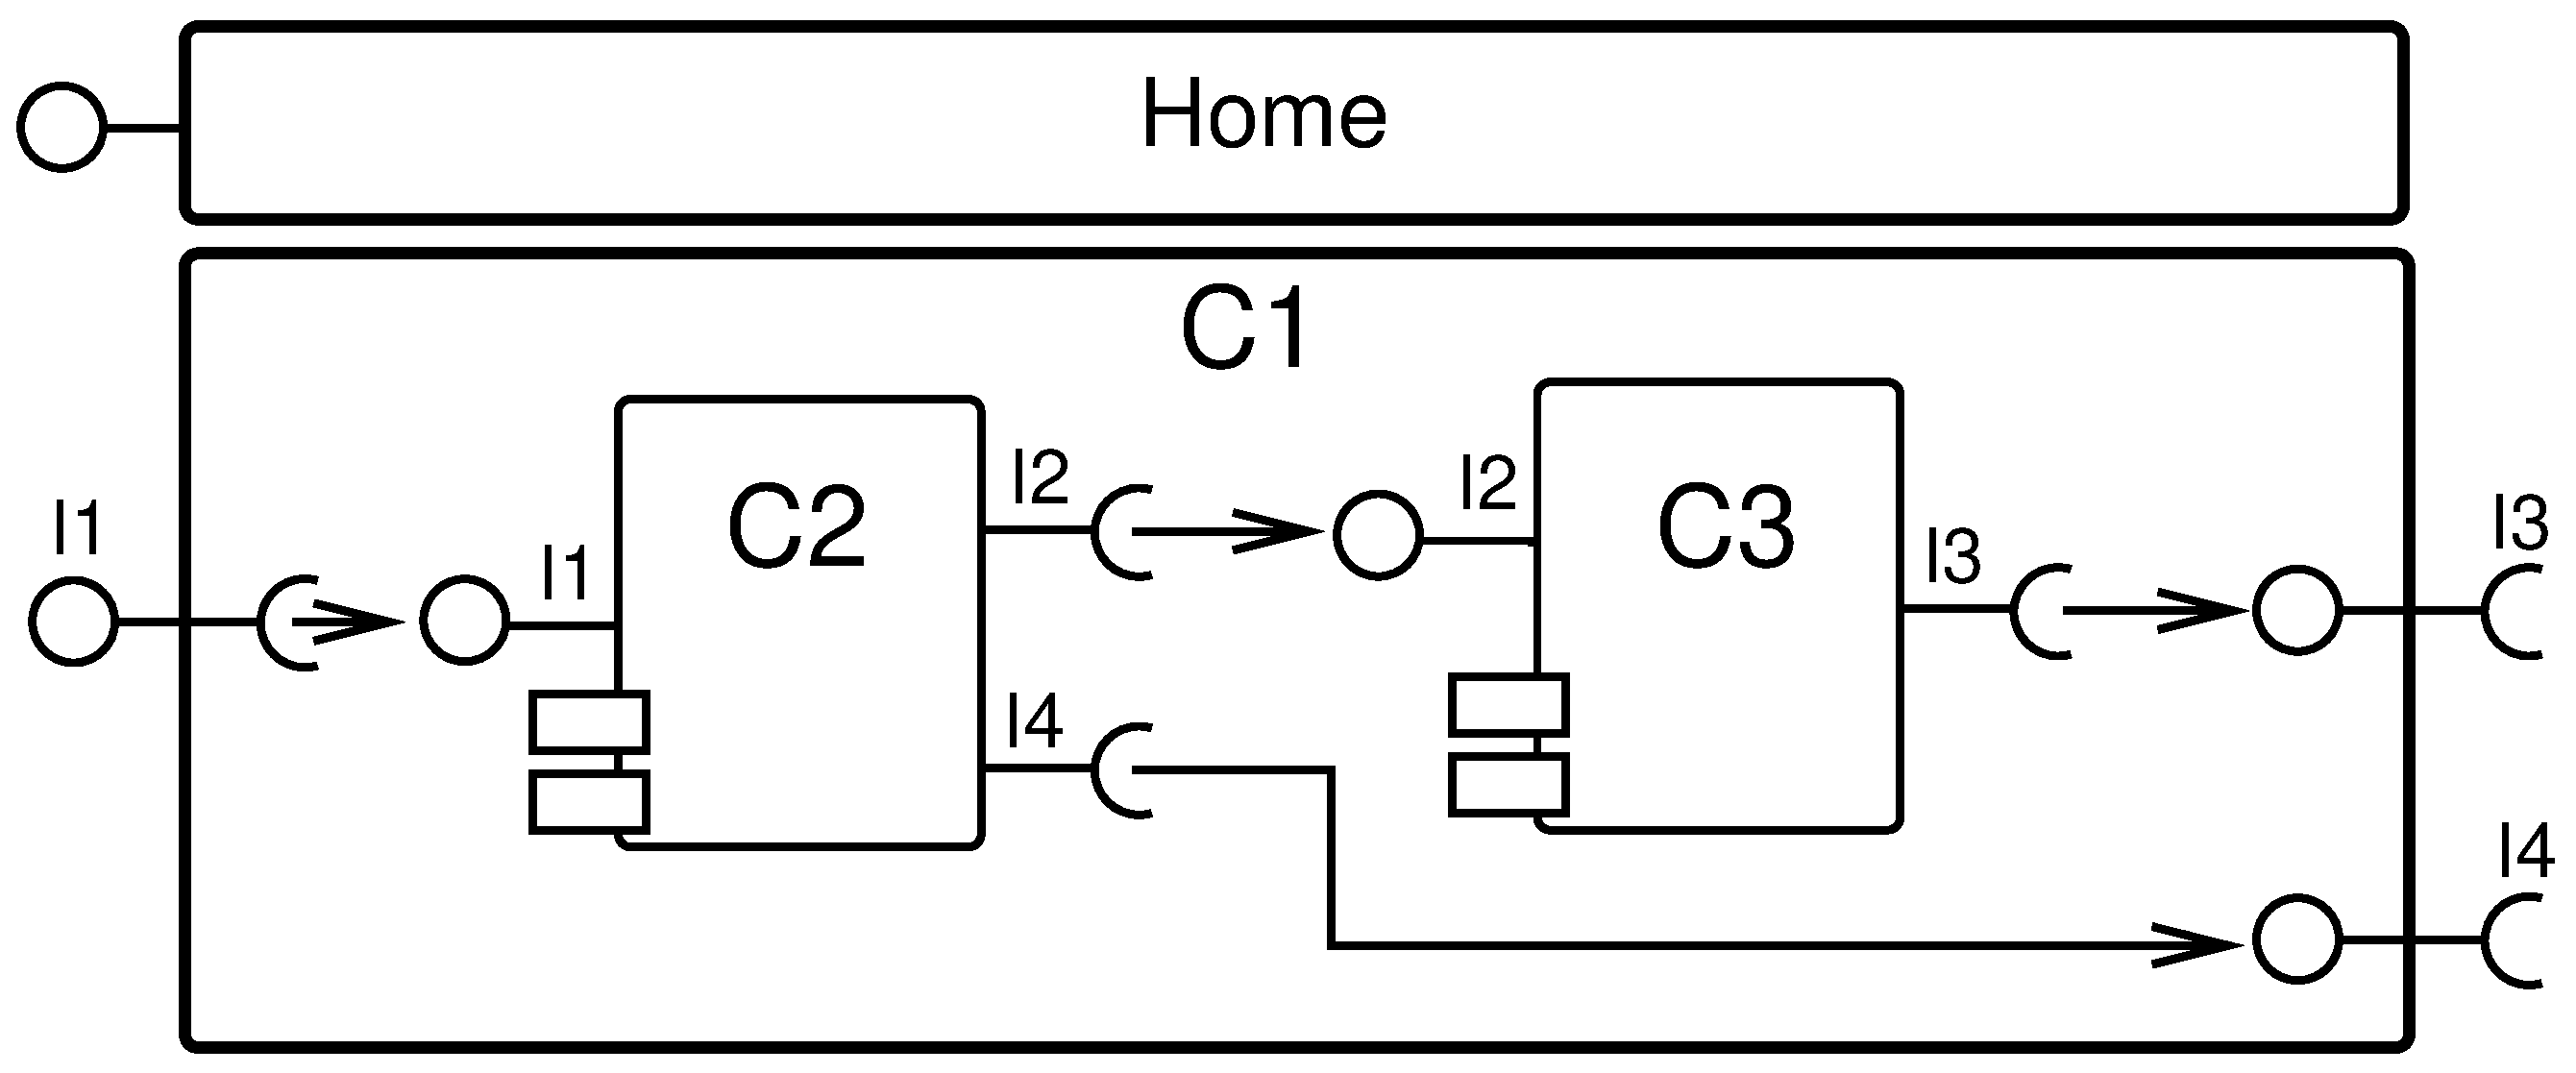
\includegraphics [width=7cm,angle=0] {ComponentModel/figures/NestedAssembly}
    \caption{ $C_{Ref}$ super component example.}
    \label{NestedAssembly}
    \end{center}
\end{figure}

Using the session facade pattern \cite{J2EECorePatterns}, 
we are able reduce a nested component composition into a flat component 
assembly that can be described by a simple CAD file.
While the inner components $C2$, $C3$ keep unchanged, the outer component $C1$ 
must be transformed into a special LwCCM component - the facade component, 
as shown in Fig.~\ref{NestedToFlatAssembly}.

\begin{figure}[htb]
    \begin{center}
    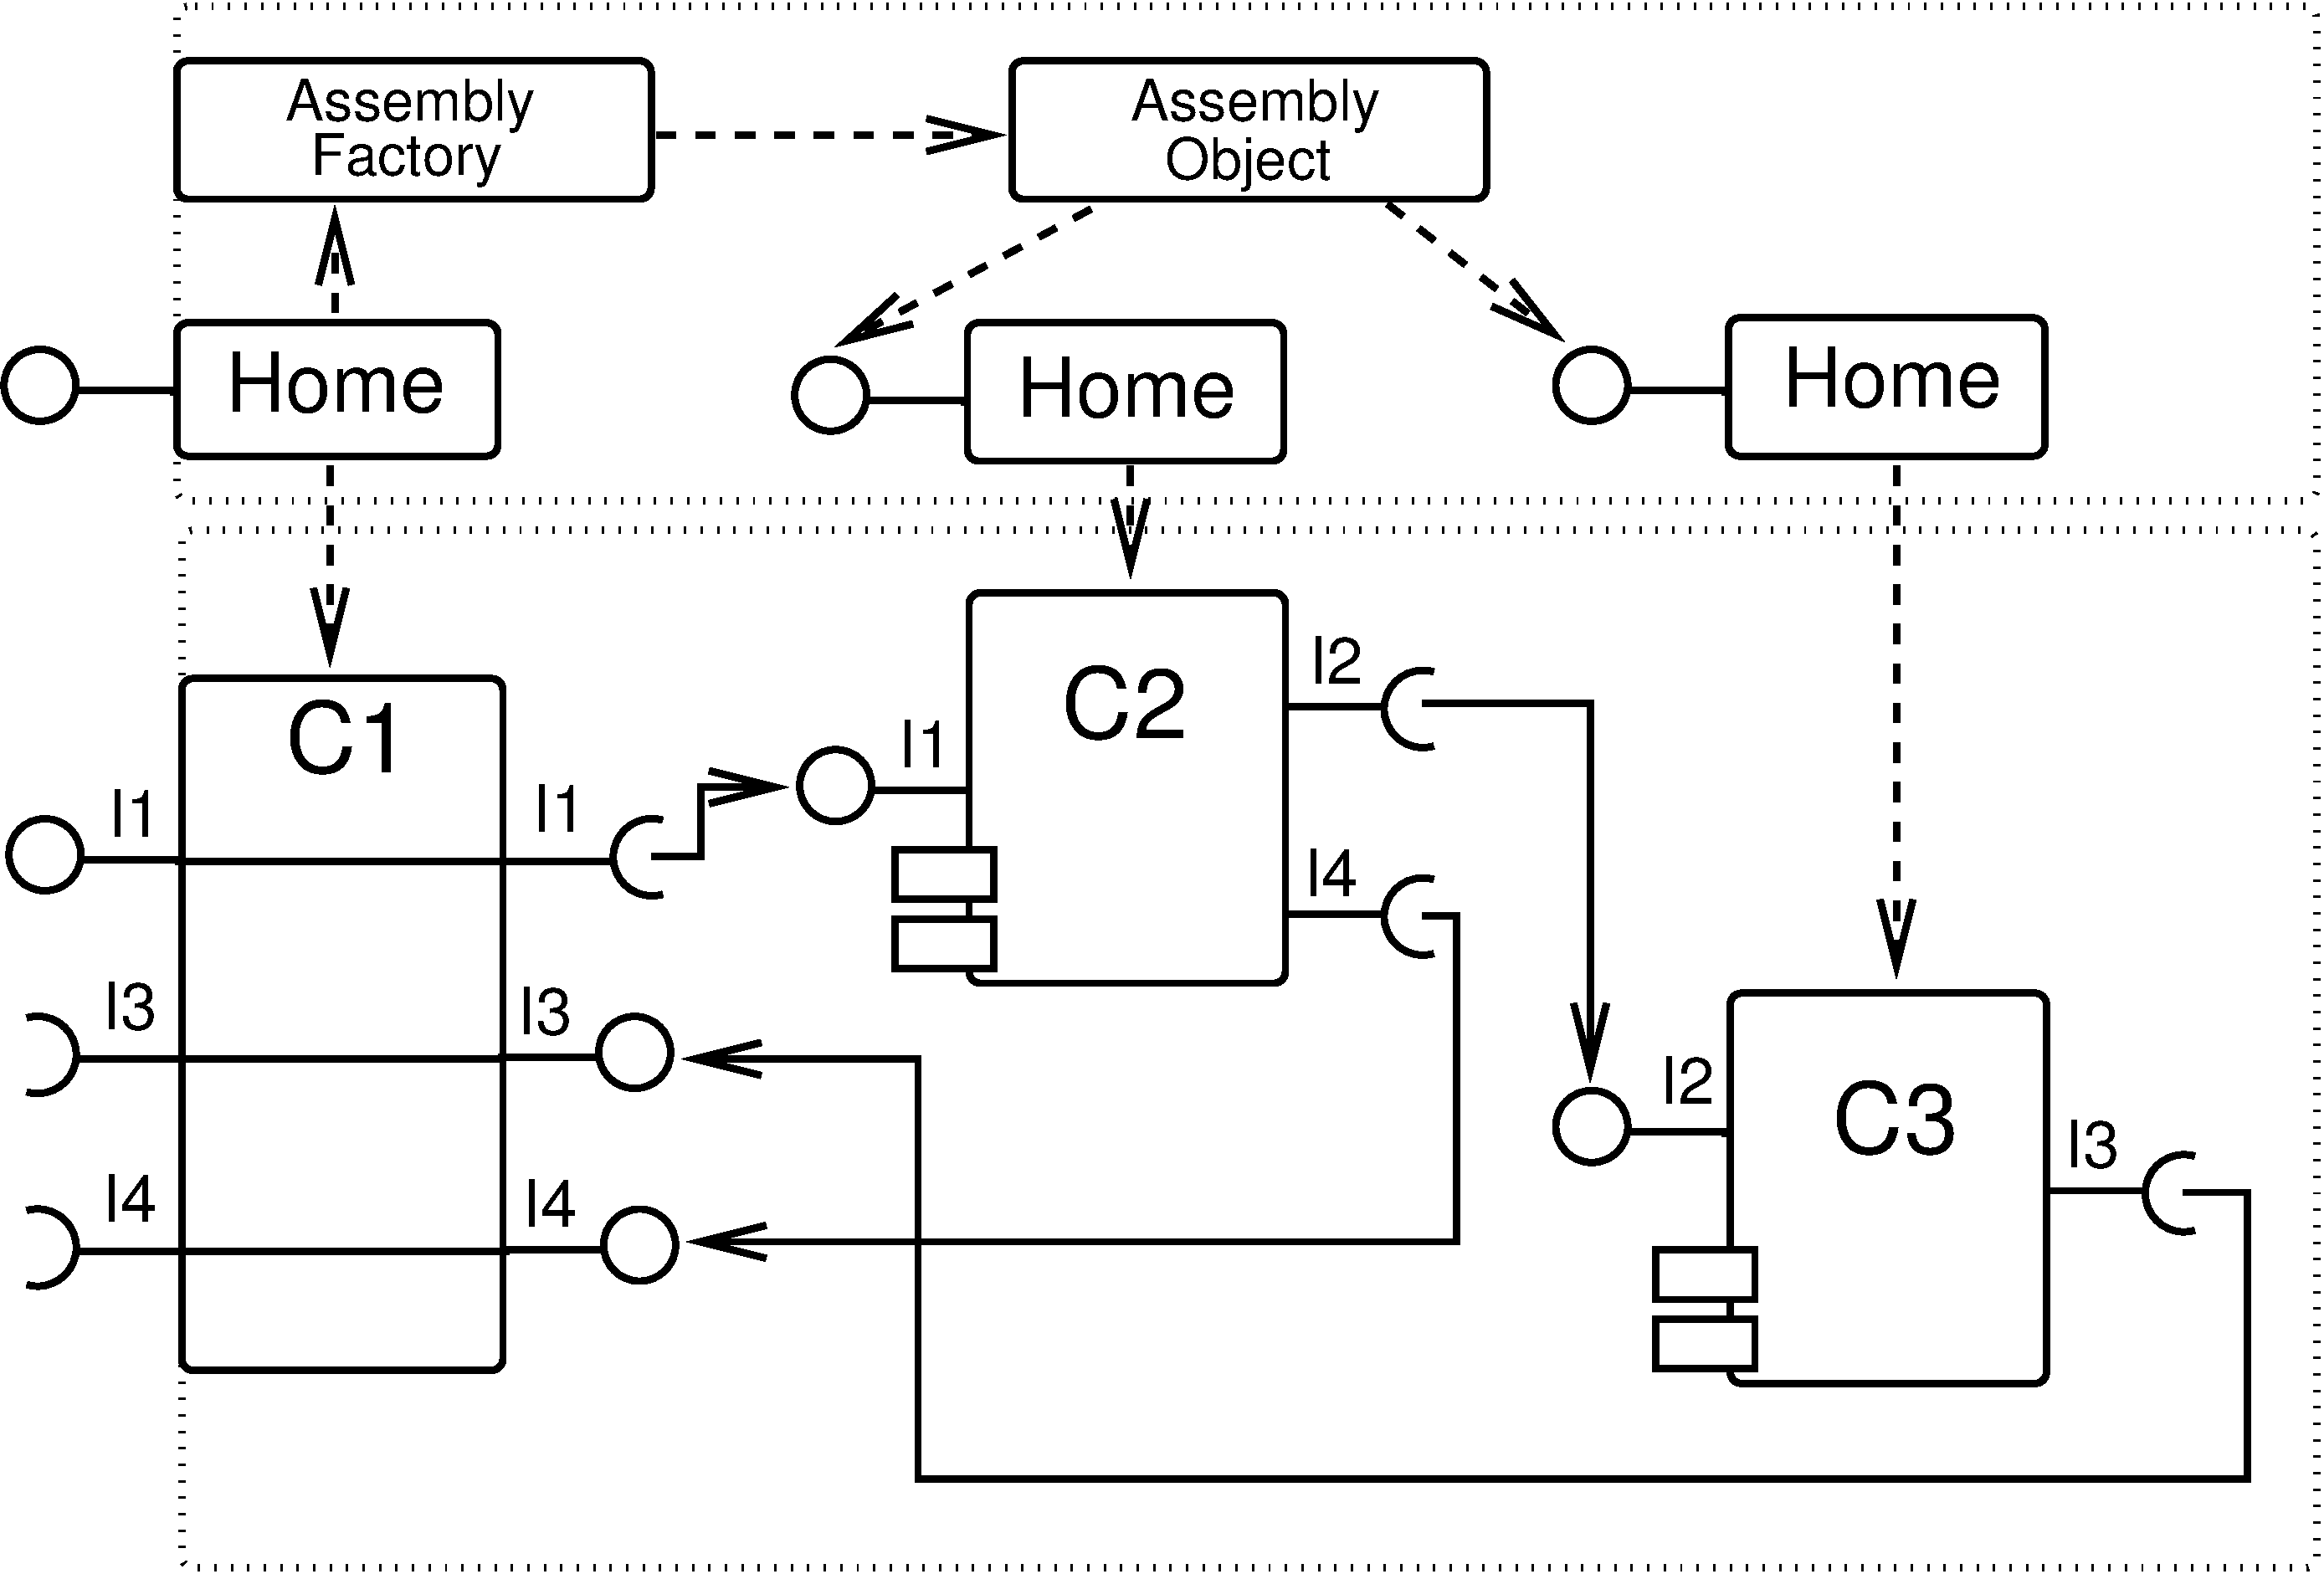
\includegraphics [width=7cm,angle=0] {ComponentModel/figures/NestedToFlatAssembly}
    \caption{Using the session facade pattern, a nested component composition
    can be reduced to a flat assembly as defined in LwCCM.}
    \label{NestedToFlatAssembly}
    \end{center}
\end{figure}

\noindent
The LwCCM facade component provides two complementary kinds of ports for each 
port defined in $C1$:
\begin{itemize}
\item {\bf Public ports.} A public port is visible to component clients and
can be accessed as a regular LwCCM component port.
 
\item {\bf Private ports.} A private port is a LwCCM port that is
not visible to component clients.
Private ports are used to connect the facade component with their inner 
component instances.
Technically, private ports are implemented like public ports, but after the
configuration phase, private ports can not be accessed by component clients. 
\end{itemize}
 
\noindent
All information about components and their connections within a super 
component are represented by an {\it Assembly Object}.
Such an assembly object is assigned to a facade component instance, and 
can be seen as a part of the facade component itself. 

For each facade component instance, an instance of the corresponding assembly
object must be created. 
To give a facade component's home the ability to create assembly object 
instances, an {\it Assembly Object Factory} must be assigned to a facade 
component home during component deployment.
With this approach, we can use regular LwCCM components and assemblies
to realize the nested component concept.

The implementation of a facade component's business logic is straightforward, 
each call to a facet method delegates to the corresponding receptacle and 
vice versa.

\vspace{3mm}
\noindent
To give a client the illusion of a single component, a facade component has to
handle some tasks behind the scenes. These are defined by the following 
sequence diagrams. 

\begin{figure}[htb]
    \begin{center}
    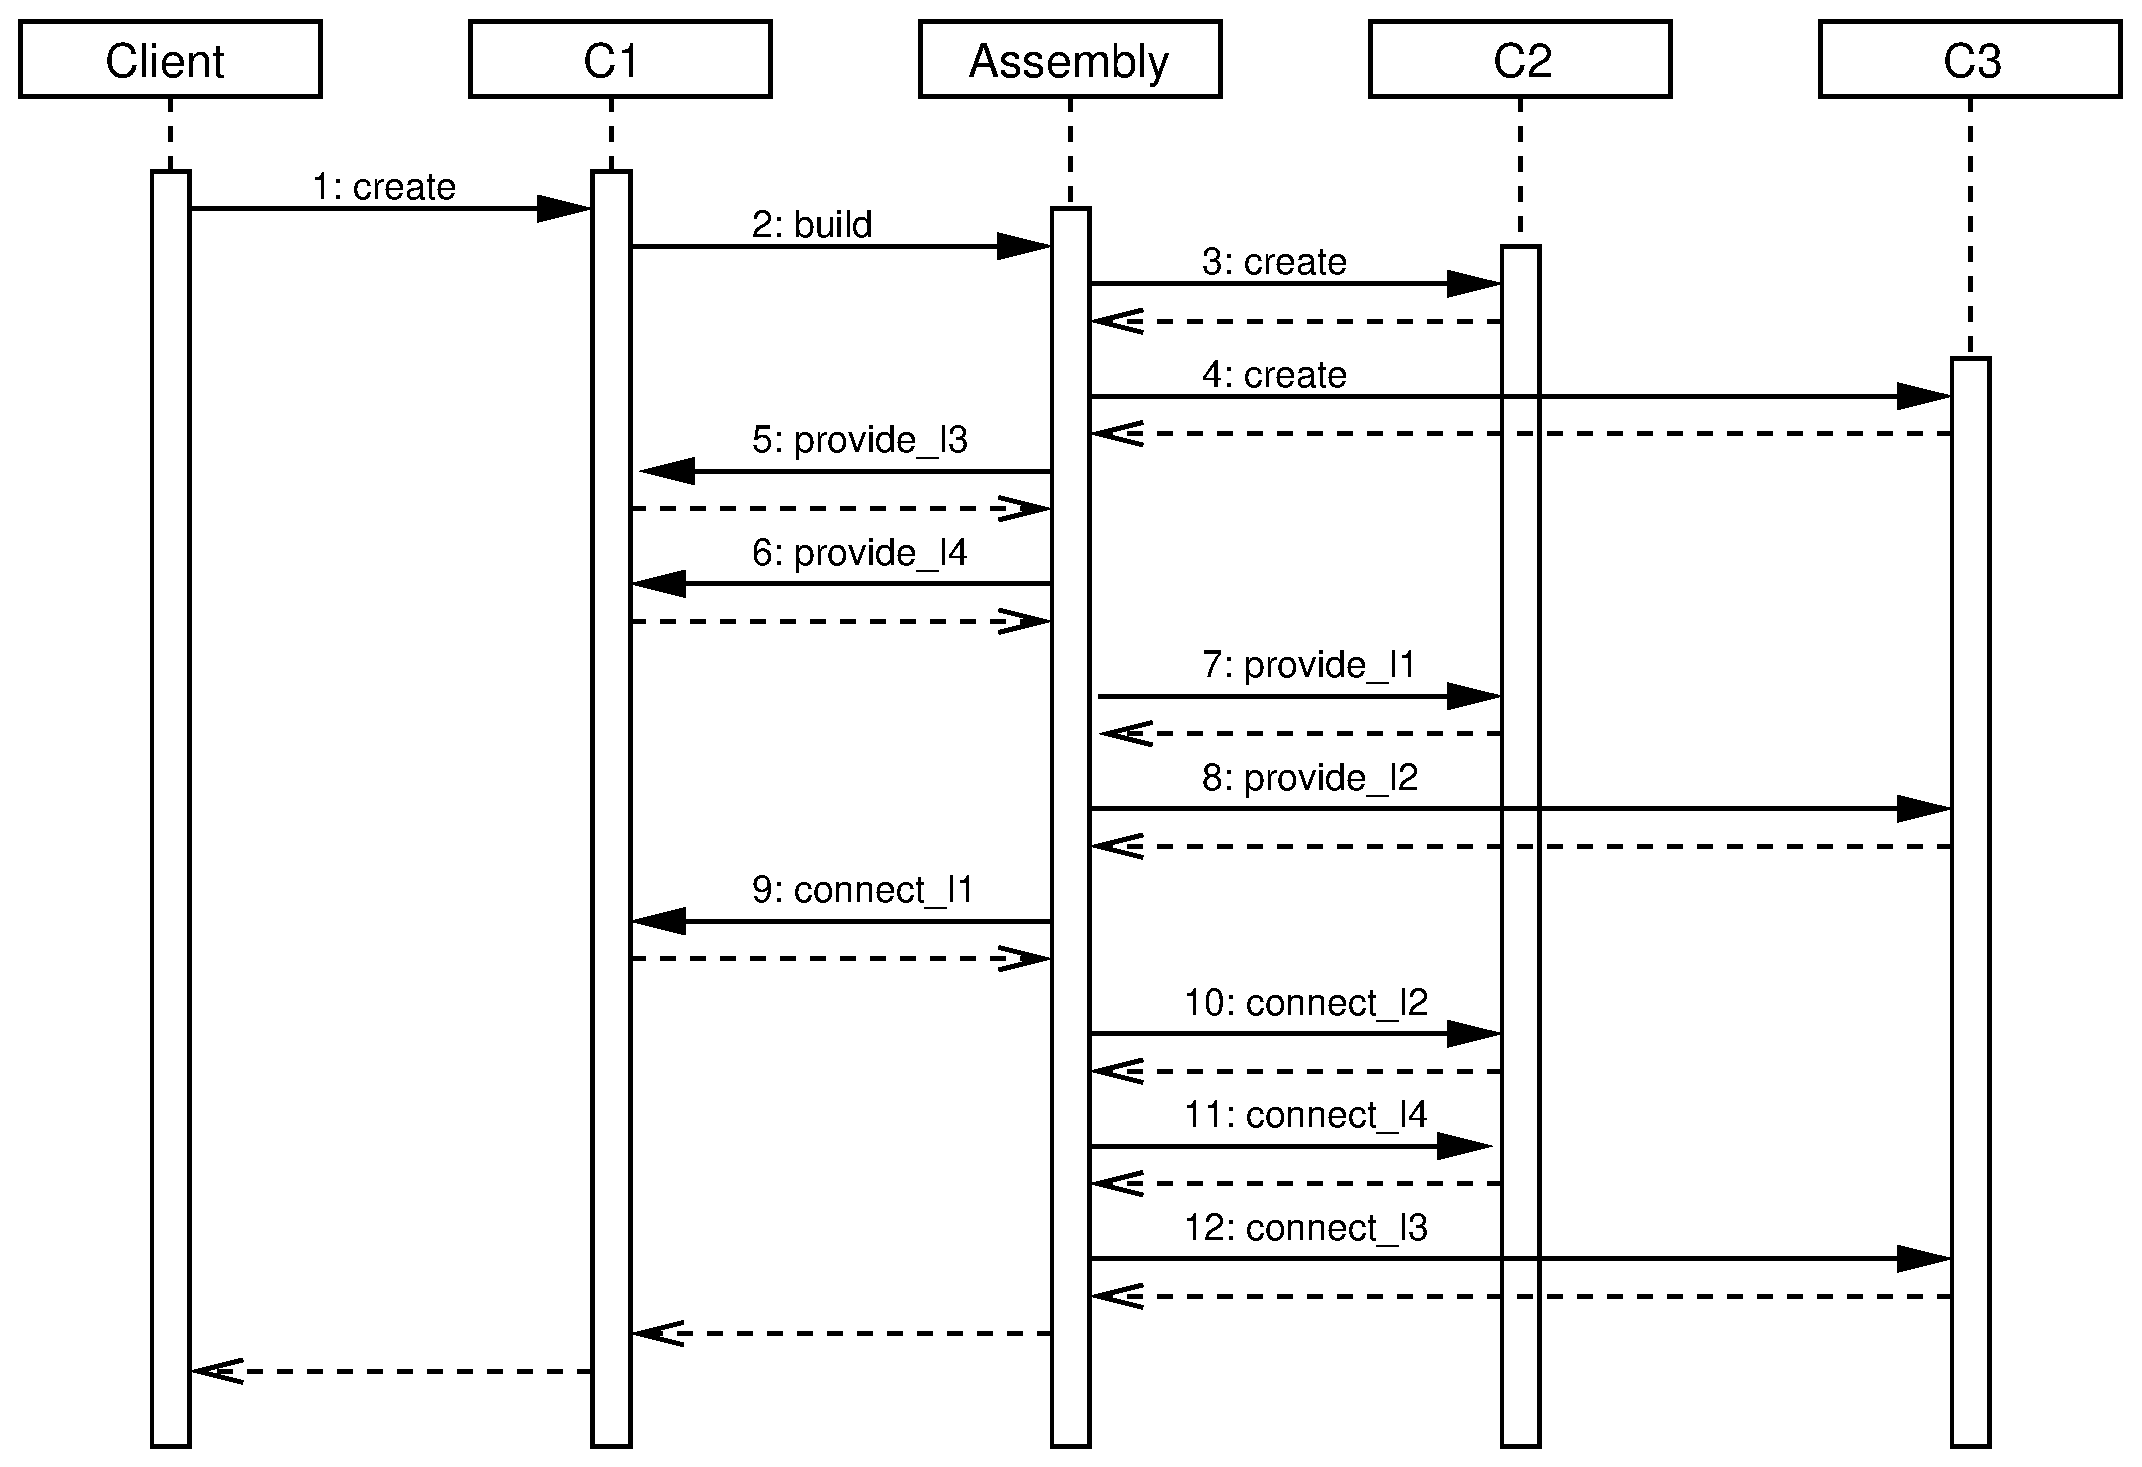
\includegraphics [width=12cm,angle=0] {ComponentModel/figures/SuperComponentCreate}
    \caption{Create a super component of Fig~\ref{NestedToFlatAssembly}.}
    \label{SuperComponentCreate}
    \end{center}
\end{figure}

\noindent
From a client's point of view, there is only one component $C_1$ that can be
instantiated by $C_1$'s home (Fig.~\ref{SuperComponentCreate}).
In fact, $C_1$ calls the {\tt build} method of the associated assembly object.
This assembly object in turn instantiates $C_2$ and $C_3$ and establishes all 
defined connections between these component instances.
After these activities, the assembly object returns to $C_1$ that finishes 
its create method.

Of course, $C_1$ itself can be part of another super component or connected 
to other components as well.
LwCCM defines the end of a component's configuration phase by calling the
{\tt configuration\_complete} method on each component instance.
In the case of a super component, this call must be delegated to all 
subcomponent instances (Fig.~\ref{SuperComponentConfigurationComplete}).
Before $C_1$ can return from {\tt configuration\_complete}, it has to lock all
private ports to prevent clients from directly accessing contained component 
instances.

\begin{figure}[htb]
    \begin{center}
    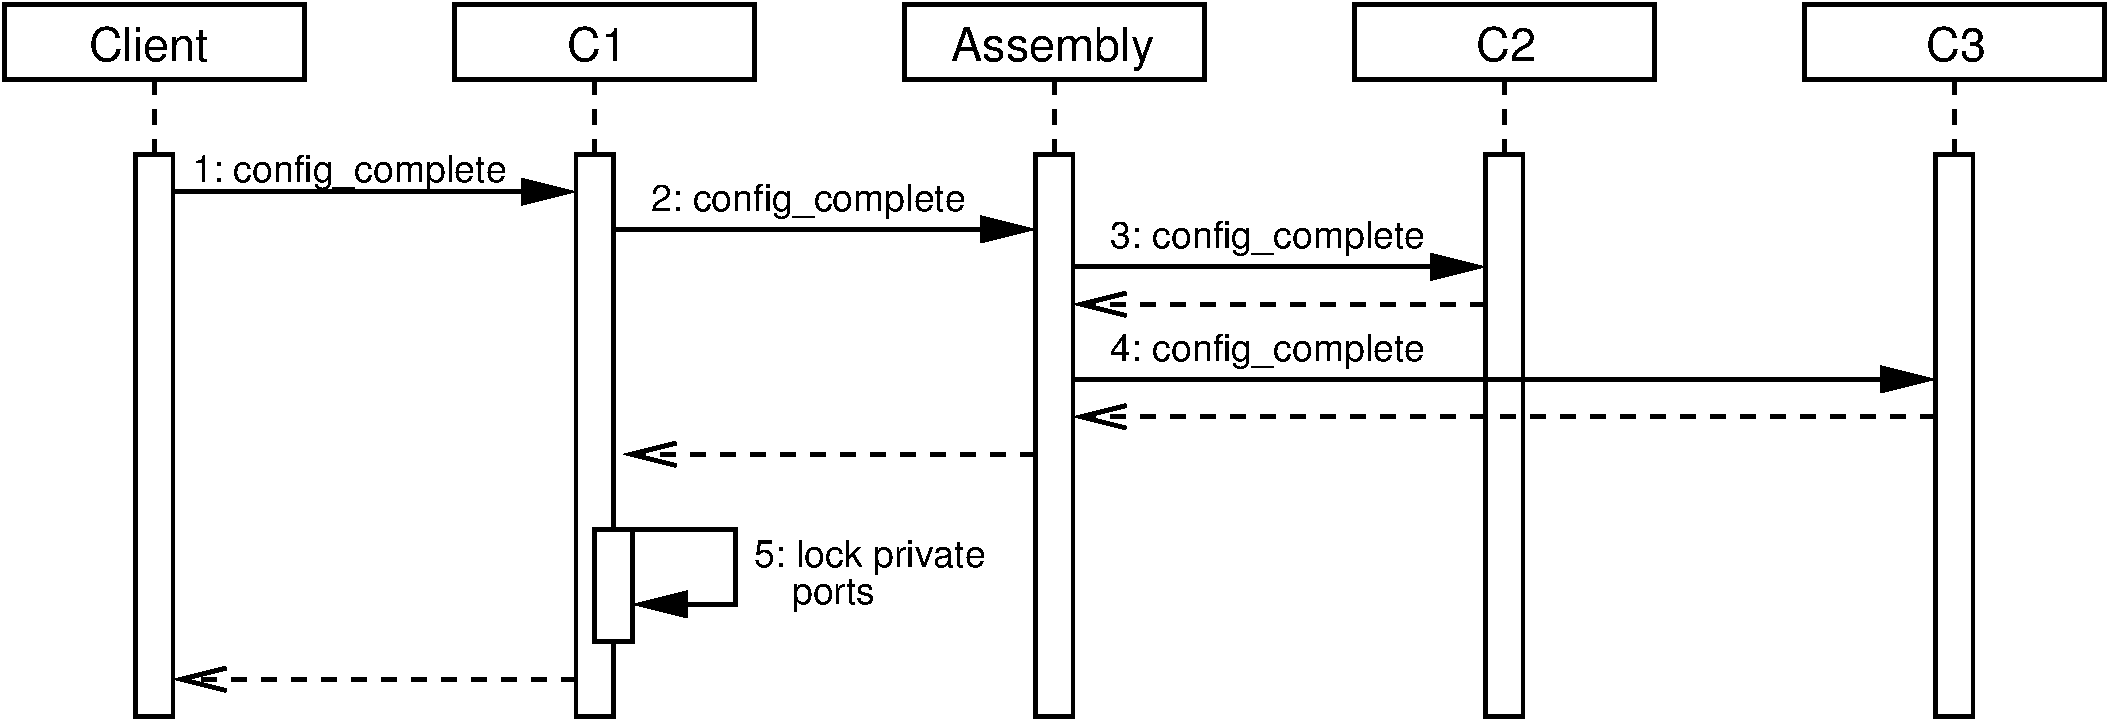
\includegraphics [width=12cm,angle=0] 
		     {ComponentModel/figures/SuperComponentConfigurationComplete}
    \caption{Completion of super component configuration phase.}
    \label{SuperComponentConfigurationComplete}
    \end{center}
\end{figure}

\noindent
Fig.~\ref{SuperComponentRemove} shows how a super component instance is removed:
$C_1$ triggers the assembly object to disconnect and destroy
all contained component instances.

\begin{figure}[htb]
    \begin{center}
    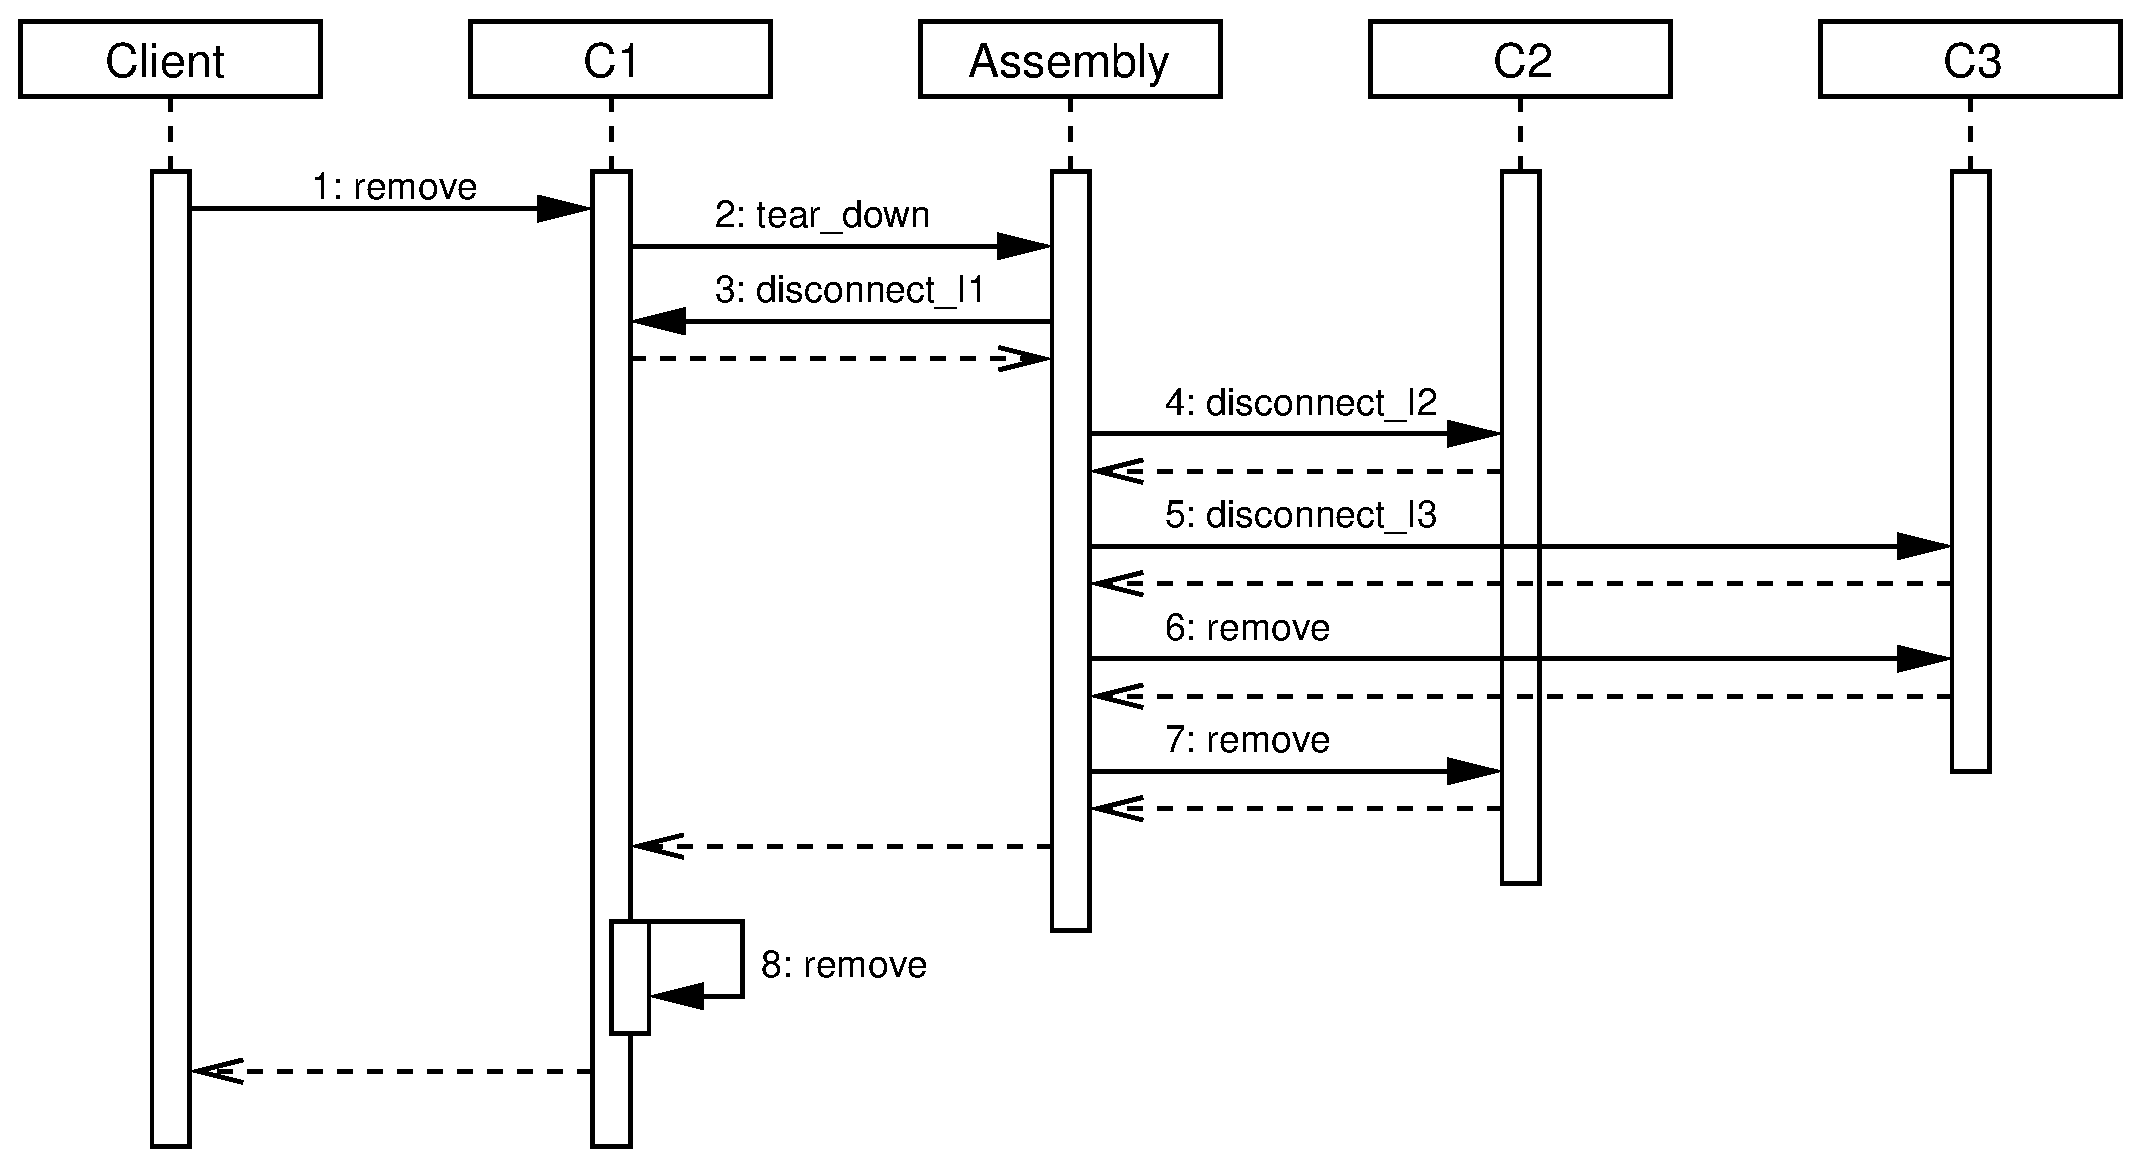
\includegraphics [width=12cm,angle=0] {ComponentModel/figures/SuperComponentRemove}
    \caption{Removal of a super component.}
    \label{SuperComponentRemove}
    \end{center}
\end{figure}

\noindent
A component client can handle
the super component in the same way as a regular LwCCM component.
Also, a simple LwCCM component can be seen as a special case of a super
component with an empty assembly.
Thus, both components and assemblies has been reduced to a single concept.


% $Id$

%==============================================================================
\section{Remote Component Structure}
%==============================================================================

While we have implemented a local version of CORBA Components, 
the LwCCM specification defines remote components only.
Remote components are built up from CORBA objects that implement defined
IDL interfaces.
Because of the specified mapping from IDL3 to IDL2, the generated IDL2 files 
can be processed by every existing IDL compiler. In addition to CORBA stubs
and skeletons, remote component logic as well as CORBA component containers
must be implemented too. 
To be compliant to the LwCCM specification, we have developed a way to
adapt local components into remote LwCCM components - the 
{\bf Local Component Adapter Concept} (LCAC).

LCAC allows to add remote communication
for each port transparently for business logic.
Fig.~\ref{LcacOverview} shows how a given local component implementation
can be extended to a remote LwCCM component.

\begin{figure}[htbp]
    \begin{center}
    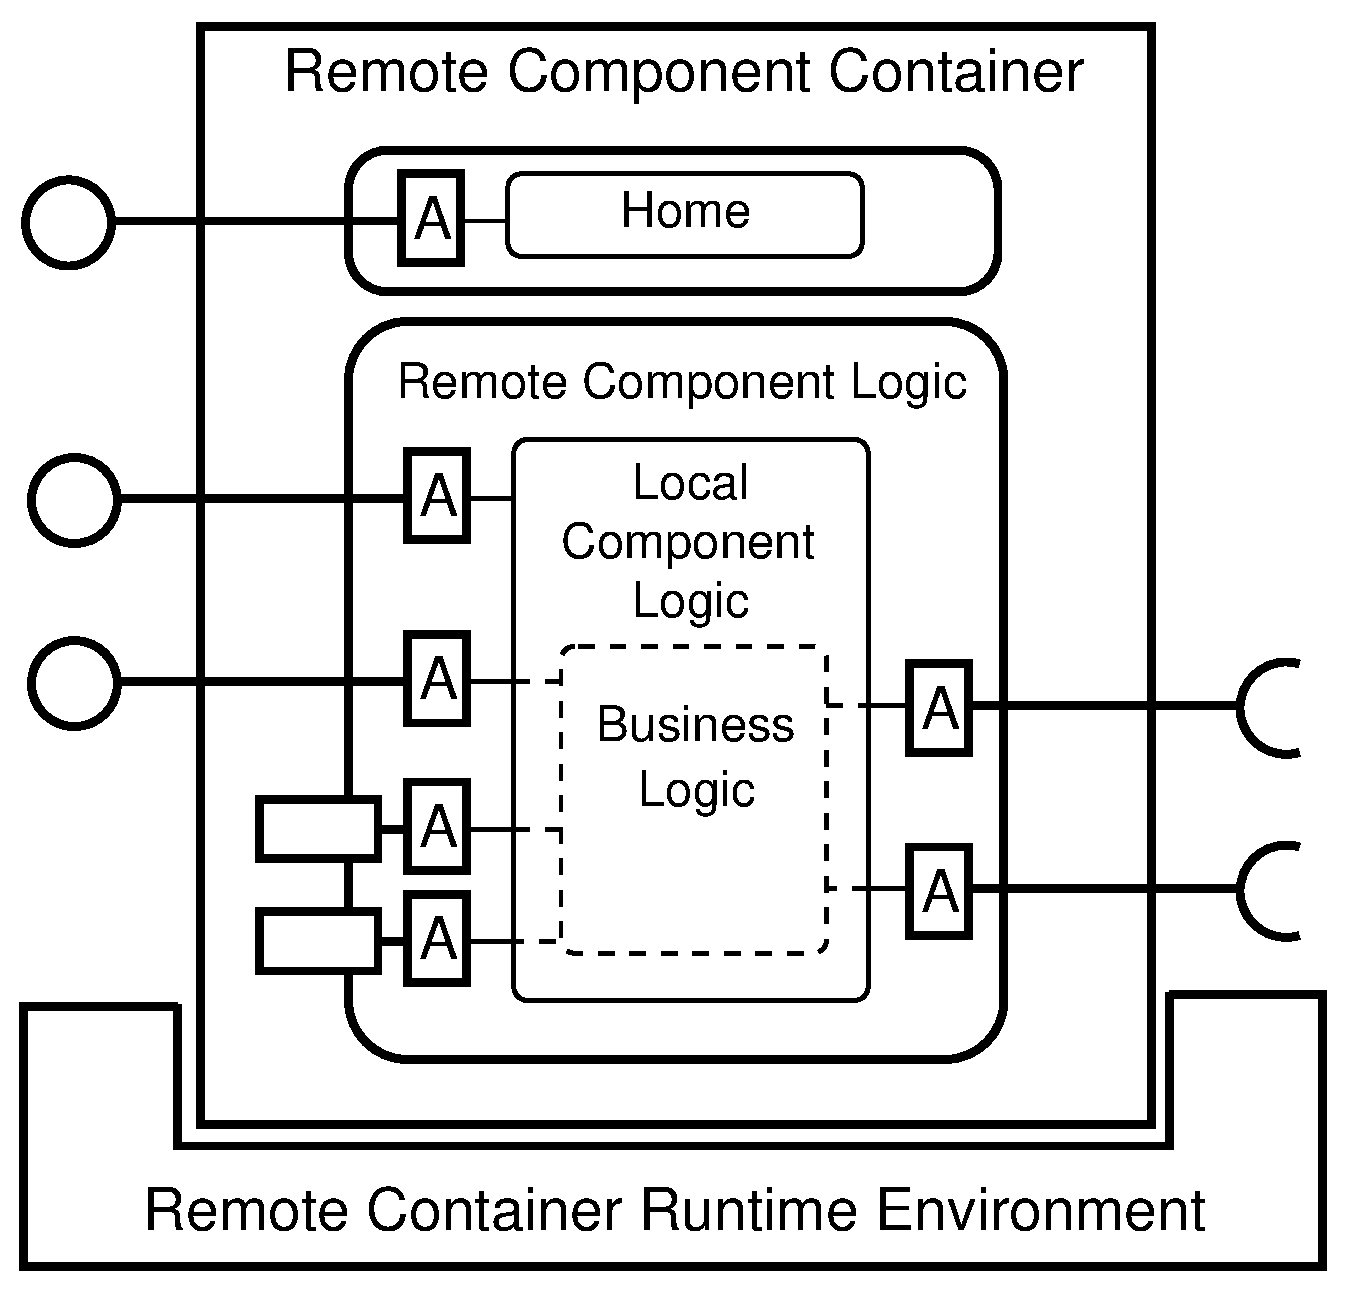
\includegraphics [width=5.5cm,angle=0] {figures/LocalAdapterConcept.eps}
    \caption{A local component can be embedded in a remote component logic
    that will be managed by a remote component container.}
    \label{LcacOverview}            
    \end{center}
\end{figure}

\noindent
The point is that we can use local components without changing them.
Thus, for a remote accessible component that provides at least one remote 
port, some additional code will be involved.

\begin{description}
\item [Remote component logic.]
A glue code layer is responsible for embedding a local component into a 
remote CORBA component. 
This remote component logic hosts a local component.
That means, its local component logic and business logic.  
Such a structure ensures that local ports can be used side by side to remote
ports.

\item [Adapter set.]
For a given IDL interface that defines a component port's syntax, a local and 
a remote implementation is generated. 
Using a set of adapter classes, these two worlds can fit together transparently.
In addition to component ports, adapters must be provided for component homes
as well as the component's equivalent interface.

\item [Remote component container.]
For each remote component type, a generic component container is used to
manage CORBA component instances.
In contrast to a local component container that can have a simple structure, a
remote container is also responsible for sophisticated {\it Quality of Service} 
(QoS) tasks.

\item [Remote container runtime environment.]
With increasing QoS functionality, the requirements to a remote container
runtime environment are growing too.
Besides an {\it Object Request Broker} (ORB), that handles CORBA requests,
libraries for multi--threading and process management implementation must 
be available.  
\end{description}

\noindent
This adapter concept is a powerful tool especially in heterogeneous 
environments. Besides the choice between local and remote connections, 
a deployment process can also decide to use different middleware technologies.


The fact that a local component is wrapped by a remote component becomes 
obvious from Fig.~\ref{StructureOfRemoteComponents}. All classes of a local
component remain unchanged, while some new ``remote'' classes have been added.

\begin{figure}[htbp]
    \begin{center}
    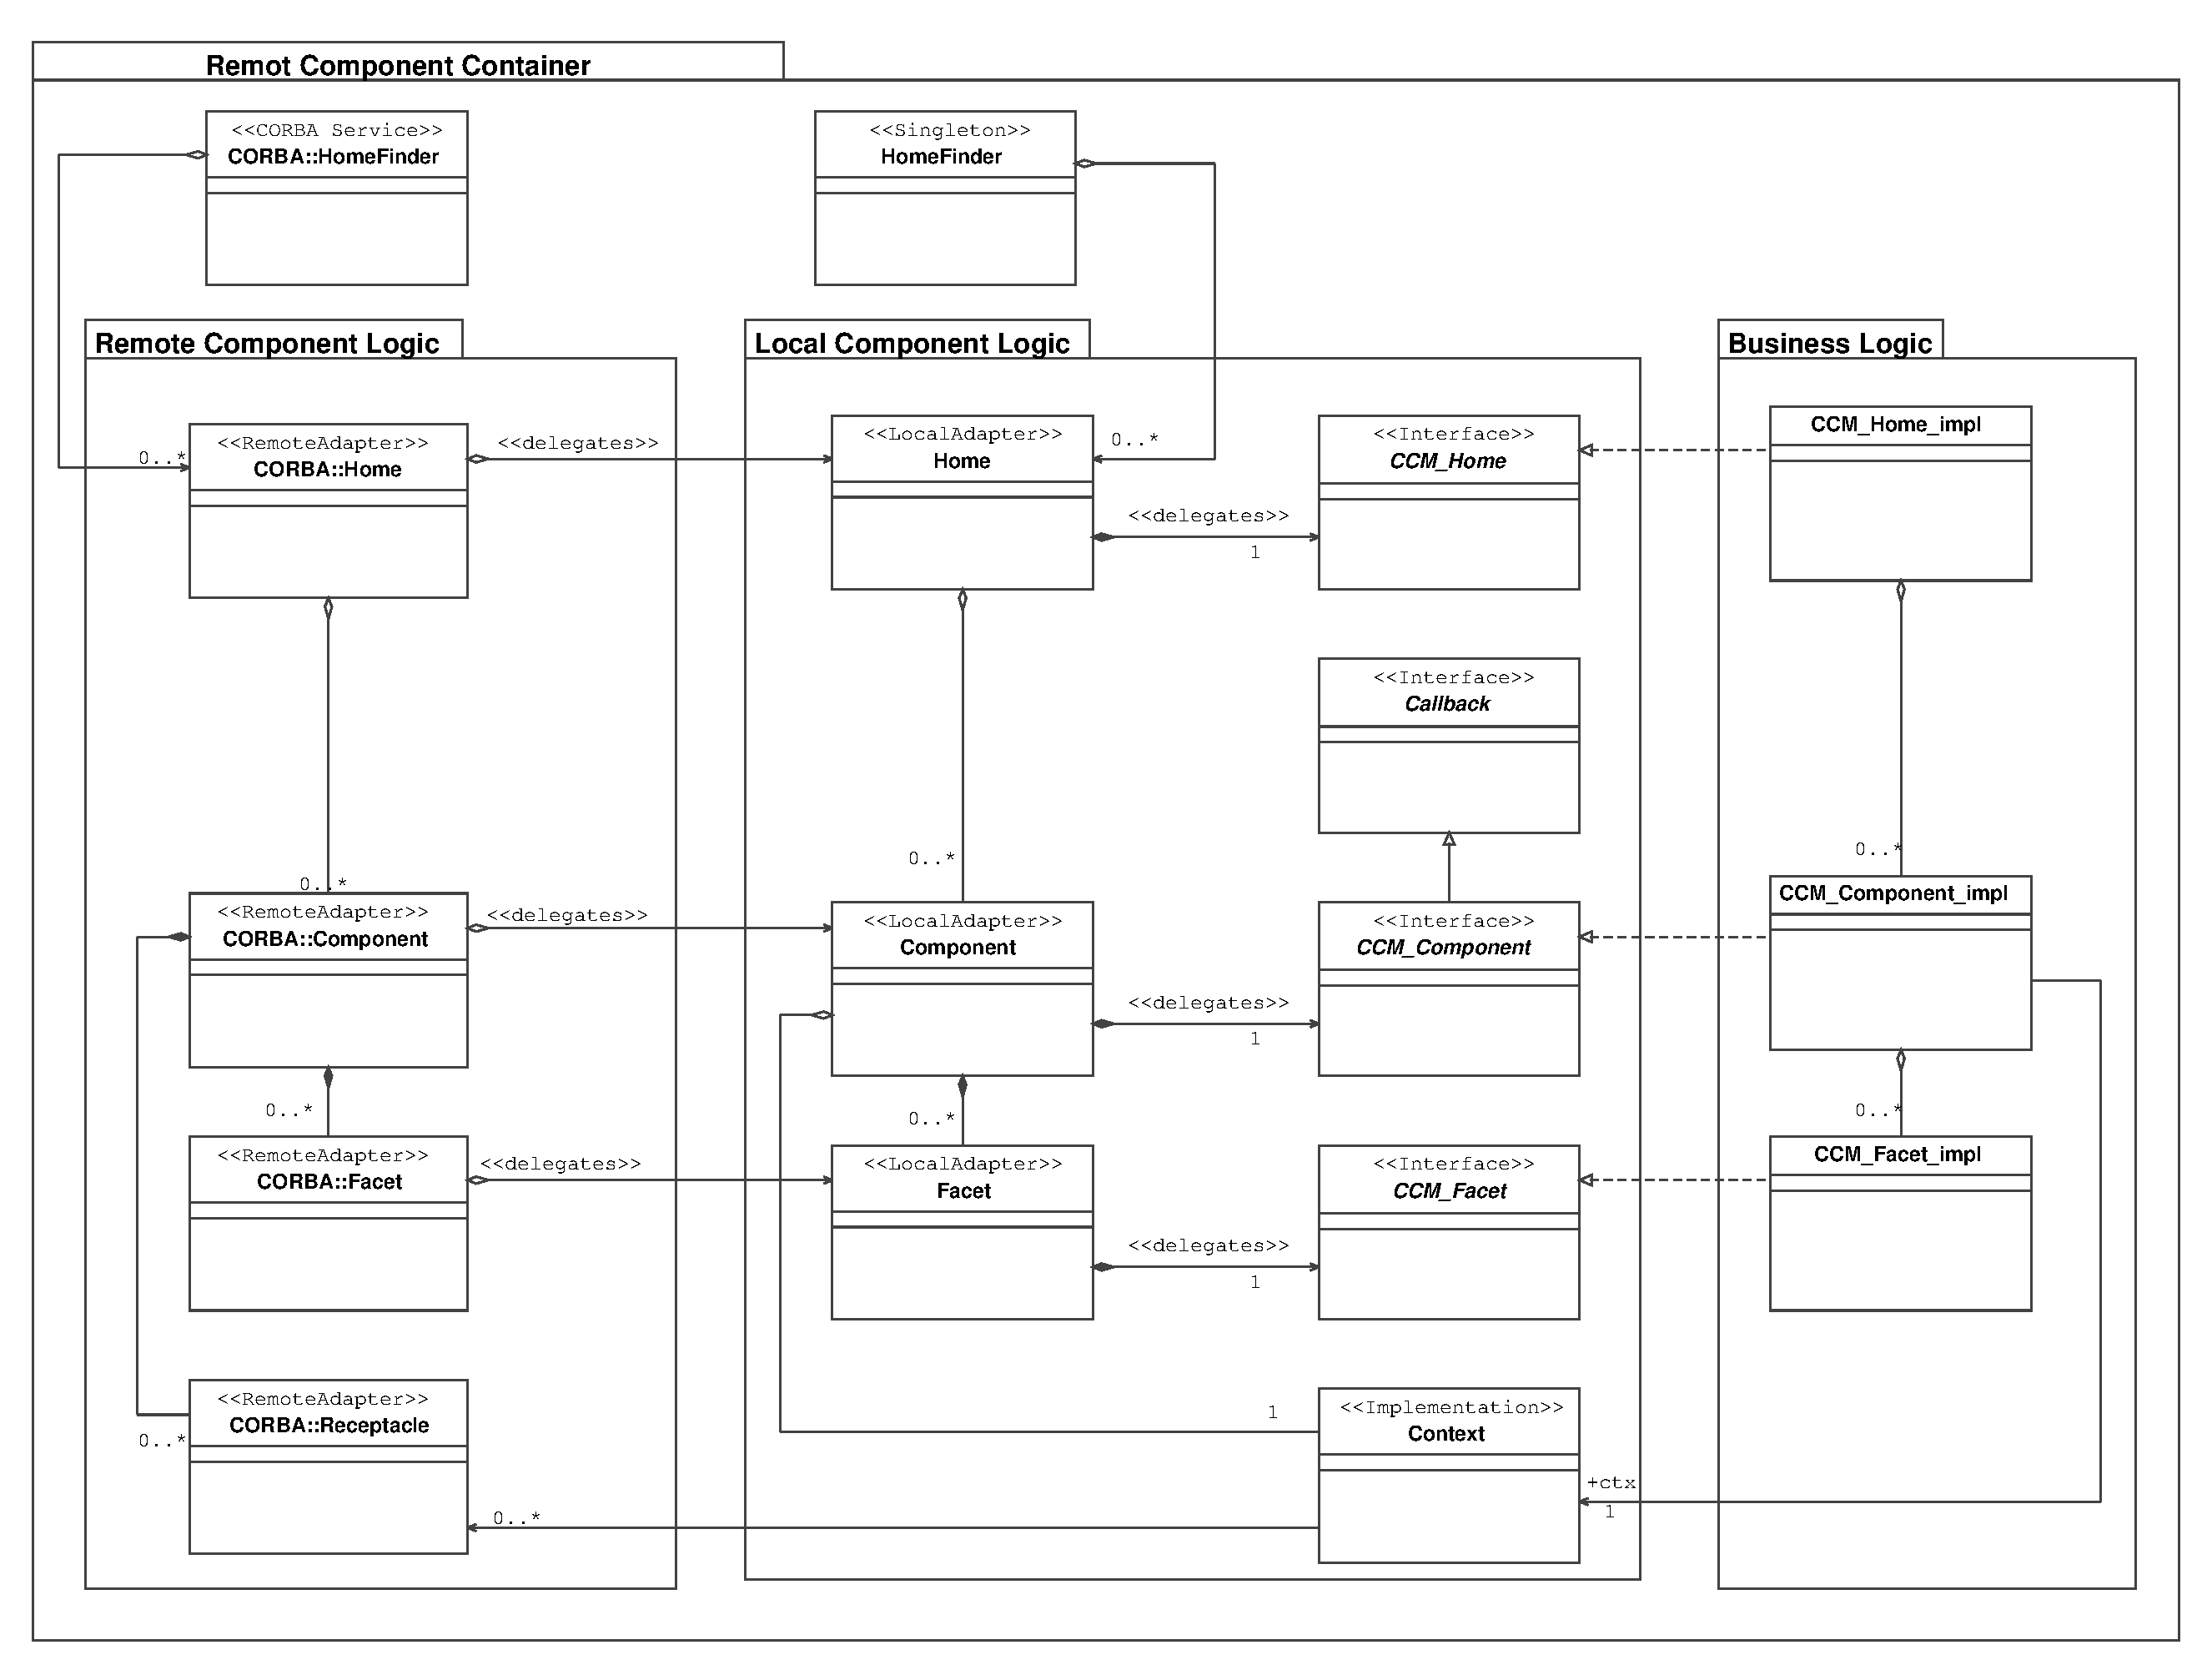
\includegraphics [width=15cm,angle=0] 
		     {uml/StructureOfRemoteComponents.eps}
    \caption{Simplified structure of a remote component implementation,
    showing the relationship between corresponding local and remote components.}
    \label{StructureOfRemoteComponents}            
    \end{center}
\end{figure}

\noindent
The remote structure is very similar to a local component's structure 
(Fig.~\ref{StructureOfLocalComponents}), thus, we can compare interactions
between a local and a remote component with interactions between business logic
and local component logic:

\begin{description}
\item [Calling component methods.]
A remote client calls methods on a remote adapter that delegates this
calls to a local component which uses a local adapter to delegate these calls
to business logic.
In each adapter, pre- and a post-invoke processing can take place 
(Fig.~\ref{RemoteComponentCall}).
\begin{figure}[htbp]
    \begin{center}
    \includegraphics [width=9cm,angle=0] 
		     {figures/RemoteComponentCall.eps}
    \caption{A remote call of a component's method is delegated twice
    allowing pre- and post-invoke processing.}
    \label{RemoteComponentCall}            
    \end{center}
\end{figure}

These two indirection layers allow non--functional extensions to 
components without changes in business logic. 
This separation of concerns is a cornerstone in component
based development.

\item [Invoking callback methods.]
Callback methods implemented by business logic can be
triggered either from local or remote component logic and their corresponding
container implementations to control a component's life cycle.

\item [Using context methods.]
Component business logic uses the {\tt Context} object to access container
functionality as well as component receptacles.
In the case of remote components, receptacles can be either local or remote
ports. Both kinds of receptacles can be accessed via local context
object methods. While local receptacles are connected directly to local facets,
remote receptacles are intercepted by a receptacle adapter.
\end{description}

\noindent
Based on LCAC, an existing LwCCM container implementation could be used to host 
local components, thus, we could combine an existing CORBA application server 
with the presented extensions in the context of local components. 


	% $Id$
%==============================================================================
\chapter{Login Example}
\label{chapter:LoginExample}
%==============================================================================

%******************************************************************************
\chapter{Introduction}
\label{chapter:introduction}
%******************************************************************************

The CCM Tools are a set of programs and libraries used to generate, package and
deploy CORBA components. The tools implement parts of the CCM specification
\cite{CCMSpecification} with some extensions to improve the usability and
performance of the component model. The {\it CCM Tools User's Guide\/} provides
instructions for using the CCM Tools. This document, the {\it CCM Tools
Developer's Manual\/}, is aimed at developers and provides details on the inner
workings of the CCM Tools.

\begin{figure}
\centering \includegraphics[width=14cm]{ToolsOverview}
\caption{Parts of the CCM Tools package.}
\label{fig:intro-ToolsOverview}
\end{figure}

To help the component developer, the CCM Tools provide the tools shown in
Figure~\ref{fig:intro-ToolsOverview}. These tools include the following parts:

\paragraph{CCM Metamodel Library}

The CCM specification defines a metamodel for the IDL3 syntax. This metamodel is
a set of classes that are capable of representing the syntactic elements in
IDL3. We implemented a metamodel library in Java that allows creation of, and
navigation through, CCM models. Using this library we can clearly separate the
parser and the code generators, using a CCM model as the communication between
the two parts. The parser creates a model object for every part of the source
code matching an IDL grammar rule, and the generator tools read the model to
generate code. Chapter~\cite{chapter:ccm-metamodel-library} describes the CCM
Tools' construction of the CCM metamodel library.

\paragraph{IDL3 Parser}

The IDL3 Parser reads an IDL3 file, checks the syntax of the IDL source code and
creates a CCM model, using the CCM metamodel library, in memory. This CCM model
is the starting point for all code generator tools.
Chapter~\cite{chapter:idl3-parser} describes the IDL3 parser in detail.

\paragraph{Mirror Component Generators}

After building a component it is a good idea to run a set of functional tests on
it. Such testing can provide helpful component specific debugging and prevent
large, difficult to locate, system bugs later in development.

To provide a test environment for every component, the CCM Tools can create a
mirror component (a facet becomes a receptacle and vice versa) described in a
mirror IDL3 file. We use the C++ component generators with the mirror IDL3 files
to generate the code for mirror components. Then we use a C++ mirror test
generator to create a basic test executable that connects each component with
its mirror and calls the functions available for each component.

\paragraph{IDL2 Generator}

To implement CORBA components, IDL3 source code needs to be reduced to IDL2,
which can be interpreted by classic IDL compilers. The transformation from IDL3
to IDL2 also adds some operations needed for navigation between components and
their ports (equivalent operations). The CCM Tools support this transformation
using an IDL2 generator tool that creates IDL2 code based on a CCM model.

\paragraph{Component Descriptor Generator}

To describe the component for the deployment and assembling processes, the OMG
defines a {\it CORBA Component Descriptor} (CCD) file. This is an XML file
containing a short description of a component and its ports. We map the CCM
model to an XML--DOM tree that can be written as an XML file. The CCD file is
also used by the code generators to get some additional information about the
components being generated (version, vendor, etc.).

\paragraph{Local C++ Component Generator}

The CCM Tools include a generator tool that creates the local component logic
from a given CCM model. The generated code contains C++ implementations of a
component that can run in the same address space (hence called a `local
component'). This implementation includes operations for providing, using,
connecting, and disconnecting components and their facets. These generated
operations are referred to as {\bf component logic}. After generating the
component logic, the component developer needs to write the {\bf business
logic}; that is, the functional implementation of the component so that it
becomes useful in a component based software system. See
Chapter~\cite{chapter:component-generator-tools} for more information about the
component generator library.

\paragraph{Remote C++ Component Generator}

Note that the local components can only be used in a common address space and
must be implemented in the same programming language. To overcome these
limitations, the CCM Tools have a remote component generator that produces C++
code to interface the local components with CORBA. The remote component logic is
thus a superset of the local component logic.

\paragraph{UML Parser}

Optionally, the description of the component's interfaces can be contained in a
UML diagram. We need a UML parser that reads the UML--XMI file, builds a UML
model (based on the UML metamodel defined by the OMG) and transposes the model
to a standard IDL3 file. The CCM Tools can use the NSUML UML metamodel library
from NovoSoft, but the OMG has not yet defined an UML profile for the CCM. Thus
a UML tool will likely be on the back burner for some time.

\paragraph{Component Packaging Tool}

After generating and writing the component logic and the component descriptor
file, we have to package these files into a zip file called, predictably, a
component package. The component packaging tool provides these functionalities
to the component developer.

\paragraph{Component Deployment Tool}

On the target host the component package must be unzipped and the component must
be deployed in the application server. The component deployment tool provides
these functionalities to the component deployer.

\section{Assembly tools}

After creating the component logic and writing the business logic, we can use
the component from a simple client program. A big advantage of the CORBA
component model is the ability to connect components together to form larger
structures called {\bf component assemblies}.

A component assembly is a set of components (with their component descriptors)
and a {\it Component Assembly Descriptor} (CAD). Based on the CAD we can
generate an assembly object that instantiates components and connects them
together to form a component assembly.

\begin{figure}
\includegraphics[width=14cm]{AssemblyTools}
\caption{CCM component assembly tools.}
\label{fig:intro-AssemblyTools}
\end{figure}

Figure~\ref{fig:intro-AssemblyTools} provides a diagram of the assembly tools in
the CCM Tools. These tools include:

\paragraph{Assembly Descriptor Generator}

The component descriptor files are the base for the higher--level assembly
descriptor, which describes the components of the assembly and their
connections. That means that all information of the assembly descriptor comes
from the component descriptors of the related components (and some additional
data from a GUI).

\paragraph{Assembly Object Generator}

At runtime a managing object is needed that can establish an assembly instance.
The assembly object creates the component instances and connects their
receptacles and facets. All information for generating an assembly object comes
from the assembly descriptor (or its DOM model in memory). Note that this object
must eventually be able to create local or local/remote assembly instances.

\paragraph{UML Parser}

As with components, there should be a way to define component assemblies in a
UML diagram. Therefore we need a UML parser that reads the UML--XMI file and
translates the data into the DOM model used by the assembly descriptor. The OMG
has not yet defined a mapping between UML and CCM assemblies.

\paragraph{Assembly Packaging Tool}

After generating the component assembly and its descriptor file we have to
package these files into a zip file called a component assembly package. The
assembly packaging tool provides these functionalities to the assembly
developer.

\paragraph{Assembly Deployment Tool}

On the target host the component assembly package must be unzipped and the
assembly must be deployed in the application server. The assembly deployment
tool provides these functionalities to the assembly deployer.

\section{Testing}

Another important issue is {\bf testing}. We have to test our applications on
different levels during development, as listed below:

\paragraph{Class Level Testing}

Every class of the business logic that will be part of a component has to be
tested.

\paragraph{Component Level Testing}

For every component we create a counter component that looks like a mirror to
the original component. This counter component has an receptacle for every facet
of the original component and vice versa. Connecting a component with its mirror
component with a simple test client allows component developers to quickly
isolate component level errors in the business code.

\paragraph{Assembly Level Testing}

After testing each component, we have to be sure that a set of connected
components, the component assembly, also works correctly.

Of course, there must be tool support for testing on these different levels of
development to make this job more efficient.


% $Id$
%==============================================================================
\section{Component Definition}
\label{section:ComponentDefinition}
%==============================================================================

We define components using the CCM Tools {\it Interface Definition Language}
(IDL), which is actually a subset of the CORBA IDL3 specification.
As shown in the following listing, a component definition can imply the
definition of a component home, one or more interfaces, operation parameters and
exceptions. 

\begin{footnotesize}
\begin{lstlisting}[language=IDL]
    module application
    {
        enum Group { GUEST, USER, ADMIN };

        struct PersonData
        {
            long id;
            string name;
            string password;
            Group group;
        };

        exception InvalidPersonData
        {
            string message;
        };

        interface Login
        {
            boolean isValidUser(in PersonData person)
              raises(InvalidPersonData);
        };

        component Server
        {
            provides Login login; 
        };

        home ServerHome manages Server { };
    };
\end{lstlisting}
\end{footnotesize}

\newpage

Here we can give only a short description of these IDL artefacts, you can find 
more information in chapter~\ref{chapter:InterfaceDefinitionLanguage} 
``Interface Definition Language`` of this manual.

\begin{itemize}
\item {\bf Modules} (e.g. {\tt application}).\\
Modules combine related IDL definitions into a logical group and prevent
pollution of the global namespace.  
   
\item {\bf User Defined Types} (e.g. {\tt Group}, {\tt PersonData}). \\
In addition to build--in types like {\tt long}, {\tt boolean}, {\tt string}, etc. a 
component designer can define its own types using, for example, {\tt enum} and {\tt struct} declarations.
Such user defined types can act as operation parameters as well as attribute types. 

\item {\bf Exceptions} (e.g. {\tt InvalidPersonData}). \\
To report an error condition, an operation can throw one or more exceptions. 
Befor we can declare an exception as part of an operation's raises section, we have to
define the exception which is pretty similar to defining a structure type.

\item {\bf Interfaces} (e.g. {\tt Login}). \\
An interface defines a named set of operations and attributes.
Each operation definition contains a result type, operation name, 
parameter list (which can be empty) and an optional exception list.
In IDL, each operation parameter includes a passing direction:
	\begin{itemize}
	\item {\tt in}: the parameter is passed from the caller to the 
					callee.
	\item {\tt out}: the parameter is passed from the callee back 
					to the caller.
	\item {\tt inout}: the parameter is passed from the caller to 
					the callee, modified and sent back to the caller.
	\end{itemize}


\item {\bf Components} (e.g. {\tt Server}): \\
A component uses interfaces to define input and output ports called facets 
and receptacles. 
While a facet's interface is implemented within its own component, a 
receptacle's interface uses implementations of connected facets of other 
components.


\item {\bf Component Homes} (e.g. {\tt ServerHome}): \\
To have an entry point for component instantiation, we define a component 
home. In the case of an empty home definition, a standard {\tt create()} 
operation will be generated from the CCM Tools.
\end{itemize}

From these few lines of IDL, we can generate a lot of structural code which 
implements all features of the CCM Tools component model, thus, you can 
focus on your business logic.

\newpage

% $Id$
%==============================================================================
\section{IDL Repository Directory}
\label{section:IdlRepositoryDirectory}
%==============================================================================

From the {\tt Login.idl} file, the CCM Tools generate an 
{\bf IDL Repository Directory}.
This {\tt idl3repo} directory contains all defined IDL artifacts in separated
files and in a uniform structure.
\begin{footnotesize}
\begin{verbatim}
	> ccmidl -idl3 -o ./idl3repo Login.idl
\end{verbatim}
\end{footnotesize}

After this step, you should see the following directory structure:
\begin{footnotesize}
\begin{verbatim}
        Login
        |-- Login.idl
        |-- idl3repo
        |   |-- component
        |   |   `-- application
        |   |       |-- Server.idl
        |   |       `-- ServerHome.idl
        |   `-- interface
        |       `-- application
        |           |-- Group.idl
        |           |-- InvalidPersonData.idl
        |           |-- Login.idl
        |           `-- PersonData.idl
\end{verbatim}
\end{footnotesize}

In this IDL repository, which is the starting point for all other CCM Tools
activities, there are two subdirectories:
\begin{itemize}
 	\item The {\tt interface} directory contains all IDL interface,
 	parameter, exception, etc. definitions.
 	  
  	\item The {\tt component} directory contains all component and
  	home definitions.
\end{itemize}

Each IDL artefact is stored in its own file within a directory that
conforms to the defined IDL module hierarchy.

\vspace{3mm}
For example, the interface {\tt Login} has been defined in the module 
{\tt application}, thus, this interface is stored in the directory 
{\tt interface/application} in a file named {\tt Login.idl} within the IDL 
repository.

\vspace{3mm}
From the developers point of view, it does not matter if the component
definitions are stored in a single or in multiple source files, the generated 
{\tt idl3repo} directory tree is the same in both cases.

 \newpage

% $Id$
%==============================================================================
\section{Use Case 1: Local C++ Components}
\label{section:LocalC++ComponentImplementation}
%==============================================================================

To introduce the first CCM Tools use case, we implement a local C++ component and a
collocated unit test. This use case is adequate for a developers who implements
large but modular C++ applications.

\vspace{3mm}
The implementation of local C++ components requires the following activities:
\begin{itemize}
	\item Model the component's structure in IDL 
			(see section~\ref{section:ComponentDefinition}). 
	\item Generate the local component logic.
	\item Implement the component's business logic.
	\item Implement a local component client.
\end{itemize}

It is an important point that modeling of IDL interfaces and components 
is completely independent of component implementations.
As you will see, we use IDL artifacts stored in the IDL repository directory
to generate both C++ and Java code.  
 
 
%------------------------------------------------------------------------------
\subsection{Generate the local component logic}
\label{subsection:GenerateComponentLogic}
%------------------------------------------------------------------------------

From the IDL repository directory the CCM Tools
generate a component skeleton which establishes the component's structure,
provides C++ interfaces to clients or other components, and uses the C++ runtime 
environment.
\begin{footnotesize}
\begin{verbatim}
> mkdir c++
> mkdir c++/server
> cd c++/server

> ccmtools c++local -I../../idl3repo/interface -I../../idl3repo/component \
                    -o ./src/interface                                    \
                    ../../idl3repo/interface/application/*.idl            

> ccmtools c++local -I../../idl3repo/interface -I../../idl3repo/component \
                    -a                                                    \
                    -o ./src/component/Server                             \
                    ../../idl3repo/component/application/Server*.idl
\end{verbatim}
\end{footnotesize}

After this code generation step, you can see the following directory structure:
\begin{footnotesize}
\begin{verbatim}
Login/c++/server
  `-- src
    |-- component
    |   `-- Server
    |       |-- CCM_application_ccm_local_component_Server
    |       |-- CCM_application_ccm_local_component_Server_share
    |       `-- application_ccm_local_component_Server_ServerHome_entry.h
    `-- interface
        |-- CCM_application_ccm_local
        `-- CCM_application_ccm_local_adapter
\end{verbatim}
\end{footnotesize}

Basically, all directories starting with '{\tt CCM\_}' contain component logic
which is completely generated (so there is no need to check--in these directories
into a CVS like system).
The component logic fills the gap between a component's interfaces and its
business logic implementation. 

\vspace{3mm}
Note that generated component logic can change between different CCM Tools
versions to improve component non functional behavior. Such changes do neither
affect component interfaces nor your business logic implementation which
realizes the functional behavior of components.   


%------------------------------------------------------------------------------
\subsection{Implement the component's business logic}
\label{subsection:ImplementC++BusinessLogic}
%------------------------------------------------------------------------------

Component business logic will be embedded in the generated component logic.
To make life easier, we used the {\tt -a} option during code generation.
This flag forces the code generator to generate application skeletons.

\vspace{3mm}
You can find these application skeletons {\tt *\_impl.* files} in the 
{\tt src/component/Server} subdirectory:
\begin{footnotesize}
\begin{verbatim}
Login/c++/server
  `-- src
    |-- component
    |   `-- Server
    |       |-- ServerHome_impl.cc
    |       |-- ServerHome_impl.h
    |       |-- Server_impl.cc
    |       |-- Server_impl.h
    |       |-- Server_login_impl.cc
    |       |-- Server_login_impl.h
\end{verbatim}
\end{footnotesize}

As a developer, you are responsible for these files because they represent the
component's business logic (you should check--in these files into a CVS like system).

\vspace{3mm}
There is a direct relationship between IDL and these business logic files:
\begin{itemize}
	\item {\tt ServerHome\_impl.*}\\
	For each component home, an implementation class is generated which provides an
	implementation of the default {\tt create()} operation.
	Additionally, the {\tt ServerHome\_impl.cc} file contains the implementation of
	the global: \\
    {\tt create\_application\_ccm\_local\_component\_Server\_ServerHome()} 
 	function which represents the business logic entry point used by the generated 
 	component logic. 

\item {\tt Server\_impl.*}\\
	For each component, an implementation class is generated which provides 
	default implementations of the component's callback operations.
	
\item {\tt Server\_login\_impl.*}\\
	For each facet, an implementation class is generated which provides empty
	business logic operation skeletons.
\end{itemize}

It is a good idea to generate these application skeletons only once - when starting 
component implementation. 
Small changes in IDL definitions can be appended pretty easy to these
implementation classes manually.

 \vspace{3mm}
Note that these implementation files are not overwritten by the CCM Tools.
The generator replaces only untouched source files, otherwise the
generated files are stored with a '{\tt .new}' suffix.

 \vspace{3mm}
To implement the Login example's business logic, you open the 
{\tt Server\_login\_impl.cc} file and implement the following code snippet:

\begin{footnotesize}
\begin{lstlisting}[language=C++]
bool
login_impl::isValidUser(
    const application::ccm::local::PersonData& person)
    throw(::ccm::local::Components::CCMException,
          application::ccm::local::InvalidPersonData )
{
    if(person.name.length() == 0)
        throw application::ccm::local::InvalidPersonData();

    if(person.id == 277 
       && person.name == "eteinik"
       && person.group == USER) 
    {
        return true;
    }
    else 
    {
        return false;
    }
}
\end{lstlisting}
\end{footnotesize}

Now, we can use Confix to build this component example. To tell Confix which
directory should be built, a {\tt Makefile.py} file must be created in each
source code directory.
Of course, you can delegate this work to the CCM Tools:
\begin{footnotesize}
\begin{verbatim}
> ccmconfix -makefiles -o ./src -pname "login" -pversion "1.0.0"
\end{verbatim}
\end{footnotesize} 

Finally, you start Confix to build all generated and manually implemented source
files:
\begin{footnotesize}
\begin{verbatim}
> confix.py --packageroot=`pwd`/src --bootstrap --configure --make 
\end{verbatim}
\end{footnotesize}

Now we are ready to test this local C++ component implementation.


%------------------------------------------------------------------------------
\subsection{Implement a local component client}
\label{subsection:ImplementLocalComponentClient}
%------------------------------------------------------------------------------

Instead of a real client with a complex GUI, we simply implement a unit test for
the component we have built in the last section.

\vspace{3mm}
We create a {\tt src/component/Server/test} directory and store the following
code in a file called {\tt \_check\_local\_component\_Server.cc}:
 
\begin{footnotesize} 
\begin{lstlisting}[language=C++]
#include <cassert>
#include <iostream>

#include <WX/Utils/debug.h>
#include <WX/Utils/smartptr.h>

#include <ccm/local/Components/CCM.h>
#include <ccm/local/HomeFinder.h>

#include <application/ccm/local/component/Server/Server_gen.h>
#include <application/ccm/local/component/Server/ServerHome_gen.h>

using namespace std;
using namespace WX::Utils;
using namespace ccm::local;
using namespace application::ccm::local;

int main(int argc, char *argv[])
{
  SmartPtr<component::Server::Server> server;
  SmartPtr<Login> login;
  Components::HomeFinder* homeFinder = HomeFinder::Instance();
  if(deploy_application_ccm_local_component_Server_ServerHome("ServerHome")) 
  {
      cerr << "ERROR: Can't deploy component homes!" << endl;
      return -1;
  }

  try 
  {
      SmartPtr<component::Server::ServerHome> serverHome(
        dynamic_cast<component::Server::ServerHome*>
          (homeFinder->find_home_by_name("ServerHome").ptr()));

      server = serverHome->create();
      login = server->provide_login();
      server->configuration_complete();

      // Implement your test cases here !!!
    
      server->remove();
  } 
  catch(Components::Exception& e ) 
  {
      cout << "ERROR: " << e.what() << endl;
      return -2;
  } 

  if(undeploy_application_ccm_local_component_Server_ServerHome("ServerHome")) 
  {
    cerr << "ERROR: Can't undeploy component home!" << endl;
    return -3;
  }
}
\end{lstlisting}
\end{footnotesize}

Each functional test case can be inserted into this unit test template shown above.
This code snipped is very similar for all simple component unit tests 
(see section~\ref{section:MirrorComponentConcept} for a more sophisticated test
setting).
It deploys the component home object, creates a component instance, uses 
the component's equivalent interface to get a facet, and completes the
configuration phase. 

\vspace{3mm}
After this setup process, we can execute our component test cases (we will
discuss the implementation of these test cases later).

\vspace{3mm}
Finally, we remove the component instance and undeploy the component home object.


\vspace{3mm}
Our first test case shows the usage of the {\tt Server} component and its 
{\tt login} facet. 
We fill the {\tt PersonData} structure with valid data and call the
{\tt isValidUser()} operation. Depending on the component's result we print out
a message to the console.

\begin{footnotesize}
\begin{lstlisting}[language=C++]
    try 
    {
        PersonData person;
        person.id = 277;
        person.name = "eteinik";
        person.password = "eteinik";
        person.group = USER;
	
        bool result = login->isValidUser(person);
        if(result) 
        {
            cout << "Welcome " << person.name << endl;
        }
        else 
        {
            cout << "Sorry, we don't know you !!!" << endl;
        }
    }
    catch(InvalidPersonData& e) 
    {
        cout << "Error: InvalidPersonData!!" << endl;
    }
\end{lstlisting}
\end{footnotesize}

The second test case shows the component's behavior for an invalid 
{\tt PersonData} structure. This test expects an {\tt InvalidPersonData}
exception to succeed.

\begin{footnotesize}
\begin{lstlisting}[language=C++]
    try 
    {
        PersonData person;
        person.id = 0;
        person.name = "";
        person.password = "";
        person.group = USER;

        login->isValidUser(person);
        assert(false);
    }
    catch(InvalidPersonData& e) 
    {
        cout << "OK, caught InvalidPersonData exception!" << endl;
    }
\end{lstlisting}
\end{footnotesize}

It is up to you to decide if you put both test cases into the same {\tt \_check\_*}
file or to implement each test case in its own file.

\vspace{3mm}
Note that each {\tt \_check\_*} file will end in a separate executable, thus,
for large applications you will need a lot of disk space.

\vspace{3mm}
To run these unit tests, we use Confix again:
\begin{footnotesize}
\begin{verbatim}
> touch src/component/Server/test/Makefile.py
> confix.py --packageroot=`pwd`/src --bootstrap --configure \
            --make --targets=check 
\end{verbatim}
\end{footnotesize}

At the end of this build process, you hopefully see an output like:
\begin{footnotesize}
\begin{verbatim}
Welcome eteinik
OK, caught InvalidPersonData exception!
PASS: login__check_local_component_Server
==================
All 1 tests passed
==================
\end{verbatim}
\end{footnotesize}

Of course, to implement a component for such a simple functionality is somewhat
academical, but this example shows how simple a component development cycle can
be by using CCM Tools. 

\newpage

% $Id$
%==============================================================================
\section{Use Case 2: Remote C++ Components}
\label{section:RemoteC++ComponentImplementation}
%==============================================================================

In the second CCM Tools use case, we implement a remote C++ component and a
remote unit test client based on CORBA middleware. 
This use case is adequate for a developers who implements large and distributed
C++ applications.

\vspace{3mm}
The implementation of remote C++ components requires the following activities:
\begin{itemize}
	\item Model a component's structure in IDL 
			(see section~\ref{section:ComponentDefinition}). 
	\item Implement a local C++ component (see section~\ref{section:LocalC++ComponentImplementation}).
	\item Generate remote component logic.
	\item Implement a remote component client.
\end{itemize}

For a given local C++ component implementation, you can generate a set of CORBA
adapters and converters which establish a remote component.
Thus, the step from local to remote C++ components is completely automated by
the CCM Tools.


%------------------------------------------------------------------------------
\subsection{Generate remote component logic}
\label{subsection:GenerateRemoteComponentLogic}
%------------------------------------------------------------------------------

Currently, we use CORBA middleware for inter--process communications, thus, local
interfaces must be adapted to CORBA objects and vice versa.

\vspace{3mm}
To implement CORBA interactions, we need CORBA stub and skeleton classes which
are generated by a particular IDL compiler. While components are modeled in
IDL3, usual IDL compilers assume IDL2 (no keywords like {\tt component} or 
{\tt home}).
For that reason, a separate CCM Tools generator transforms IDL3 to IDL2, as defined in
the CCM specification:
\begin{verbatim}
> ccmidl -idl2 -I../../idl3repo/interface -I../../idl3repo/component \
         -o src/component/Server/CCM_corba_stubs                     \  
         ../../idl3repo/interface/application/*.idl

> ccmidl -idl2 -I../../idl3repo/interface -I../../idl3repo/component \
         -o src/component/Server/CCM_corba_stubs                     \
         ../../idl3repo/component/application/Server*.idl
\end{verbatim}

All generated IDL2 files are stored in a directory called {\tt CCM\_corba\_stubs}:
\begin{verbatim}
    Login/c++/server
    |-- component
    |   `-- Server
    |       |-- CCM_corba_stubs
\end{verbatim}

We go into this {\tt CCM\_corba\_stubs} directory and call the IDL compiler for
every single file (fortunately, the CCM Tools provide a script that can do this
in a single call):
\begin{verbatim}
> cd src/component/Server/CCM_corba_stubs
> ccmtools-idl -mico -I${CCMTOOLS_HOME}/idl *.idl
> cd ../../../../
\end{verbatim}

The transformed IDL2 files include interfaces which are part of the
installed CCM Tools, thus, the IDL compiler needs the include path to {\tt CCMTOOLS\_HOME/idl} .

\vspace{3mm}
As a glue between the local C++ interfaces and the CORBA stubs and skeletons, we
generate some adapters and converters:
\begin{verbatim}
> ccmtools c++remote -I../../idl3repo/interface -I../../idl3repo/component \
                     -o src/component/Server/                              \
                     ../../idl3repo/interface/application/*.idl

> ccmtools c++remote -I../../idl3repo/interface -I../../idl3repo/component \
                     -o src/component/Server/                              \
                     ../../idl3repo/component/application/Server*.idl
\end{verbatim}

All new source files are stored in {\tt CCM\_*\_remote\_*} directories (we call
it remote component logic).
\begin{verbatim}
Login/c++/server
`-- src
    |-- component
    |   `-- Server
    |       |-- CCM_application_ccm_remote_component_Server
    |       |-- CCM_application_ccm_remote_corba_converter
    |       `-- CCM_corba_stubs
\end{verbatim}
Remember, there is no reason to check--in generated component logic into a CVS
like system because this code can be generated from the IDL repository directly.

\vspace{3mm}
That's it. We have extended our local C++ component from 
section~\ref{section:LocalC++ComponentImplementation} to a real remote component 
that can be accessed via CORBA
\footnote{
There is no technical reason to use only CORBA for remote communications.
Future versions of CCM Tools could provide other middleware (e.g. SOAP)
adapters too. } 
middleware.

%------------------------------------------------------------------------------
\subsection{Implement minimal CORBA server}
\label{subsection:ImplementMinimalCorbaAserver}
%------------------------------------------------------------------------------

Before implementing a remote client, we start the remote component as a
stand-alone CORBA server.
To keep things simple, we implement this CORBA server in a single 
{\tt \_check\_*.cc} file:
\begin{footnotesize}
\begin{lstlisting}[language=C++]
#include <string>
#include <WX/Utils/debug.h>
#include <CCM/CCMContainer.h>

#include <CORBA.h>
#include <coss/CosNaming.h>

#include <application/ccm/remote/component/Server/ServerHome_remote.h>
#include <application_Server.h>

using namespace std;
using namespace WX::Utils;

int main (int argc, char *argv[])
{
  char* argv_[] = { "", 
                    "-ORBInitRef", 
                    "NameService=corbaloc:iiop:1.2@localhost:5050/NameService"}; 
  int   argc_ = 3;
  CORBA::ORB_var orb = CORBA::ORB_init(argc_, argv_);

  // Register all value type factories with the ORB  
  CCM::register_all_factories(orb);

  // Deploy local and remote component homes	
  int error = 0;
  error += deploy_application_ccm_local_component_Server_ServerHome("ServerHome");
  error += deploy_application_ccm_remote_component_Server_ServerHome(orb, 
                                                                    "ServerHome");
  if(!error) 
  {
      cout << "ServerHome server is running..." << endl;
  }
  else 
  {
      cerr << "ERROR: Can't deploy components!" << endl;
      return -1;
  }
  orb->run();
}
\end{lstlisting}
\end{footnotesize}

We save this {\tt \_check\_application\_ccm\_remote\_component\_Server.cc} file
into the component's {\tt test} directory:
\begin{verbatim}
Login/c++/server
`-- src
    |-- component
    |   `-- Server
    |       `-- test
    |           `-- _check_application_ccm_remote_component_Server.cc
\end{verbatim}

A minimal CORBA server code initializes the ORB and deploys the local and
remote components. Remote component deployment implies the registration of the
component home object at the CORBA name service. 

\vspace{3mm}
Make sure that you run a CORBA name service on your box (e.g. {\tt orbd} which 
ist a Java tool):
\begin{verbatim}
> orbd -ORBInitialPort 5050
\end{verbatim}


Finally, we run Confix to build all source files and to start the unit test:
\begin{verbatim}
> ccmconfix -makefiles -o src -pname "login" -pversion "1.0.0"

> confix.py --packageroot=`pwd`/src --bootstrap --configure \
            --make --targets=check
\end{verbatim}

At the end of the build process, you should see the following line:
\begin{verbatim}
ServerHome server is running...
\end{verbatim}


%------------------------------------------------------------------------------
\subsection{Implement remote component client}
\label{subsection:ImplementRemoteComponentClient}
%------------------------------------------------------------------------------

We implement the remote component client as a simple unit test.
Because this client runs in a separate process (probably on a different machine), we
have to generate and build the CORBA stub and skeleton classes for the client 
again:

\begin{verbatim}
> ccmidl -idl2 -I../../idl3repo/interface -I../../idl3repo/component \
         -o src/component/Server/CCM_corba_stubs                     \  
         ../../idl3repo/interface/application/*.idl

> ccmidl -idl2 -I../../idl3repo/interface -I../../idl3repo/component \
         -o src/component/Server/CCM_corba_stubs                     \
         ../../idl3repo/component/application/Server*.idl
\end{verbatim}


In addition to the generated stubs and skeletons, we store the remote test
client in a file named {\tt \_check\_client.cc} within the following directory structure:
\begin{verbatim}
Login/c++/client
`-- src
    |-- component
    |   `-- Server
    |       `-- CCM_corba_stubs
    `-- test
        `-- _check_client.cc
\end{verbatim}

The remote client's implementation follows the local client's structure but uses
the IDL to C++ mapping specified by the OMG.

\begin{footnotesize}
\begin{lstlisting}[language=C++]
#include <string>
#include <WX/Utils/debug.h>
#include <CCM/CCMContainer.h>

#include <CORBA.h>
#include <coss/CosNaming.h>

#include <application_Server.h>
#include <application_ServerHome.h>

using namespace std;
using namespace WX::Utils;

int main (int argc, char *argv[])
{
    int   argc_   = 3;
    char* argv_[] = { "", 
                    "-ORBInitRef", 
                    "NameService=corbaloc:iiop:1.2@localhost:5050/NameService"};
 
    CORBA::ORB_var orb = CORBA::ORB_init(argc_, argv_);

    CORBA::Object_var obj = orb->resolve_initial_references("NameService");
    CosNaming::NamingContextExt_var nc = CosNaming::NamingContextExt::_narrow(obj);

    // Find ComponentHomes in the Naming-Service
    obj = nc->resolve_str("ServerHome");
    ::application::ServerHome_var home = ::application::ServerHome::_narrow(obj);

    // Create component instances
    ::application::Server_var server = home->create();
    ::application::Login_var login = server->provide_login();
    server->configuration_complete();

	// Run test cases
    try 
    {
      ::application::PersonData person;
      person.id = 277;
      person.name = CORBA::string_dup("eteinik");
      person.password = CORBA::string_dup("eteinik");   
      person.group =  ::application::USER;       
      
      CORBA::Boolean result = login->isValidUser(person);
      
      if(result) 
      {
          cout << "Welcome " << person.name << endl;
      }
      else 
      {
          cout << "We don't know you !!!" << endl;
      }
    }
    catch(::application::InvalidPersonData& e)
    {
      cout << "Error: InvalidPersonData" << endl;	
    }

    try 
    {
      ::application::PersonData person;
      person.id = 0;
      person.name = CORBA::string_dup(""); // Here we create an error!!!
      person.password = CORBA::string_dup("");   
      person.group =  ::application::USER;       
      
      login->isValidUser(person);
      assert(false); 
    }
    catch(::application::InvalidPersonData& e)
    {
      cout << "OK, caught InvalidPersonData exception!" << endl;	
    }

    // Destroy component instances
    server->remove();
}
\end{lstlisting}
\end{footnotesize}

Again, we use Confix to build and run the test client:
\begin{verbatim}
> ccmconfix -makefiles -o src -pname "login-remote-client" -pversion "1.0.0"

> confix.py --packageroot=`pwd`/src --bootstrap --configure \
            --make --targets=check
\end{verbatim}

When we see the following output on the console, we have successfully
implemented our first distributed component application:
\begin{verbatim}
Welcome eteinik
OK, caught InvalidPersonData exception!
PASS: login-remote-client__check_client
==================
All 1 tests passed
==================
\end{verbatim}

The important point is that we did not change the business logic implementation.
Instead, we reused the local component and generated a remote layer using the
CCM Tools.


\newpage
% $Id$
%==============================================================================
\section{Use Case 3: Local Java Components}
\label{section:LocalJavaComponentImplementation}
%==============================================================================

In this section, we implement a local Java component and a collocated test
client.
This CCM Tools use case is intended for developers who implement large and
modular Java applications. 

\vspace{3mm}
The implementation of local Java components requires the following activities:
\begin{itemize}
	\item Model the component's structure in IDL (see section~\ref{section:ComponentDefinition}). 
	\item Generate the local component logic.
	\item Implement the component business logic.
	\item Implement a collocated component client.
\end{itemize}

In the following sections, we use the IDL definitions stored in the IDL
repository directory as starting point for all Java code generations. 


%------------------------------------------------------------------------------
\subsection{Generate the local component logic}
\label{subsection:GenerateJavaComponentLogic}
%------------------------------------------------------------------------------
A local Java component logic includes a set of Java interfaces ({\tt -iface}
option) and a pure Java implementation ({\tt -local}) which
delegates client calls to the hosted business logic. 
Local Java component logic can be generated from the IDL repository using
the CCM Tools:
\begin{footnotesize}
\begin{verbatim}
> mkdir java
> mkdir java/server
> cd java/server
 
> ccmjava -iface -local                                         \
          -I../../idl3repo/interface -I../../idl3repo/component \ 
          -o ./src-gen                                          \
          ../../idl3repo/interface/application/*.idl

> ccmjava -iface -local                                         \
          -I../../idl3repo/interface -I../../idl3repo/component \
          -o ./src-gen                                          \
          ../../idl3repo/component/application/Server*.idl
\end{verbatim}
\end{footnotesize}

These code generation steps result in the following file structure:
\begin{footnotesize}
\begin{verbatim}
Login/java/server
`-- src-gen
    `-- application
        `-- ccm
            `-- local
\end{verbatim}
\end{footnotesize}

In contrast to C++ component logic, in Java we store all generated files in a
temporary {\tt src-gen} directory.


%------------------------------------------------------------------------------
\subsection{Implement the component business logic}
\label{subsection:ImplementBusinessLogicInJava}
%------------------------------------------------------------------------------
A set of generated interfaces act as the borderline between component-
and business logic. A business logic developer is free to realize the
implementation classes as long as the right interfaces will be implemented. 

\vspace{3mm}
As a CCM Tools feature, these implementation classes can be generated with
default implementations (mostly empty method skeletons).
These application class skeletons are generated in a separate directory called
{\tt src}: 
\begin{footnotesize}
\begin{verbatim}
> ccmjava -app                                                  \
          -I../../idl3repo/interface -I../../idl3repo/component \
          -o ./src                                              \
          ../../idl3repo/component/application/Server*.idl      
\end{verbatim}
\end{footnotesize}
Note the strict separation between generated component logic ({\tt src-gen})
and business logic ({\tt src}). 
As a developer, you are responsible for the {\tt src} directory tree - you
should use a CVS like code versioning system for this directory.
\begin{footnotesize}
\begin{verbatim}
Login/java/server
|-- src
|   `-- application
|       `-- ccm
|           `-- local
|               |-- ServerHomeFactory.java
|               |-- ServerHomeImpl.java
|               |-- ServerImpl.java
|               `-- ServerloginImpl.java
`-- src-gen
\end{verbatim}
\end{footnotesize}

\vspace{3mm}
There is a direct relationship between IDL definitions and generated business
logic skeleton classes:
\begin{itemize}
	\item {\tt ServerHomeFactory.java} \\
	For each component home, a factory class is generated which implements a {\tt create()}
	method that acts as entry point for business logic instantiation.
		  
	\item {\tt ServerHomeImpl.java}\\
	For each component home, an implementation class is generated which provides an
	implementation of the default {\tt create()} method.

\item {\tt ServerImpl.java}\\
	For each component, an implementation class is generated which provides 
	default implementations of the component's callback operations.
	
\item {\tt ServerloginImpl.*}\\
	For each facet, an implementation class is generated which provides
	skeletons for business logic implementations.
\end{itemize}

\vspace{3mm}
Note that these implementation files can not be overwritten by the CCM Tools.
Generators replaces only untouched implementation files, otherwise the 
re--generated files are stored with a '{\tt .new}' suffix.

 \vspace{3mm}
To implement the Login example's business logic, you can open the 
{\tt ServerloginImpl.java} file and implement the following code snippet:
\begin{footnotesize}
\begin{lstlisting}[language=Java]
public boolean isValidUser(PersonData person)
    throws CCMException, InvalidPersonData
{
    if(person.getName().length() == 0)
       throw new InvalidPersonData();
        
    if(person.getId() == 277
       && person.getName().equals("eteinik")
       && person.getGroup() == Group.USER)
    {
        return true;
    }
    else
    {
        return false;
    }
}    
\end{lstlisting}
\end{footnotesize}

Ant is used to build the Java component example. Here is an adequate
{\tt build.xml} file:
\begin{footnotesize}
\begin{verbatim}
<project name="LoginServer" default="compile">

  <property name="build" location="build" />
  <property name="src" location="src" />
  <property name="src-gen" location="src-gen" />

  <path id="compile.classpath">
      <pathelement path="${java.class.path}" />
  </path>

  <target name="init" description="" >
      <mkdir dir="${build}" />
  </target>
 
  <target name="compile" depends="init" description="" >
      <javac srcdir="${src-gen}:${src}" destdir="${build}" 
             debug="on" source="1.5" target="1.5">
          <classpath refid="compile.classpath" />  
      </javac>
  </target>

  <target name="clean" description="" >
      <delete dir="${build}" />
  </target>
</project>
\end{verbatim}
\end{footnotesize}

You can start the Ant build process with:
\begin{footnotesize}
\begin{verbatim}
> ant
\end{verbatim}
\end{footnotesize}

OK, you have implemented the firts Java component.


%------------------------------------------------------------------------------
\subsection{Implement a collocated component client}
\label{subsection:ImplementLocalComponentClient}
%------------------------------------------------------------------------------
To test the local component, a simple {\tt ClientLocal} class is implemented in 
the component's {\tt src} directory:
\begin{footnotesize}
\begin{verbatim}
Login/java/server
|-- src
|   |-- ClientLocal.java
|   `-- application
`-- src-gen
\end{verbatim}
\end{footnotesize}

The following listing shows a client's setup and tear down code. Before 
a component type can be used, we call the component's {\tt deploy()} method
which instantiates the component home object and register it to the local {\tt
HomeFinder} singleton.
On the other hand, before we terminate an application we call a
component's {\tt undeploy()} method to free the registered component home
object. 
	
\begin{footnotesize}
\begin{lstlisting}[language=Java]
import application.ccm.local.*;
import Components.ccm.local.HomeFinder;
import ccm.local.ServiceLocator;

public class ClientLocal
{
    public static void main(String[] args)
    {
        try
        {
            ServerHomeDeployment.deploy("ServerHome");
        }
        catch (Exception e)
        {
            e.printStackTrace();
        }

        // TODO: client's business logic implementation

        try
        {
            ServerHomeDeployment.undeploy("ServerHome");
        }
        catch (Exception e)
        {
            e.printStackTrace();
        }
    }
}
\end{lstlisting}
\end{footnotesize}

The next listing shows a client's business logic implementation. Note that all
interactions between client and component are based on generated interfaces.

\begin{footnotesize}
\begin{lstlisting}[language=Java]
try
{            
    HomeFinder homeFinder = ccm.local.HomeFinder.instance();
    ServerHome home = (ServerHome) homeFinder.find_home_by_name("ServerHome");
    Server server = home.create();
    server.configuration_complete();
    Login login = server.provide_login();
                        
    try
    {
        PersonData person = new PersonData(277, "eteinik", "eteinik", Group.USER);
        boolean result = login.isValidUser(person);

       if (result)
       {
           System.out.println("Welcome " + person.getName());
       }
       else
       {
           System.out.println("We don't know you...");
       }
    }
    catch (InvalidPersonData e)
    {
        System.err.println("Error: InvalidPersonData!");
    }

    try
    {
        PersonData person = new PersonData(0, "", "", Group.USER);
        login.isValidUser(person);
        assert(false);
    }
    catch (InvalidPersonData e)
    {
        System.err.println("OK, caught InvalidPersonData exception!");
    }

    server.remove();
}
catch (Exception e)
{
    e.printStackTrace();
}
\end{lstlisting}
\end{footnotesize}

To run this test, start the Ant build process and execute the local client
from the command line:
\begin{footnotesize}
\begin{verbatim}
> ant

> java -enableassertions                              \
       -cp $CCMTOOLS_HOME/lib/ccm-runtime.jar:./build \
       ClientLocal
\end{verbatim}
\end{footnotesize}

Now, you should see the following console output:
\begin{footnotesize}
\begin{verbatim}
Welcome eteinik
OK, caught InvalidPersonData exception!
\end{verbatim}
\end{footnotesize}

Well done! 

\newpage

% $Id$
%==============================================================================
\section{Use Case 4: Remote Java Components}
\label{section:RemoteJavaComponentImplementation}
%==============================================================================




\newpage
% $Id$
%==============================================================================
\section{Summary}
\label{section:LoginExampleSummary}
%==============================================================================

In this chapter, a lot of different CCM Tools use cases have been shown.
Each use case satisfies a particular architectural requirement, but
the main advantage of CCM Tools comes from a combination of these use cases. 

\begin{figure}[htbp]
    \begin{center}
        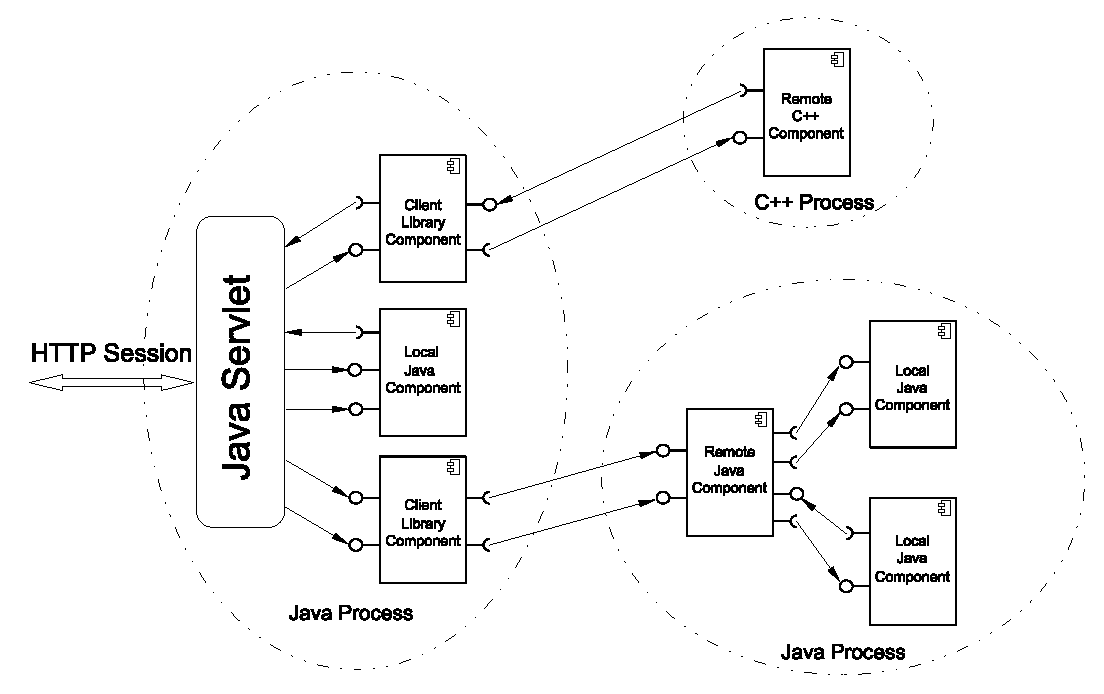
\includegraphics [width=14cm,angle=0] {figures/LoginSummary}
        \caption{Combining different CCM Tools use cases.}
        \label{figure:LoginSummery}
    \end{center}
\end{figure}

Fig.~\ref{figure:LoginSummery} shows a possible scenario where different use
cases are combined to realize a 	heterogeneous and distributed software system.
Based on CORBA middleware, we can interact between C++ and Java remote
components as well as between remote components and Java client library
components.

\vspace{3mm}
As component developers, we defined components in IDL and implement business
logic in generated implementation skeleton classes. 
Structural code needed to establish components which can be instantiated and 
connected via facts and receptacles, either local or remote, is completely generated by the
CCM Tools.






\newpage




	
	% $Id$
\begin{appendix}
%==============================================================================
	%$Id$

%==============================================================================
\chapter{CCM Tools Commands}
%==============================================================================

%------------------------------------------------------------------------------
\section{ccmconfix}
%------------------------------------------------------------------------------
\begin{description}
\item [NAME:] 
  {\tt ccmconfix} - Confix input files generator.

\item [SYNOPSIS:] 
  {\tt ccmconfix OPTIONS}

\item [DESCRIPTION:]
The {\tt ccmconfix} generator can be used to generate Confix input files.
Confix needs a {\tt Makefile.py} file in every source code directory (note that
Confix2 assumes {\tt Confix2.dir} and {\tt Confix.pkg} files instead of {\tt Makefile.py}).

\item [OPTIONS:]
  The {\tt ccmtconfix} generator handles the following options:
  \begin{itemize}
  \item {\tt -h,--help} \\
    Prints out a short description of the available command line parameters.

  \item {\tt -V, --version} \\
    Prints out the current version of installed CCM Tools.

  \item {\tt -o, --output <path> } \\
    Specifies the directory where the generation of Confix input files starts.
    The generator writes these files in the specified output directory as well
    as in every subdirectory (use the {\tt etc/ccmtools.properties} file to
    define a list of directories which will be ignored by the generator).

  \item {\tt -makefiles} \\
    Forces the generator to write {\tt Makefile.py} files as used by Confix 1.x.

  \item {\tt -confix2} \\
    Forces the generator to write {\tt Confix2.dir} and {\tt Confix.pkg} files as used by Confix 2.x.

  \item {\tt -pname, --packagename <name>} \\
  	Forces the generator to write {\tt PACKAGE\_NAME()} and  
	{\tt PACKAGE\_VERSION()} definitions in the top--level {\tt Makefile.py} (or the
	{\tt Confix2.pkg}) file.
  
  \item {\tt -pversion, --packageversion <version>} \\ 
    Specifies the used {\tt PACKAGE\_VERSION()} number. By default, a ``0.0.0'' string
    is used.
  \end{itemize}
    
\item [SEE ALSO:]
   {\tt Confix Manual}
\end{description}




%------------------------------------------------------------------------------
\section{ccmidl}
%------------------------------------------------------------------------------
\begin{description}
\item [NAME:] 
  {\tt ccmconfix} - Start script for IDL generators.

\item [SYNOPSIS:] 
  {\tt ccmidl OPTIONS FILES}

\item [DESCRIPTION:]
The {\tt ccmidl} script is used to run all kinds of IDL generator backends based
on a given set of IDL input files. 

\item [OPTIONS:]
  The {\tt ccmtconfix} generator handles the following options:
  \begin{itemize}
  \item {\tt -h, --help} \\
    Prints out a short description of the available command line parameters.

  \item {\tt -V, --version} \\
    Prints out the current version of installed CCM Tools.

  \item {\tt -I <path>} \\
    Specifies a path that will be used from a preprocessor to find 
    included IDL files.
  
  \item {\tt -o, --output <path> } \\
    Specifies the directory where the generated IDL files are stored to.

  \item {\tt -idl3 } \\
	Generates IDL3 source files for the IDL3 repository directory (for each IDL3
	artefact a separate source file will be generated).

  \item {\tt -idl3mirror } \\
  	Generates IDL3 source files for a mirror component.
  
  \item {\tt -idl2 } \\
  	Generates equivalent IDL2 source files which can be used as input for a
  	regular IDL compiler.
  \end{itemize}
    
  \item [FILES:]
  CCM Tools start scripts can handle single IDL files or a list of IDL
  files. The following examples show the usage of IDL files: 
  \begin{verbatim}
    ccmidl -idl3 -o idl3Repo *.idl
    ccmidl -idl3mirror -o idl3Repo Test.idl
    ccmidl -idl2 -o corba_stubs Test.idl Helper.idl 
  \end{verbatim}  
  
\item [SEE ALSO:]
\end{description}




%------------------------------------------------------------------------------
\section{ccmjava}
%------------------------------------------------------------------------------
\begin{description}
\item [NAME:] 
  {\tt ccmjava} - Start script for Java generators.

\item [SYNOPSIS:] 
  {\tt ccmidl OPTIONS FILES}

\item [DESCRIPTION:]
The {\tt ccmidl} script is used to run all kinds of Java generator backends based
on a given set of IDL input files. 

\item [OPTIONS:]
  The {\tt ccmtjava} generator handles the following options:
  \begin{itemize}
  \item {\tt -h, --help} \\
    Print out a short description of the available command line parameters.

  \item {\tt -V, --version} \\
    Print out the current version of installed CCM Tools.

  \item {\tt -I <path>} \\
    Specify a path that will be used from a preprocessor to find 
    included IDL files.
  
  \item {\tt -o, --output <path> } \\
    Specify the directory where the generated IDL files are stored to.

  \item {\tt -iface } \\
	Generate local Java interface definitions from the given IDL files. 

  \item {\tt -local } \\
	Generate local Java component logic implementations for the given IDL files.  

  \item {\tt -app } \\
	Generate buisness logic skeletons for the given IDL files.

  \item {\tt -remote } \\
  	Generate remote Java component logic implementations for the given IDL files.
  
  \item {\tt -clientlib } \\
	Generate local Java component proxies which are used to access remote
	components via local Java interfaces.
  \end{itemize}
    
  \item [FILES:]
  CCM Tools start scripts can handle single IDL files or a list of IDL
  files. The following examples show the usage of IDL files: 
  \begin{verbatim}
    ccmjava -iface -o  *.idl
    ccmjava -iface -local -app -o src-gen Test.idl TestHome.idl
  \end{verbatim}  
  
\item [SEE ALSO:]
\end{description}





\newpage
%------------------------------------------------------------------------------
\section{ccmtools}
%------------------------------------------------------------------------------

\begin{description}

\item [NAME:] 
  {\tt ccmtools} - Frontend to start available CCM Tools generators.

\item [SYNOPSIS:] 
  {\tt ccmtools TYPE [OPTIONS] FILES}

\item [DESCRIPTION:]
The {\tt ccmtools} script is used to run a particular component 
generator backend based on a set of IDL files. 
Depending on {\tt TYPE} and {\tt OPTIONS} a particular code generator is 
selected to create the desired output.

\item [TYPE:]
  Currently, the following generator types are supported:
  \begin{itemize}
  \item {\tt c++local}\\
    Generates local C++ component logic.
    
  \item {\tt c++local-test} \\
    Generates a test client for a pair of local C++ component and
    mirror component.
    
  \item {\tt c++dbc} \\
    Generates a set of Design by Contract adapters for a local
    C++ component.

  \item {\tt c++remote} \\ 
    Generates a set of remote C++ adapters that establish a standard
    compliant CORBA component where a local C++ component can be embedded.

  \item {\tt c++remote-test}\\
    Generates a test client for a pair of remote component and mirror component.
    
  \item {\tt idl3 }\\  (!!! deprecated !!!) \\
    Generates IDL3 source files.

  \item {\tt idl3mirror }\\ (!!! deprecated !!!)\\
    Generates IDL3 source files for a mirror component.
    
  \item {\tt idl2}\\ (!!! deprecated !!!) \\
    Generates equivalent IDL2 source files.
  \end{itemize}
  
\item [OPTIONS:]
  In addition to the generator types, the {\tt ccmtools} script handles
  the following options:
  \begin{itemize}
  \item {\tt -a, --application} \\
    Forces the local C++ generator to create business logic
    implementation skeletons ({\tt *\_impl.*} files).

  \item {\tt -h, --help} \\
    Prints out a short description of the available command line parameters.

  \item {\tt -Ipath} \\
    Specifies a path that will be handled from a preprocessor to find 
    included IDL files.

  \item {\tt -o DIR, --output=DIR} \\
    Specifies the directory where the generated code will be written. 

  \item {\tt -V, --version} \\
    Prints out the current version of installed CCM Tools.
  \end{itemize}
  
\item [FILES:]
  This {\tt ccmtools} script can handle single IDL files or a list of IDL
  files. The following examples show the usage of IDL files: 
  \begin{verbatim}
    ccmtools c++local -a -o test Test.idl Helper.idl 
    ccmtools c++local-test -o test *.idl
    ccmtools idl3mirror -o test/idl3mirror Test.idl
  \end{verbatim}
\item [SEE ALSO:] {\tt ccmidl}
\end{description}




%------------------------------------------------------------------------------
\section{ccmtools-idl}
%------------------------------------------------------------------------------

\begin{description}

\item [NAME:] 
  {\tt ccmtools-idl} - Run an IDL compiler to generate CORBA stub and skeletons.

\item [SYNOPSIS:] 
  {\tt ccmtools-idl OPTION FILES}

\item [DESCRIPTION:]
  The {\tt ccmtools-idl} script is a IDL compiler wrapper for Mico ORB and Java ORB,
  and hides the different call notations. This script also allows to process more than
  one IDL file at the same time. 
  Note that this script assumes that both IDL compilers are installed correctly.

\item [OPTION:]
  The {\tt ccmtools-idl} script supports of the following options:
  \begin{itemize}
  \item {\tt -h, --help} \\
    Prints out a short description of the available command line parameters.

  \item {\tt -Ipath} \\
    Specifies a path that will be handled from a preprocessor to find 
    included IDL files.
   
  \item {\tt --mico} \\
    Forces the use of Mico's IDL compiler.
    Thus, the generated stub and skeletons are implemented in C++.

  \item {\tt --java} \\
    Forces the use of Java's build in IDL compiler.
    Thus, the generated stub and skeletons are implemented in Java.
    Note that Java's IDL compiler only supports CORBA 2.x but no CORBA 3.0 extensions
    like {\tt component}, {\tt home}, etc.

  \item {\tt -V, --version} \\
    Prints out the current version of installed CCM Tools.
  \end{itemize}
  
\item [FILES:]
  This {\tt ccmtools-idl} script can handle single IDL files or a list of IDL
  files. The following examples show the usage of IDL files: 
  \begin{verbatim}
    ccmtools-idl --mico CarRental.idl
    ccmtools-idl --java CarRental.idl Customer.idl
    ccmtools-idl --mico *.idl
  \end{verbatim}

\item [SEE ALSO:]
  {\tt Mico manual, Java IDL documentation}
\end{description}



%------------------------------------------------------------------------------
\section{uml2idl}
%------------------------------------------------------------------------------

\begin{description}

\item [NAME:] 
  {\tt uml2idl} - Convert an UML XMI file into an IDL and an OCL file. 

\item [SYNOPSIS:] 
  {\tt uml2idl XMI-FILE PREFIX}

\item [DESCRIPTION:]
  The {\tt uml2idl} script runs a Java program that converts a UML diagram stored
  in an XMI 1.1 file into corresponding IDL and OCL files.
  The IDL file is created in respect to the {\it UML Profile for CCM}, while the
  OCL file collects all OCL expressions defined in the UML diagram.

\item [XMI-FILE:]
  That's the name of the input XMI 1.1 file which holds the UML class diagram
  (e.g. when using MagicDraw 9.0, the file name looks like {\tt Name.xml.zip}).

\item [PREFIX:]
  The generated IDL and OCL files are named {\tt PREFIX.idl} and {\tt PREFIX.ocl}.

\item [SEE ALSO:]
  {\tt UML Profile for CORBA, UML Profile for CCM}
  
\end{description}

	% $Id$
%==============================================================================
\chapter{CCM Tools Installation}
%==============================================================================


%------------------------------------------------------------------------------
\section{Prerequisites}
%------------------------------------------------------------------------------

To install the CCM Tools, the following programs must be available:
\begin{description}
\item [Java SDK $\ge$ 1.5.x] ({\tt http://java.sun.com/j2se})
\item [Apache Ant $\ge$ 1.6.x] ({\tt http://ant.apache.org})
\item [Python $\ge$ 2.4.x] ({\tt http://python.org})
\item [cpp $\ge$ 3.3.x] ({\tt http://www.gnu.org})
\end{description}

To build the generated C++ components, we also need:
\begin{description}
\item [Confix $\ge$ 1.5.x] ({\tt http://confix.sourceforge.net})
\item [gcc $\ge$ 3.3.x] ({\tt http://www.gnu.org})
\item [mico $\ge$ 2.3.11] ({\tt http://www.mico.org/})
\end{description}


%------------------------------------------------------------------------------
\section{How to get it}
%------------------------------------------------------------------------------

The project is hosted at Sourceforge ({\tt http://ccmtools.sf.net}). See the web
site for releases and announcements.

You can also subscribe to the {\tt ccmtools-announce} mailing list for CCM Tools
release announcements. The {\tt ccmtools-users} mailing list provides a forum
for discussion about using the CCM Tools.


%------------------------------------------------------------------------------
\section{Binary distribution}
%------------------------------------------------------------------------------

Installing the CCM Tools from a binary package is quite simple:
\begin{small}
\begin{verbatim}
$ tar xvzf ccmtools-x.y.z-bin.tar.gz 
\end{verbatim}
\end{small}

\noindent
This package comes with the following structure:
\begin{small}
\begin{verbatim}
ccmtools-x.y.z
|-- bin
|-- lib
`-- templates
    |-- CppLocalTemplates
    |-- CppLocalTestTemplates
    |-- CppRemoteTemplates
    |-- CppRemoteTestTemplates
    |-- IDL2Templates
    |-- IDL3MirrorTemplates
    `-- IDL3Templates
\end{verbatim}
\end{small}

\noindent
Finally, you can set your environment variables:

\begin{small}
\begin{verbatim}
 $ export CCMTOOLS_HOME=<CCM_INSTALL_PATH>
 $ export PATH=$CCMTOOLS_HOME/bin:$PATH	    

 # Additionally, the following settings are needed for using remote
 # components based on the Mico ORB
 $ export CCM_NAME_SERVICE=corbaloc:iiop:1.2@localhost:5050/NameService
 $ export CCM_COMPONENT_REPOSITORY=${CCMTOOLS_HOME} 
 $ export CCM_INSTALL=<MY_INSTALL_PATH>
\end{verbatim}
\end{small}

\noindent
Note that you also need a C++ runtime environment to compile and run the
generated components.
These C++ runtime packages must be installed from source.


\newpage
%------------------------------------------------------------------------------
\section{Source distribution}
%------------------------------------------------------------------------------


%------------------------------------------------------------------------------
\subsection{CCM Tools package:}
%------------------------------------------------------------------------------
Installing the CCM Tools from source requires the following steps:

\begin{small}
\begin{verbatim} 
 $ tar xvzf ccmtools-x.y.z.tar.gz
\end{verbatim}
\end{small}

\noindent
Alternatively, you can check out an up-to-date version from CVS:
\begin{small}
\begin{verbatim}
 $ cvs -d :pserver:anonymous@ccmtools.cvs.sf.net:/cvsroot/ccmtools login
 Password: <press enter>
 $ cvs -d :pserver:anonymous@ccmtools.cvs.sf.net:/cvsroot/ccmtools co ccmtools
\end{verbatim}
\end{small}

\noindent
To build the CCM Tools we use Ant: 
\begin{small}
\begin{verbatim}
 $ cd ccmtools
 $ ant install -Dprefix=<CCM_INSTALL_PATH>
\end{verbatim}
\end{small}

\noindent
Don't forget to set your environment variables properly
(as described in the 'Binary distribution' section). 


%------------------------------------------------------------------------------
\subsection{Java runtime package:}
%------------------------------------------------------------------------------
To access remote CCM components from Java clients, we have to install
a Java client's runtime environment called {\tt java-environment}:

\begin{small}
\begin{verbatim}
 $ tar xvzf java-environment-x.y.z.tar.gz
\end{verbatim}
\end{small}

Alternatively, you can check out an up-to-date version from CVS:
\begin{small}
\begin{verbatim}
 $ cvs -d :pserver:anonymous@ccmtools.cvs.sf.net:/cvsroot/ccmtools \
       co java-environment
\end{verbatim}
\end{small}

To build and install the java-environment we use Ant:
\begin{small}
\begin{verbatim}
 $ cd java-environment
 $ ant install -Dprefix=<CCM_INSTALL_PATH>
\end{verbatim}
\end{small}

\noindent
To used this runtime library from a Java client, 
don't forget to set the {\tt CLASSPATH} variable:
\begin{small}
\begin{verbatim}
 $ export CLASSPATH=<CCM_INSTALL_PATH>/lib/Components.java:$CLASSPATH
\end{verbatim}
\end{small}



%------------------------------------------------------------------------------
\subsection{C++ runtime packages:}
%------------------------------------------------------------------------------
As shown in Fig.~\ref{ccmtools-structure}, to compile and run generated CCM
components, we need a C++ runtime environment.

\noindent
To build and install C++ environment packages as well as generated C++ components, 
we use {\tt Confix}. 
{\tt Confix} is a build tool that is based on {\tt automake} and 
{\tt autoconf} - visit the {\tt confix.sf.net} page to read the
exhaustive manual. 

\noindent
It's a good idea to create a CCM Tools profile in Confix' configuration file
({\tt .confix}), as described in the Confix manual.
\begin{small}
\begin{verbatim}
ccm_tools_profile = {
    'PREFIX': '<MY_INSTALL_PATH>',        # use your own path!
    'BUILDROOT': '<MY_BUILD_PATH>',       # use your own path!
    'ADVANCED': 'true',
    'USE_LIBTOOL': 'true',
    'CONFIX': {
    },
    'CONFIGURE': {
       'ENV': {
          'CC': 'gcc',                     # use your own path!
          'CXX': 'g++',                    # use your own path!    
          'CFLAGS': "-g -O0 -Wall",
          'CXXFLAGS': "-g -O0 -Wall",
          },
       'ARGS': [
        '--with-mico=<MICO_INSTALL_PATH>/lib/mico-setup.sh'
	# use your own mico install path!
       ]
    },
}

PROFILES = {
    'ccmtools': ccm_tools_profile,
    'default' : ccm_tools_profile
}
\end{verbatim}
\end{small}

\noindent
It's important that you substitute your own paths in the {\tt .confix} file.\\
We can configure the {\tt ccm\_tools\_profile} as default profile, thus we 
don't need to use the {\tt --profile=ccmtools} confix option.
Additionally, we advise to set the {\tt ADVANCED} flag to {\tt true} instead of
using the {\tt --advanced} command--line option. 


\noindent
To install the CCM Tools runtime packages, the following steps are needed: 

\begin{small}
\begin{verbatim}
 $ tar xvjf wx-toolsbox-x.y.z.tar.bz2
 $ cd wx-toolsbox-x.y.z
 $ confix.py --bootstrap --configure --make --targets="install"

 $ tar xvjf wx-utils-x.y.z.tar.bz2
 $ cd wx-utils-x.y.z
 $ confix.py --bootstrap --configure --make --targets="install"

 $ tar xvzf cpp-environment-A.B.X.tar.gz
 $ cd cpp-environment
 $ confix.py --packageroot=`pwd`/ccm --bootstrap --configure \
             --make --targets="install"
\end{verbatim}
\end{small}

Note that you can alternatively check out an up-to-date version of the
{\tt cpp-environment} package from CVS:
\begin{small}
\begin{verbatim}
 $ cvs -d :pserver:anonymous@ccmtools.cvs.sf.net:/cvsroot/ccmtools \
       co cpp-environment
\end{verbatim}
\end{small}

Perfect, all tools and libraries have been installed and are ready to work!






	%==============================================================================
\chapter{A CCM Overview}
%==============================================================================
\begin{flushright}
{\it }
\end{flushright}

%==============================================================================
\section{Introduction}
%==============================================================================
The {\it Object Management Group} (OMG) has been standardizing an open
middleware specification to support distributed applications. The OMG specified
an sophisticated component model based on the {\it Common Object Request Broker
Architecture} (CORBA) called {\it CORBA Component Model} (CCM)
\cite{CCMSpecification}.



%==============================================================================
\section{Component model}
%==============================================================================

The CCM defines a component architecture and a container framework in which the
component life cycle takes place.
\begin{figure}[htbp]
    \begin{center}
        \includegraphics [width=6cm,angle=0] {Component}
        \caption{CCM component}
        \label{component}
    \end{center}
\end{figure}

A {\it CCM Component} (Fig.~\ref{component}) provides a variety of surface
features that support ways to connect components together to form assemblies:
\begin{description}
\item [Home] 
The component home is an interface that defines factory and finder methods to
create or find component instances managed by the home. Each home supports at
least one {\tt create} method.

\item [Equivalent interface]
Every IDL3 interface (containing the keywords {\tt component}, {\tt home}, etc.)
will be transformed into a classic IDL interface that can be processed by a
regular IDL compiler -- the equivalent interface. This IDL3 to IDL mapping adds
some interfaces and equivalent operations to the user written interfaces. As
described by the CCM specification, every IDL3 construct defines its own IDL3 to
IDL mapping.

\item [Supported interface]
A home or component definition can support zero or more interfaces that results
in inheritance of supported interfaces in the corresponding equivalent
interfaces.

\item [Attribute]
Component or a component home can have attributes that are named values exposed
through accessor and mutator operations. Attributes are primarily intended to be
used for component configuration.

\item [Facet]
A component's facet is a named interface that provides access to specific
component methods. A component may have zero ore more facets. The component's
equivalent interface inherits the {\tt Components::Navigation} interface that
defines generic operations for facet access.

\item [Receptacle]
A component's receptacle is an abstraction that is concretely manifested on a
component as a set of operations for establishing and managing connections. A
component may have zero ore more receptacles. The component's equivalent
interface inherits the {\tt Components::Receptacles} interface that defines
generic operations for receptacle management.

\item [Event source]
An event source embodies the potential for the component to generate events of a
specified type and provides mechanisms for associating consumers with sources.
There are two categories of event sources, {\it emitters} and {\it publishers}.
An emitter can be connected to at most one proxy provider by the container. A
publisher can be connected through the channel to an arbitrary number of
consumers that are subscribed to the publisher event source.

\item [Event sink]
An event sink embodies the potential for the component to receive events of a
specified type.
\end{description}

The component model is also defined in a MOF compliant metamodel, the {\it
Interface Repository Metamodel}, that expresses the extensions to classic IDL
defined by the CCM.


%==============================================================================
\section{Component container}
%==============================================================================

Components run in a {\it CCM Container} (Fig.~\ref{container}) that provides the
runtime environment for CORBA components. Containers are built on the {\it
Object Request Broker} (ORB), the {\it Portable Object Adapter} (POA) and CORBA
services.

\begin{figure}[htbp]
    \begin{center}
        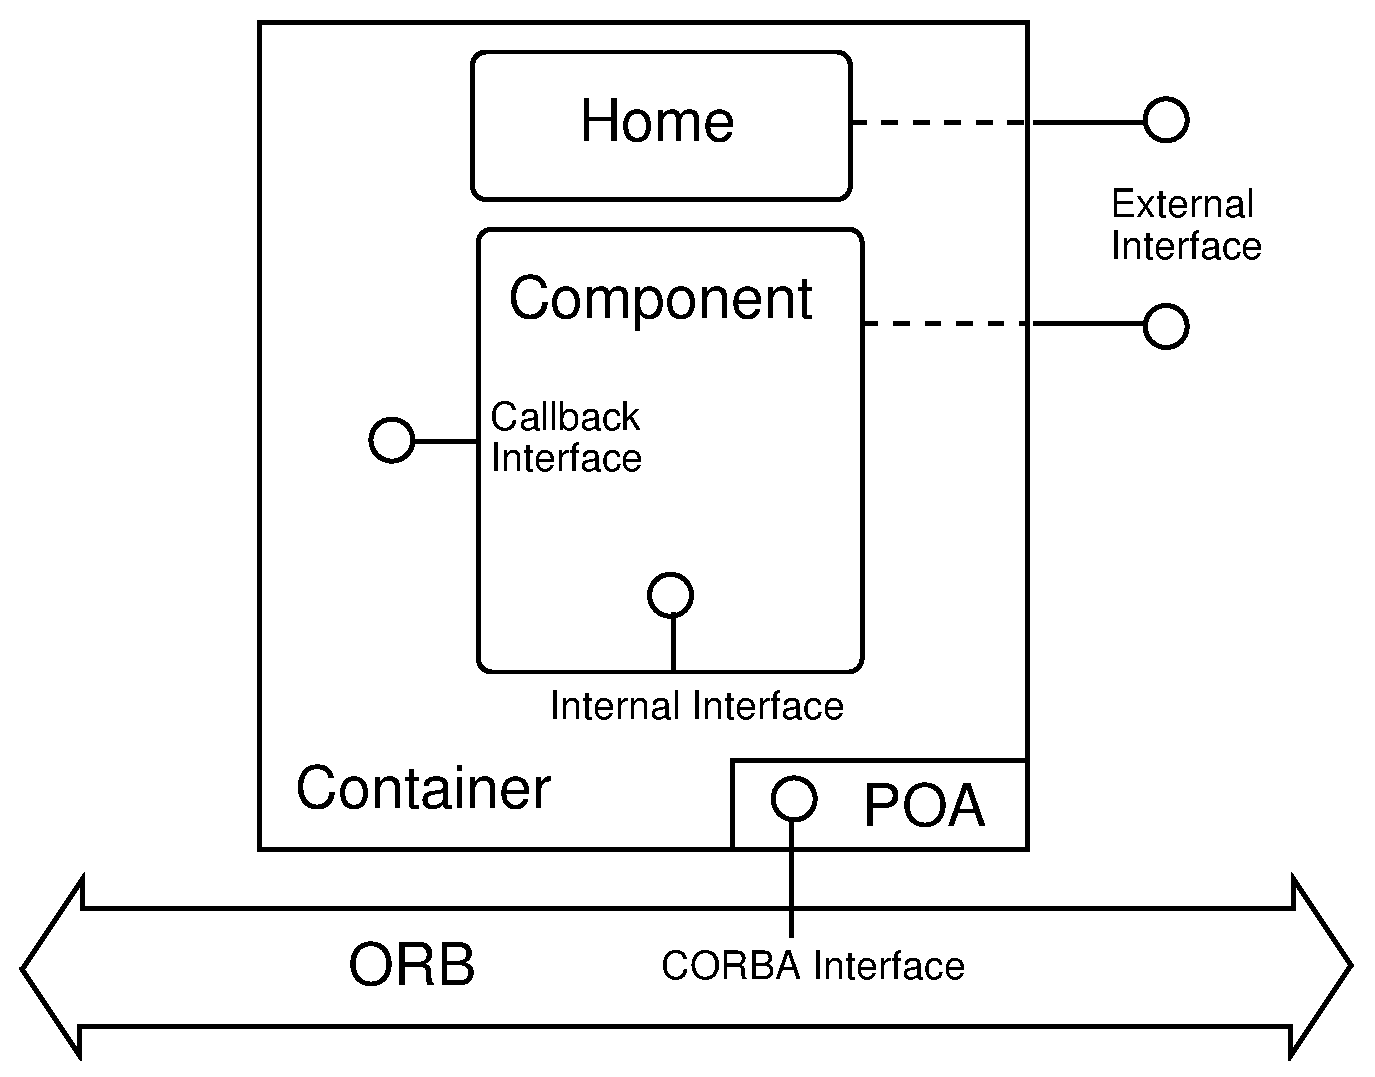
\includegraphics [width=6cm,angle=0] {Container}
        \caption{CCM container}
        \label{container}
    \end{center}
\end{figure}

As shown in Fig.~\ref{container}, the container programming model is made of the
following interfaces that are used by the client, the container and the
components:
\begin{description}
\item [Internal interfaces]
These local interfaces are used by the component developer and provided by the
container to assist in the implementation of the component's behavior.

\item [External interfaces] The external interfaces define the external view of
a component. They are used by the client and implemented by the component
developer.

\item [Callback interfaces]
These local interfaces are used by the container and implemented by the
component, either in generated code or directly, in order for the component to
be deployed in the container.
\end{description}

The CCM specification defined component categories whose behavior is specified
by the two container API types. Additionally there is a component category that
describe the empty container.
\begin{description}
\item [Service component]
The service component has behavior, no state and no identity. The lifespan of a
service component is equivalent to the lifetime of a single operation request.

\item [Session component]
The session component has behavior, transient state and a identity that is not
persistent. Note that the session component is equivalent to the stateful
session bean found in EJB.

\item [Process component]
The process component has behavior, persistent state which is not visible to the
client, and a persistent identity.

\item [Entity component]
The entity component has behavior, persistent state which is visible to the
client, and a identity which is visible to the clients through a primary key
declaration.

\end{description}



%==============================================================================
\section{Component assembly}
%==============================================================================

Connecting components by their ports leads to component {\it Assemblies} as
shown in Fig.~\ref{assemblygraph}.

\begin{figure}[htbp]
    \begin{center}
        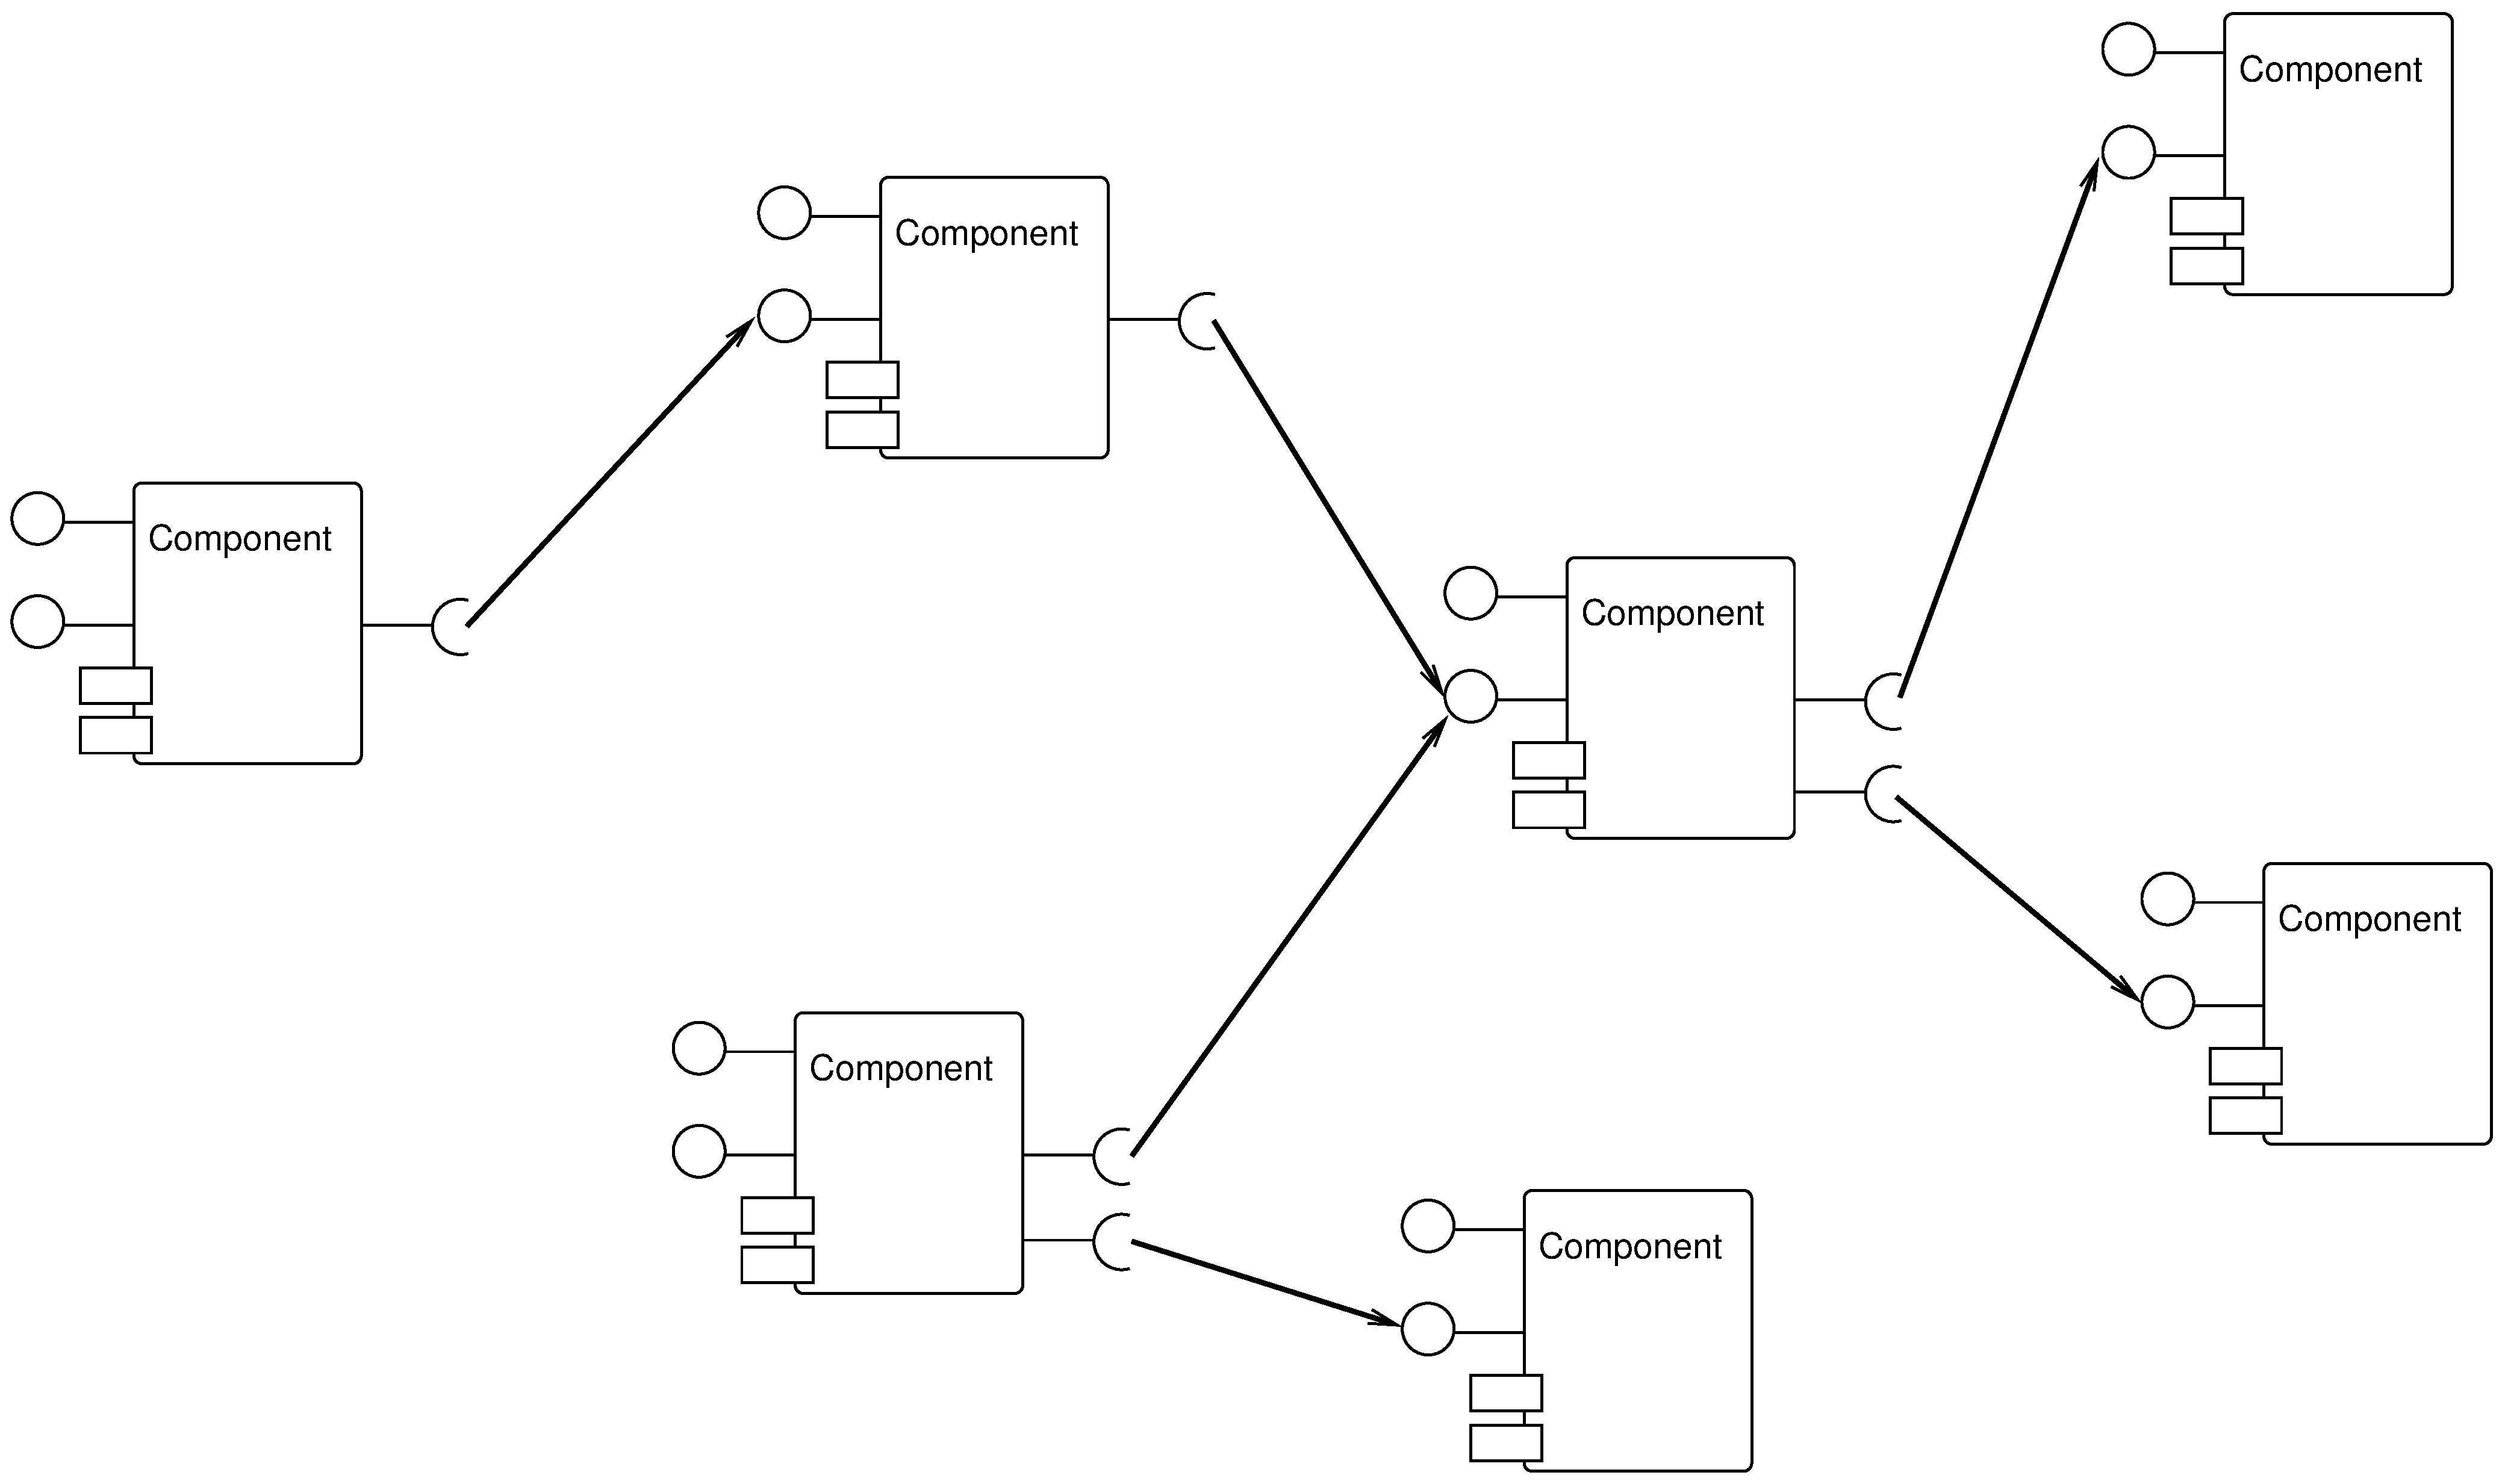
\includegraphics [width=6cm,angle=0] {Assembly}
        \caption{Component assembly}
        \label{assemblygraph}
    \end{center}
\end{figure}

The CCM specification defines an {\tt Components::Assembly} interface that
represents an assembly instantion. It is used to build up and tear down
component assemblies. Building the assembly up means creating all of the
components and establish connections between them as specified in the assembly
descriptor. Tearing the assembly down means removing all connections and
destroying the components.


%==============================================================================
\section{Descriptor files}
%==============================================================================

The CCM specification defines a bunch of XML descriptor files that are used to
describe software packages, components, properties and assemblies.
\begin{description}
\item [Software package descriptor (*.csd)]
The software package descriptor consists of general information about the
software followed by one or more sections describing implementations of
software.

\item [CORBA component descriptor (*.ccd)]
The component descriptor specifies component characteristics that a design tool
my use to display information about a component (e.g. supported interfaces,
inherited components, used and provided ports, etc.).

\item [Component assembly descriptor (*.cad)]
The assembly descriptor consists of elements describing the components used in
the assembly, connection information and partitioning information.

\item [Property file descriptor (*.cpf)]
The property file is used at deployment time to configure a home or a component
instance. A configurator uses the property file to determine how to set
component and home property attributes.
\end{description}


%==============================================================================
\section{Client programming model}
%==============================================================================

The client interacts with a CORBA component through two forms of external
interfaces, a home interface and one or more application interfaces. Two forms
of clients are supported by the CCM specification:
\begin{description}
\item [Component--aware client] 
This client knows that it is making requests against a component. The client can
use component mechanisms like navigation between component and facets etc.
Component--aware clients locates their interfaces using the {\tt
Components::HomeFinder} or a naming service.

A reference that supports the {\tt HomeFinder} interface may be obtained from
the ORB by invoking {\tt CORBA::ORB::resolve\_initial\_references()} with the
parameter value {\tt ``ComponentHomeFinder''}.

\item [Component--unaware client]
This client does not know that there is a CORBA component, the client requests
to ordinary CORBA objects and object factories.
\end{description}




	% $Id$
%==============================================================================
\section{Light Weight CORBA Component Model}
%==============================================================================

Many of today's embedded CORBA applications are unable to use the available 
enterprise CCM due to design constraints.
These constraints include small code size in embedded environments and 
limited processing overhead for performance conservative applications.

\vspace{3mm}
\noindent
To overcome this problem, LwCCM
was submitted to the OMG \cite{LwCCM-Specification}.
The purpose of this profile is to specify a lightweight version of the CCM.
The principal aim of LwCCM is to have a component model sufficient to compose
applications with CORBA components without all optional features that are
not part of the ``core'' capabilities of CCM.
%This profile exposes what mandatory features should be contained in a 
%minimum implementation of the CCM. 
The choices made in the profile follow rules established to suit embedded
environments:
\begin{itemize}
\item {\bf Redundancy.}
If several ways of requesting a service exist, only one is retained.

\item {\bf Interoperability and Compatibility with full CCM.}
During deployment, a leightweight component should be deployable by a full
CCM deployment application. Connections between a leightweight component
and a full CCM component must be possible.
Implementations of leightweight components should be source compatible
with the full CCM.

\item {\bf Persistence.}
The LwCCM does not need to manage any kind of persistence as described in the
CCM specification. 

\item {\bf Transactions.}
Transactions are not a feature commonly used in embedded systems thus they
are not included in the LwCCM profile.

\item {\bf Security.}
Security will not be treated in the LwCCM profile.

\item {\bf Introspection.}
Not all introspection operations are retained in this profile because they
are not essential to perform the deployment of components.

\item {\bf EJB Integration.}
There is no integration of {\it Enterprise JavaBeans} defined in LwCCM
because EJB are not required for embedded targeted environments.

\item {\bf Deployment and Configuration.}
Instead of the {\it Packaging and Deployment} chapter of CCM, LwCCM
is based on the OMG {\it Deployment and Configuration} specification 
\cite{DeploymentAndConfiguration}.
This includes also the definitions of component and assembly descriptor
files and their XML DTDs.

\item {\bf CCM Implementation Framework.}
The whole {\it Component Implementation Definition Language} (CIDL) chapter 
as well as the {\it CCM Implementation Framework} (CIF) chapter are excluded 
from the LwCCM profile.

The CIDL is redundent with IDL definitions because all functional descriptions
of the component (facets, reseptacles, events and attributes) is done with the 
IDL files.
The way to assign a component category (service or session) to a component
can be done via an XML description file that will be used with the IDL files to
generate container code and skeletons.
\end{itemize}

\noindent
This profile tries to be as compliant as possible to the OMG 
{\bf Minimum CORBA} and {\bf Lightweight Services} specifications 
\cite{Minimum_CORBA, LightweightServices}.



%==============================================================================
\end{appendix}


%=References===================================================================
\bibliographystyle{plain}
\bibliography{bibtex/cbse,bibtex/doc,bibtex/wx,bibtex/pattern,bibtex/se,bibtex/mda}
%==============================================================================
\end{document}
